\documentclass[11pt,letterpaper]{article}
\usepackage{authblk}
% \usepackage[utf8]{inputenc}
\usepackage{amsthm}
\usepackage{amsfonts}
\usepackage{amsmath}
\usepackage{amssymb}
\let\amssquare\square
\usepackage{mathtools}
% \usepackage{stmaryrd}
% \usepackage{tensor}
\usepackage[mathscr]{eucal}
\usepackage{url}
% \usepackage{marvosym}
\usepackage[left=2cm,right=2cm,top=2cm,bottom=2cm]{geometry}
%\usepackage{geometry}
\usepackage{minted}
\usepackage{cite}

\usepackage{tikz-cd}
\usetikzlibrary{positioning}
\usetikzlibrary{fit}
\usetikzlibrary{cd}
\usetikzlibrary{arrows}
\usetikzlibrary{calc}
\usetikzlibrary{decorations.markings}
\tikzset{ed/.style={auto,inner sep=2pt,font=\scriptsize}} %edges
\tikzset{>=stealth'}
\tikzset{vert/.style={draw,circle, minimum size=6mm, inner sep=0pt, fill=white}}
\tikzset{vertbig/.style={draw,circle, minimum size=8mm, inner sep=0pt, fill=white}}
\tikzset{->-/.style={decoration={
      markings,
      mark=at position #1 with {\arrow{>}}},postaction={decorate}}}

\usepackage[hidelinks]{hyperref} % Should be imported LAST

\theoremstyle{plain}
\newtheorem{theorem}{Theorem}[subsection]
% \newtheorem{axiom}[theorem]{Axiom}
\newtheorem*{theoremstar}{Theorem}
% \newtheorem{fact}[theorem]{Fact}
\newtheorem{proposition}[theorem]{Proposition}
\newtheorem{lemma}[theorem]{Lemma}
\newtheorem{corollary}[theorem]{Corollary}

\theoremstyle{definition}
\newtheorem{definition}[theorem]{Definition}
% \newtheorem{convention}[theorem]{Convention}
% \newtheorem{construction}[theorem]{Construction}
\newtheorem{example}[theorem]{Example}
% \newtheorem{examples}[theorem]{Examples}
% \newtheorem{notation}[theorem]{Notation}
\newtheorem{remark}[theorem]{Remark}
% \newtheorem{idea}[theorem]{Idea}
% \newtheorem{question}[theorem]{Question}

\newcommand{\C}{\mathscr{C}}
\newcommand{\homC}{\underline{\C}}
\newcommand{\D}{\mathscr{D}}
\newcommand{\E}{\mathscr{E}}
\newcommand{\M}{\mathscr{M}}
\newcommand{\N}{\mathscr{N}}
\newcommand{\T}{\mathscr{T}}

\newcommand{\bN}{\mathbb{N}}
\newcommand{\bZ}{\mathbb{Z}}

\newcommand{\lenslib}{\texttt{lens}}

\newcommand{\Pastro}{\Phi}
% \newcommand{\Pastro}{\mathrm{Pastro}}
\newcommand{\Double}{\mathcal{D}}

% Categories
\newcommand{\Set}{\mathbf{Set}}
\newcommand{\Cat}{\mathbf{Cat}}
%\newcommand{\Hask}{\mathbf{Hask}}
\newcommand{\Prof}{\mathbf{Prof}}
\newcommand{\Core}{\mathbf{Core}}
\newcommand{\MonCat}{\mathbf{MonCat}}
\newcommand{\LaxMonCat}{\mathbf{LaxMonCat}}
\newcommand{\SymmMonCat}{\mathbf{SymmMonCat}}
\newcommand{\Tele}{\mathbf{Tele}}
\newcommand{\Tamb}{\mathbf{Tamb}}

\newcommand{\Endo}{\mathbf{Endo}}
\newcommand{\Strong}{\mathbf{Strong}}
\newcommand{\Point}{\mathbf{Point}}
\newcommand{\CoPoint}{\mathbf{CoPoint}}
\newcommand{\App}{\mathbf{App}}
\newcommand{\Traversable}{\mathbf{Traversable}}
\newcommand{\IdxTraversable}{\mathbf{IdxTraversable}}

\newcommand{\Act}{\mathbf{Act}}
\newcommand{\Optic}{\mathbf{Optic}}
\newcommand{\Lawful}{\mathbf{Lawful}}
%\newcommand{\SemiOptic}{\mathbf{SemiOptic}}
\newcommand{\Lens}{\mathbf{Lens}}
\newcommand{\Prism}{\mathbf{Prism}}
\newcommand{\Setter}{\mathbf{Setter}}
\newcommand{\Traversal}{\mathbf{Traversal}}
\newcommand{\Getter}{\mathbf{Getter}}
\newcommand{\Review}{\mathbf{Review}}
\newcommand{\Fold}{\mathbf{Fold}}

\newcommand{\switched}{\mathbin{\tilde{\otimes}}}

\newcommand{\conc}{\mathbb{C}}
\newcommand{\conctwice}{\mathbb{C}^2}

\newcommand{\id}{\mathrm{id}}
\newcommand{\op}{\mathrm{op}}
\newcommand{\const}{\mathrm{const}}
\DeclareMathOperator{\ob}{ob}
\DeclareMathOperator{\copr}{copr}
\newcommand{\inl}{\mathrm{inl}}
\newcommand{\inr}{\mathrm{inr}}
\DeclareMathOperator{\im}{im}

\newcommand{\rep}[2]{{\ensuremath \left\langle #1 \mid #2 \right\rangle}}
\newcommand{\repthree}[3]{{\ensuremath \langle #1 \mid #2 \mid #3 \rangle}}
\newcommand{\repfour}[4]{{\ensuremath \langle #1 \mid #2 \mid #3 \mid #4 \rangle}}

\newcommand{\fget}{\textsc{Get}}
\newcommand{\fput}{\textsc{Put}}
\newcommand{\fmodify}{\textsc{Modify}}
\newcommand{\freview}{\textsc{Review}}
\newcommand{\fcreate}{\textsc{Create}}
\newcommand{\fmatching}{\textsc{Matching}}
\newcommand{\funzip}{\textsc{Unzip}}
\newcommand{\fover}{\textsc{Over}}

\newcommand{\mget}{\textsc{MGet}}
\newcommand{\mput}{\textsc{MPut}}
\newcommand{\munzip}{\textsc{Munzip}}

\newcommand{\inside}{\mathsf{inside}}
\newcommand{\outside}{\mathsf{outside}}
\newcommand{\once}{\mathsf{once}}
\newcommand{\twice}{\mathsf{twice}}

% Credit: Sam Buss
%\newbox\gnBoxA
%\newdimen\gnCornerHgt
%\setbox\gnBoxA=\hbox{$\ulcorner$}
%\global\gnCornerHgt=\ht\gnBoxA
%\newdimen\gnArgHgt
%\def\nameof #1{%
%    \setbox\gnBoxA=\hbox{$#1$}%
%    \gnArgHgt=\ht\gnBoxA%
%    \ifnum     \gnArgHgt<\gnCornerHgt \gnArgHgt=0pt%
%    \else \advance \gnArgHgt by -\gnCornerHgt%
%    \fi \raise\gnArgHgt\hbox{$\ulcorner$} \box\gnBoxA %
%    \raise\gnArgHgt\hbox{$\urcorner$}}

% Special arrows
%\newcommand{\isoto}{\xrightarrow{\cong}}
\newcommand{\hto}{\ensuremath{\,\mathaccent\shortmid\rightarrow\,}}

\makeatletter
\providecommand{\leftsquigarrow}{%
  \mathrel{\mathpalette\reflect@squig\relax}%
}
\newcommand{\reflect@squig}[2]{%
  \reflectbox{$\m@th#1\rightsquigarrow$}%
}
\makeatother

% Draft helpers
\newcommand{\todo}[1]{\textcolor{red}{\small #1}}

\newif\ifhideproofs
% \hideproofstrue %uncomment to hide proofs
\ifhideproofs
\usepackage{environ}
\NewEnviron{hide}{}
\let\proof\hide
\let\endproof\endhide
\fi

\title{Categories of Optics}
\author{Mitchell Riley}
\affil{Wesleyan University \\ \texttt{mvriley@wesleyan.edu}}
\begin{document}
\maketitle

\section{Introduction}

In its most concrete form, a \emph{lens} from $S$ to $A$ is a pair of maps $\fget : S \to A$ and $\fput : S \times A \to S$. From a software engineering standpoint, such a lens allows us to ``zoom in'' on $S$ to focus on a small part $A$, manipulate $A$ in some way, then ``zoom out'' and have our changes reflected in $S$. 

We consider a lens well-behaved if it obeys the following laws: 
\begin{itemize}
\item ``$\fput\fget$'': $\fget \; \fput = \pi_2$ as maps $S \times A \to A$, so that any update to $A$ should be represented faithfully in $S$;
\item ``$\fget\fput$'': $\fput [\id_S, \fget] = \id_S$ as maps $S \to S$, so that if $A$ is not changed then $S$ should not change; and,
\item ``$\fput\fput$'': $\fput (\fput \times A) = \fput \, \pi_{1, 3}$ as maps $S \times A \times A \to S$, so any update to $A$ completely overwrites previous updates.
\end{itemize}
We will call such lenses \emph{lawful}. (The names of the laws make more sense when the equations are written with composition in diagrammatic order!)

%\todo{reference a whole bunch of bx and database stuff}

Lenses were discovered to be just one of a hierarchy of data accessors, including prisms, setters, traversals, and more, collectively called \emph{optics}. Each optic variant has a concrete description as a certain collection of maps, with attendant laws under which we consider them well-behaved. We begin in Section~\ref{sec:optics} by defining the \emph{category of optics} in a sufficiently general way to encompass almost all the optic variants in use in the wild. Section~\ref{sec:lawful-optics} defines the equivalent of the lens laws for a generic category of optics. Then in Section~\ref{sec:examples} we see that these generic definitions specialise correctly to all the basic varieties of optic, including giving the correct laws.

The widely used Haskell \lenslib{} library contains implementations of all these optic variants: see \cite{LensLibrary}. There, optics are written in a form known as the \emph{profunctor encoding}, which at first glance is completely different to that given in Section~\ref{sec:optics}. As this note was being written, Bartosz Milewski~\cite{ProfunctorOpticsPost} independently described the relationship between some forms of optic and their profunctor encoding. In Section~\ref{sec:profunctor-optics} we extend this to more of the optic hierarchy and translate the laws into the profunctor setting.

\todo{Indexed optics?}

More recently, concrete lenses have found use in compositional game theory \cite{CompositionalGameTheory}. The $\fget$ function is thought of as mapping observations on the state of play to choices of what move to make. The $\fput$ function computes the utility of the moves that the players make. There is interest in generalising this to a probabilistic setting, but it is not clear what the right replacement for concrete lenses is.

Much of what is known about lenses and their variants is folklore, and careful verification of some of their categorical properties has been lacking. The aim of the present paper is to fill this gap, with the hope that a better understanding of the general structure of these categories will make it easier to generalise to new and exotic settings. This is particularly important with the advent of linear types in Haskell, which enables a new branch of the lens family tree, and with the new applications to game theory.

\todo{Contributions:
  \begin{itemize}
  \item A definition of optics that uses the monoidal action of one category of another. This general enough to encompass lenses, setters, traversals, and more exotic things.
  \item A definition of lawfulness that specialises in the correct way in and allows us to easily derive concrete laws for new kids of optic. Importantly, in the general case this definition is less strict than the `constant complement' definition.
  \item A universal property satisfied by the category of optics in the monoidal case
  \item A categorical description of optic laws as the homomorphism condition on a morphism between certain comonoids
  \item An attempt to isolate what $\Set$-like properties are being used in some places
  \end{itemize}
}

%\todo{Past work:
%  \begin{itemize}
%  \item The Haskell lens people: edwardk, shachaf, xplat, roconnor...
%  \item The Doubles paper
%  \item Bartosz's blog post which was written about the same time I started this. (Only tensor-like optics, no discussion of laws, confusion about enrichment(?))
%  \item The profunctor optics paper out of Oxford. (No generality, nothing categorical, no discussion of laws)
%  \item Very old Dialectica category stuff
%  \end{itemize}
%}

\subsection{(Co)ends and Yoneda Reduction}

In this paper we will make frequent use of the (co)end calculus. For a comprehensive introduction to ends and coends, see~\cite{CoendCofriend}. The most important results for us are:

\begin{lemma}[Coend as coequaliser]\label{lemma:calculate-coend}
If $\E$ is cocomplete, the coend of $P : \M^\op \times \M \to \E$ can be calculated as the coequaliser in the diagram
\[
  \begin{tikzcd}
    \displaystyle \coprod_{M \to N} P(N, M) \ar[r,shift left=.75ex]  \ar[r,shift right=.75ex] & \displaystyle\coprod_{M \in \M} P(M, M) \ar[r] & \displaystyle\int^{M \in \M} P(M, M)
  \end{tikzcd}
\]
\qed
\end{lemma}

\begin{lemma}[Ninja Yoneda Lemma/Yoneda Reduction]
For every functor $K : \C^\op \to \Set$ and $H : \C \to \Set$, we have the following natural isomorphisms:
\begin{align*}
K &\cong \int^C KC \times \C(-,C) &
K &\cong \int_C \Set(\C(C,-), KC) \\
H &\cong \int^C HC \times \C(C,-)  &
H &\cong \int_C \Set(\C(-,C), HC)
\end{align*}
where the components of the isomorphisms at $X$ are given by inclusion with the identity morphism $\C(X, X)$ on the left, and evaluation at the identity morphism on the right.
\qed
\end{lemma}

\begin{theorem}[Fubini Theorem]
For a functor $F : \C^\op \times \C \times \D^\op \times \D \to \E$, there are canonical isomorphisms
\begin{align*}
\int^C \int^D F(C,C,D,D) \cong \int^{(C,D)} F(C,C,D,D) \cong \int^D \int^C F(C,C,D,D)
\end{align*}
\end{theorem}

\todo{more?}

\section{Optics}\label{sec:optics}

We begin by defining the category of optics in a symmetric monoidal category $\C$. This category was first defined in \cite[Section 6]{Doubles} as the `double' of a monoidal category. There it was used for an entirely different purpose---to investigate the relationship between Tambara modules and the `center' of a monoidal category. Our definition is identical, other than flipping the direction of the morphisms to match the existing work on lenses, and restricting our attention to the unenriched setting.

This section contains no discussion of laws. The optic category is  generalising the pair of maps $\fget : S \to A$ and $\fput : S \times A \to S$, with no additional conditions imposed.

\begin{remark}
  In this section we work with a fixed symmetric monoidal category $(\C, \otimes, I)$, with associator $\alpha$ and unitors $\lambda$ and $\rho$. To avoid getting lost in the notation we will use the standard cheat of omitting associativity morphisms and trust that the dedicated reader could insert them everywhere they are needed.
\end{remark}

\begin{definition}
  Given two pairs of objects of $\C$, say $(S, S')$ and $(A, A')$, an \emph{optic} $p : (S, S') \hto (A, A')$ is an element of the set
  \begin{align*}
    \Optic_\otimes((S, S'), (A, A')) := \int^{M \in \C} \C(S, M \otimes A) \times \C(M \otimes A', S')
  \end{align*}
\end{definition}

Because this coend takes place in $\Set$, we can use Lemma \ref{lemma:calculate-coend} to describe $\Optic_\otimes((S, S'), (A, A'))$ explicitly. It is the set of pairs $(l, r)$, where $l : S \to M \otimes A$ and $r : M \otimes A' \to S'$, quotiented by the relation
\begin{align*}
  ((f \otimes A) l, r) \sim (l, r (f \otimes A'))
\end{align*}
for any $l : S \to M \otimes A$, $r : N \otimes A' \to S'$ and $f : M \to N$. 

For a pair of maps $l : S \to M \otimes A$ and $r : M \otimes A' \to S'$, we write $\rep{l}{r} : (S, S') \hto (A, A')$ for their image in $\Optic_\otimes((S, S'), (A, A'))$, and say that $M$ is the residual for this representative. Optics will always be written with a crossed arrow $\hto$, to distinguish them from morphisms of $\C$.

\begin{remark}
A common use of the coend relation is to introduce or cancel isomorphisms. Given $l : S \to M \otimes A$ and $r : M \otimes A \to S$, for any isomorphism $f : M \to N$ we have
\begin{align*}
\rep{l}{r} = \rep{(f^{-1} \otimes A)(f \otimes A)l}{r} = \rep{(f \otimes A)l}{r(f^{-1} \otimes A)}
\end{align*}
\end{remark}

\begin{example}
  For any three objects $M, A, A' \in \C$, there is the \emph{tautological} optic \[t_{M,A} : (M \otimes A, M \otimes A') \hto (A, A')\] which is given by $\rep{\id_{M \otimes A}}{\id_{M \otimes A}}$.
\end{example}

\begin{remark}
  Elements of $\Optic_\otimes((S, S'), (A, A'))$ have an appealing
  interpretation as string diagrams with a ``hole'' missing. We draw the
  pair $\rep{l}{r}$ as
  \begin{center}
    \begin{tikzpicture}
\node[vert] (l) at (0, 0) {$l$};
\node[vert] (r) at (4, 0) {$r$};

\node (S) [left of=l] {$S$};
\node (A) [below right = 0.7 and 1 of l] {$A$};
\node (S') [right of=r] {$S'$};
\node (A') [below left = 0.7 and 1 of r] {$A'$};

\draw[->] (S) -- (l);
\draw[->] (l) to[out=south east,in=west] (A);

\draw[<-] (S') -- (r);
\draw[<-] (r) to[out=south west,in=east] (A');

\draw[->] (l) to[rrel, out=north east, in=west] (1,1)
 to +(2,0)
 to[out=east, in=north west] (r)
;

\node[draw,dashed,fit=(A) (A'), inner xsep = 8pt] (box) {};
\draw[dashed] (box.90) -- +(0,2.25);
\end{tikzpicture}
  \end{center}
  reading left to right, so the left half of the diagram represents $l$ and the right half $r$. The relation imposed by the coend equates the following two diagrams:
  \begin{center}
    \begin{tikzpicture}
\begin{scope}[on grid]

\node at (0,0) (S) {$S$};
\node[rectangle,draw=black, right=of S] (l) {$l$} ;
\node[below right=of l] (A) {$A$};
\node[right= 2cm of A] (A') {$A'$};
\coordinate[above= 2cm of A] (M);
\node[rectangle,draw=black,right= 0.1cm of M] (f) {$f$};
\coordinate[above= 2cm of A'] (M');

\node[rectangle,draw=black, above right=of A']  (r) {$r$} ;
\node[right=of r] (S') {$S'$};


\draw (S) -- (l);
\draw (l.30) to [out=0,in=180] (M) -- (f.west);
\draw (f.east) -- (M') to [out=0,in=180](r.150);
\draw (l.-30) to [out=0,in=180] (A);
\draw (r.210) to [out=180,in=0] (A');
\draw (r) -- (S');

\node[draw,dashed,fit=(A) (A')] (box) {};
\draw[dashed] (box.90) -- +(0,2);

\end{scope}
\end{tikzpicture}
    \qquad
    \begin{tikzpicture}  
\begin{scope}[on grid]

\node at (0,0) (S) {$S$};
\node[rectangle,draw=black, right=of S] (l) {$l$} ;
\node[below right=of l] (A) {$A$};
\node[right= 2cm of A] (A') {$A'$};
\coordinate[above= 2cm of A] (M);
\node[rectangle,draw=black,left= 0.1cm of M'] (f) {$f$};
\coordinate[above= 2cm of A'] (M');

\node[rectangle,draw=black, above right=of A']  (r) {$r$} ;
\node[right=of r] (S') {$S'$};

\draw (S) -- (l);
\draw (l.30) to [out=0,in=180] (M) -- (f.west);
\draw (f.east) -- (M') to [out=0,in=180](r.150);
\draw (l.-30) to [out=0,in=180] (A);
\draw (r.210) to [out=180,in=0] (A');
\draw (r) -- (S');

\node[draw,dashed,fit=(A) (A')] (box) {};
\draw[dashed] (box.90) -- +(0,2);

\end{scope}
\end{tikzpicture}
  \end{center}
  We will therefore omit the vertical cut point between $l$ and $r$ in subsequent diagrams; any choice yields a representative of same optic.
\end{remark}

Two optics can be composed as follows: \todo{I give possibly too much detail here.} We wish to construct a map
\begin{align*}
  &\left(\int^{M \in \C} \C(S, M \otimes A) \times \C(M \otimes A', S')\right) \times \left(\int^{M \in \C} \C(R, M \otimes S) \times \C(M \otimes S', R')\right) \\ &
                                                                                                                                                                       \quad \to \int^{M \in \C} \C(R, M \otimes A) \times \C(M \otimes A', R').
\end{align*}
The product in $\Set$ preserves colimits, so in particular coends. Using this fact and the Fubini theorem for coends, the domain is isomorphic to
\begin{align*}
  \int^{(M, N) \in \C \times \C} \C(S, M \otimes A) \times \C(M \otimes A', S') \times \C(R, N \otimes S) \times \C(N \otimes S', R').
\end{align*}
So by the universal property of coends, it suffices to construct natural maps
\begin{align*}
  & \C(S, M \otimes A) \times \C(M \otimes A', S') \times \C(R, N \otimes S) \times \C(N \otimes S', R') \\ &
                                                                                                              \quad \to \int^{M \in \C} \C(R, M \otimes A) \times \C(M \otimes A', R').
\end{align*}
for each $M, N \in \C$. For this we use the composites
\begin{align*}
  &\C(S, M \otimes A) \times \C(M \otimes A', S') \times \C(R, N \otimes S) \times \C(N \otimes S', R')\\
  \to \,& \C(N \otimes S, N \otimes M \otimes A) \times \C(N \otimes M \otimes A', N \otimes S') \times \C(R, N \otimes S) \times \C(N \otimes S', R') && \text{(functoriality of $N \otimes  -$)} \\
  \to \,& \C(R, N \otimes  M \otimes A) \times \C(N \otimes M \otimes A', R') && \text{(composition in $\C$)} \\
  \to \,&\int^{M \in \M} \C(R, M \otimes A) \times \C(M \otimes A', R') && \text{($\copr_{N \otimes M}$)}
\end{align*}
In other words, let $\rep{l'}{r'} : (R, R') \hto (S, S')$ and $\rep{l}{r} : (S, S') \hto (A, A')$ with $M$ the residual for $\rep{l'}{r'}$. The composite is then: $\rep{l}{r} \circ \rep{l'}{r'} = \rep{(M \otimes l)l'}{r'(M \otimes r)}$.

Graphically, this is substituting the first optic for the hole of the second:
\begin{center}
  \begin{tikzpicture}
\node[vert] (l) at (0, 0) {$l$};
\node[vert] (r) at (4, 0) {$r$};

\node (S) [left of=l] {$S$};
\node (A) [below right = 0.7 and 1 of l] {$A$};
\node (S') [right of=r] {$S'$};
\node (A') [below left = 0.7 and 1 of r] {$A'$};

\draw[->] (S) -- (l);
\draw[->] (l) to[out=south east,in=west] (A);

\draw[<-] (S') -- (r);
\draw[<-] (r) to[out=south west,in=east] (A');

\draw[->] (l) to[rrel, out=north east, in=west] (1,1)
 to +(2,0)
 to[out=east, in=north west] (r)
;

\node[draw,dashed,fit=(A) (A'), inner xsep = 8pt] (box) {};
\end{tikzpicture}
  \qquad\raisebox{1.5cm}{$\circ$}\qquad
  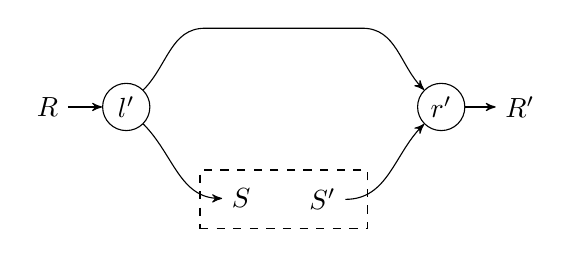
\begin{tikzpicture}
\node[vert] (l) at (0, 0) {$l'$};
\node[vert] (r) at (4, 0) {$r'$};

\node (R) [left of=l] {$R$};
\node (S) [below right = 0.7 and 1 of l] {$S$};
\node (R') [right of=r] {$R'$};
\node (S') [below left = 0.7 and 1 of r] {$S'$};

\draw[->] (R) -- (l);
\draw[->] (l) to[out=south east,in=west] (S);

\draw[<-] (R') -- (r);
\draw[<-] (r) to[out=south west,in=east] (S');

\draw[->] (l) to[out=north east, in=west] ++(1,1)
 to ++(2,0)
 to[out=east, in=north west] (r)
;

\node[draw,dashed,fit=(S) (S'), inner xsep = 8pt] (box) {};
\end{tikzpicture} \\
  \raisebox{1.5cm}{$:=$}\qquad
  \begin{tikzpicture}
\begin{scope}[on grid]

\node[vert] (l') at (0, 0) {$l'$};
\node[vert, below right = 0.7 and 1 of l'] (l) {$l$};
\node[vert] (r') at (5, 0) {$r'$};
\node[vert, below left = 0.7 and 1 of r'] (r) {$r$};

\node (A) [below right = 0.7 and 1 of l] {$A$};
\node (A') [below left = 0.7 and 1 of r] {$A'$};

\node (R) [left of=l'] {$R$};
\node (R') [right of=r'] {$R'$};

\draw[->] (R) -- (l');
\draw[<-] (R') -- (r');

\draw[->] (l') to[rrel, out=north east, in=west] (1,1)
 to +(3,0)
 to[out=east, in=north west] (r')
;

\draw[->] (l) to[rrel, out=north east, in=west] (1,1)
 to +(1,0)
 to[out=east, in=north west] (r)
;

\draw[->] (l') to[out=south east,in=west] (l);
\draw[->] (r) to[out=east, in=south west] (r');

\draw[->] (l) to[out=south east,in=west] (A);
\draw[<-] (r) to[out=south west,in=east] (A');

\node[draw,dashed,fit=(l) (r), inner xsep = 6pt, inner ysep = 25pt] (box2) {};
\node[draw,dashed,fit=(A) (A'), inner xsep = 8pt] (box) {};
\end{scope}
\end{tikzpicture}
\end{center}

The identity optic $(S, S') \hto (S, S')$ is given by $\rep{\lambda^{-1}_S}{\lambda_{S'}}$, where $\lambda_S : I \otimes S \to S$ is the left unitor for $S$:
\begin{center}
  \begin{tikzpicture}
\begin{scope}[on grid]
\node[vert] (l) at (0, 0) {$\lambda_S^{-1}$};
\node[vert] (r) at (4, 0) {$\lambda_{S'}$};

\node (S) [left of=l] {$S$};
\node (A) [below right = 0.7 and 1 of l] {$S$};
\node (S') [right of=r] {$S'$};
\node (A') [below left = 0.7 and 1 of r] {$S'$};

\draw[->] (S) -- (l);
\draw[->] (l) to[out=south east,in=west] (A);

\draw[<-] (S') -- (r);
\draw[<-] (r) to[out=south west,in=east] (A');

\draw[->, dotted] (l) to[rrel, out=north east, in=west] (1,1)
 to +(2,0)
 to[out=east, in=north west] (r)
;

\node[draw,dashed,fit=(A) (A'), inner xsep = 8pt] (box) {};
\end{scope}
\end{tikzpicture}
\end{center}
This dashed line above the diagram represents the unit object. It is common in string diagrams to omit unitors and the unit object unless they are necessary to make sense of the diagram. In this case, we would draw:
\begin{center}
  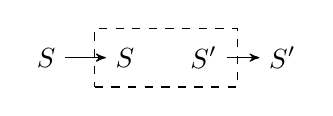
\begin{tikzpicture}
\node (Sin) {$S$};
\node (Sout) [right of=Sin] {$S$};
\node (Spout) [right of=Sout] {$S'$};
\node (Spin) [right of=Spout] {$S'$};

\draw[->] (Sin) -- (Sout);
\draw[->] (Spout) -- (Spin);

\node[draw,dashed,fit=(Sout) (Spout), inner xsep = 4pt] (box) {};
\end{tikzpicture}
\end{center}

\begin{proposition}\label{prop-optic-is-cat}
  The above data form a category $\Optic_\otimes$.
\end{proposition}
\begin{proof}
  In~\cite[Section 6]{Doubles} this is proven abstractly, by exhibiting this category as the Kleisli category for a monad in the bicategory $\Prof$. Here we prove the conditions directly.

  We check associativity of composition equationally.  Suppose we have representatives of three optics $\rep{l_1}{r_1} : (R, R) \hto (S, S')$, $\rep{l_2}{r_2} : (S, S') \hto (A, A')$ and $\rep{l_3}{r_3} : (A, A') \hto (B, B')$, that have residuals $M$, $N$ and $P$ respectively. As in the definition of composition, the Fubini theorem for coends allows us to choose these representatives simultaneously. Then:
  \begin{align*}
    (\rep{l_3}{r_3} \circ \rep{l_2}{r_2}) \circ \rep{l_1}{r_1}
    &= \rep{(N \otimes l_3)l_2}{r_2(N \otimes r_3)} \circ \rep{l_1}{r_1} \\
    &= \rep{(M \otimes ((N \otimes l_3)l_2))l_1}{r_1(M \otimes (r_2(N \otimes r_3)))} \\
    &= \rep{(M \otimes N \otimes l_3)(M \otimes l_2)l_1}{r_1(M \otimes r_2)(M \otimes N \otimes r_3)} \\
    &= \rep{l_3}{r_3} \circ (\rep{(M \otimes l_2)l_1}{r_1(M \otimes r_2)}) \\
    &= \rep{l_3}{r_3} \circ (\rep{l_2}{r_2} \circ \rep{l_1}{r_1})
  \end{align*}

  For the unit laws, suppose we have $\rep{l}{r} : (S, S') \hto (A, A')$ with representative $M$. We calculate:
  \begin{align*}
    \id_{A, A'} \circ \rep{l}{r}
    &= \rep{\lambda^{-1}_A}{\lambda_{A'}} \circ \rep{l}{r} \\
    &= \rep{(M \otimes \lambda^{-1}_A) l}{r (M\otimes  \lambda_{A'}} \\
    &= \rep{(\rho^{-1}_M \otimes  A) l}{r (\rho_M \otimes A'} \\
    &= \rep{l}{r (\rho_M \otimes A') (\rho^{-1}_M \otimes A')} \\
    &= \rep{l}{r} \\
    \rep{l}{r} \circ \id_{S, S'}
    &= \rep{l}{r} \circ \rep{\lambda^{-1}_S}{\lambda_{S'}}  \\
    &= \rep{(I \otimes l)\lambda^{-1}_S}{\lambda_{S'} (I \otimes r)} \\
    &= \rep{(\lambda^{-1}_M \otimes S)l}{r (\lambda_{M} \otimes S')} \\
    &= \rep{l}{r (\lambda_{M} \otimes S')(\lambda^{-1}_M \otimes S')} \\
    &= \rep{l}{r}
  \end{align*}
  In both cases we have used the naturality of $\lambda$ followed by the coend relations to move $\lambda^{-1}_M$ to the right-hand side, where it may be cancelled with $\lambda_M$
\end{proof}

\begin{remark}
  Note that the hom-sets of $\Optic_\otimes$ are given by a coend indexed by a possibly large category, so their existence is not guaranteed by the cocompleteness of $\Set$. We should be careful to only discuss $\Optic$ categories where we know that the coends exist by some other means, e.g., by exhibiting an isomorphism with some other set. For all of the examples given later, we provide such an isomorphism.
\end{remark}

The remainder of this section comprises some useful observations that were not made in~\cite{Doubles}.

\begin{proposition}
  There is a functor $\iota : \C \times \C^\op \to \Optic_\otimes$, which is given on objects by $\iota(S, S') = (S, S')$ and for a morphism $(f, g) : (S, S') \to (A, A')$ by $\iota(f, g) = \rep{\lambda_A^{-1} f}{g \lambda_{A'}}$.
\end{proposition}
\begin{proof}
  Graphically, this is:
  \begin{center}
    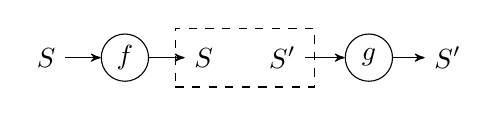
\begin{tikzpicture}
\node (Sin) {$S$};
\node (f) [vert, right of=Sin] {$f$};
\node (Sout) [right of=f] {$S$};
\node (Spout) [right of=Sout] {$S'$};
\node (g) [vert, right = 0.5 of Spout] {$g$};
\node (Spin) [right of=g] {$S'$};

\draw[->] (Sin) -- (f);
\draw[->] (f) -- (Sout);
\draw[->] (Spout) -- (g);
\draw[->] (g) -- (Spin);

\node[draw,dashed,fit=(Sout) (Spout)] (box) {};
\end{tikzpicture}
  \end{center}

  This preserves identities, as the identity on an object $(S, S')$ in $\Optic_\otimes$ is defined to be exactly $\rep{\lambda^{-1}_S}{\lambda_{S'}}$. To check functoriality, suppose we have $(f, g) : (S, S') \to (A, A')$ and $(f', g') : (A, A') \to (B, B')$ in $\C \times \C^\op$. Then:
  \begin{align*}
    \iota(f', g') \circ \iota(f, g)
    &= \rep{\lambda^{-1}_B f'}{g' \lambda_{B'}} \circ \rep{\lambda^{-1}_A f}{g \lambda_{A'}} \\
    &= \rep{(I\otimes (\lambda^{-1}_B f'))\lambda^{-1}_A f}{g \lambda_{A'} (I\otimes (g' \lambda_{B'})} && \text{(By definition of $\circ$)}\\
    &= \rep{(I \otimes \lambda^{-1}_B) (I \otimes f')\lambda^{-1}_A f}{g \lambda_{A'} (I \otimes g')(I\otimes \lambda_{B'}} && \text{(Functoriality of $I \otimes -$)}\\
    &= \rep{(I\otimes \lambda^{-1}_B) \lambda^{-1}_B f' f}{g g' \lambda_{B'} (I\otimes \lambda_{B'}} && \text{(Naturality of $\lambda$)}\\
    &= \rep{(\lambda^{-1}_I \otimes B) \lambda^{-1}_B f' f}{g g' \lambda_{B'} (\lambda_I \otimes B'} && \text{(Unitality of action)} \\
    &= \rep{\lambda^{-1}_B f' f}{g g' \lambda_{B'} (\lambda_I \otimes B') (\lambda^{-1}_I \otimes B')} && \text{(Coend relation)}  \\
    &= \rep{\lambda^{-1}_B f'f}{g g' \lambda_{B'}} \\
    &= \iota(f'f, gg')
  \end{align*}
  Graphically, there is not much to do:
  \begin{center}
    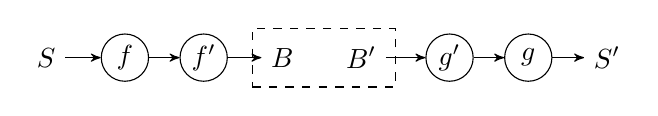
\begin{tikzpicture}
\node (Sin) {$S$};
\node (f) [vert, right of=Sin] {$f$};
\node (f') [vert, right of=f] {$f'$};
\node (Sout) [right of=f'] {$B$};
\node (Spout) [right of=Sout] {$B'$};
\node (g') [vert, right = 0.5 of Spout] {$g'$};
\node (g) [vert, right of=g'] {$g$};
\node (Spin) [right of=g] {$S'$};

\draw[->] (Sin) -- (f);
\draw[->] (f) -- (f');
\draw[->] (f') -- (Sout);
\draw[->] (Spout) -- (g');
\draw[->] (g') -- (g);
\draw[->] (g) -- (Spin);

\node[draw,dashed,fit=(Sout) (Spout)] (box) {};
\end{tikzpicture}
    \qquad \raisebox{0.3cm}{$=$} \qquad
    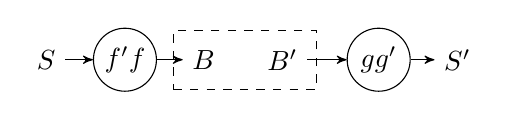
\begin{tikzpicture}
\node (Sin) {$S$};
\node (f) [vertbig, right of=Sin] {$f'f$};
\node (Sout) [right of=f] {$B$};
\node (Spout) [right of=Sout] {$B'$};
\node (g) [vertbig, right = 0.5 of Spout] {$gg'$};
\node (Spin) [right of=g] {$S'$};

\draw[->] (Sin) -- (f);
\draw[->] (f) -- (Sout);
\draw[->] (Spout) -- (g);
\draw[->] (g) -- (Spin);

\node[draw,dashed,fit=(Sout) (Spout)] (box) {};
\end{tikzpicture}
  \end{center}

\end{proof}

\begin{remark}
  This functor is not necessarily faithful, see Remark~\ref{lens-iota-not-faithful}.
\end{remark}

% \todo{This doesn't give us the structure of a `framing', we can only lift vertical arrows to horizontal arrows facing one direction.}

% \begin{theorem}
%   $\Optic_\otimes$ is symmetric monoidal, where $(S, S') \otimes (T, T') = (S \otimes T, S' \otimes T')$, the unit is $(I, I)$, and the action on morphisms induced by
%   \begin{align*}
%     &\C(S, M \otimes A) \times \C(M \otimes A', S') \times \C(T, N \otimes B) \times \C(N \otimes B', T')\\
%     \to \quad&\C(S \otimes T, M \otimes A \otimes N \otimes B) \times \C(M \otimes A' \otimes N \otimes B', S' \otimes T') && \text{(action of $\otimes$ on morphisms in $\C$)}\\
%     \to \quad&\C(S \otimes T, M \otimes N \otimes A \otimes B) \times \C(M \otimes N \otimes A' \otimes B', S' \otimes T') && \text{($\otimes$ in $\C$ is symmetric)}\\
%     \to \quad&\int^{M \in \C} \C(S \otimes T, M \otimes A \otimes B) \times \C(M \otimes A' \otimes B', S' \otimes T') && \text{(inclusion into coend)}
%   \end{align*}
% \end{theorem}
% \begin{proof}
%   Equationally, suppose we have representatives $(l, r) : (S \to M \otimes A, M \otimes A' \to S')$ and $(l', r') : (T \to N \otimes B, N \otimes B' \to T')$. Then:
%   \begin{align*}
%     \langle l, r \rangle \otimes \langle l', r' \rangle &:= \langle (M \otimes s_{A,N} \otimes B)(l \otimes l'), (r \otimes r')(M \otimes s_{A',N} \otimes B') \rangle
%   \end{align*}
%   This is functorial, as suggested by the equivalence of the following string diagrams:
%   \todo{todo}
%%   For future convenience, note that
%%   \begin{align*}
%%     \langle l, r \rangle \otimes (T, T') &= \langle (M \otimes s_{A,I} \otimes T)(l \otimes \lambda_T), (r \otimes \lambda^{-1}_{T'})(M \otimes s_{A',I}\otimes T') \rangle \\
%%     &= \langle (\lambda^{-1}_M \otimes A \otimes T)(M \otimes s_{A,I} \otimes T)(l \otimes \lambda_T), (r \otimes \lambda^{-1}_{T'})(M \otimes s_{A',I}\otimes T')(\lambda_M \otimes A' \otimes T') \rangle \\
%%     &= \langle l \otimes T, r \otimes T' \rangle
%%   \end{align*}
%%   Now we check functoriality. Suppose we have:
%%   \begin{align*}
%%     \langle l_1, r_1 \rangle : (S_1, S_1') &\hto (S_2, S_2') \\
%%     \langle l_2, r_2 \rangle : (S_2, S_2') &\hto (S_3, S_3') \\
%%     \langle p_1, q_1 \rangle : (T_1, T_1') &\hto (T_2, T_2') \\
%%     \langle p_2, q_2 \rangle : (T_2, T_2') &\hto (T_3, T_3')
%%   \end{align*}
%%   with residuals $M_1, M_2, N_1, N_2$ respectively. Then: \todo {(This is a mess. String diagram?)}
%%   \begin{align*}
%%     &(\langle l_2, r_2 \rangle \otimes \langle p_2, q_2 \rangle) \circ (\langle l_1, r_1 \rangle \otimes \langle p_1, q_1 \rangle) \\
%%     = \; &\langle (M_2 \otimes s_{S_3,N_2} \otimes T_3)(l_2 \otimes p_2), (r_2 \otimes q_2)(M_2 \otimes s_{S_3',N_2} \otimes T_3') \rangle \\
%%     &\circ \langle (M_1 \otimes s_{S_2,N_1} \otimes T_2)(l_1 \otimes p_1), (r_1 \otimes q_1)(M_1 \otimes s_{S_2',N_1} \otimes T_2') \rangle \\
%%     = \; & \langle (M_1 \otimes N_1 \otimes M_2 \otimes s_{S_3,N_2} \otimes T_3)(M_1 \otimes N_1 \otimes l_2 \otimes p_2)(M_1 \otimes s_{S_2,N_1} \otimes T_2)(l_1 \otimes p_1), \\
%%     &\;(r_1 \otimes q_1)(M_1 \otimes s_{S_2',N_1} \otimes T_2')(M_1 \otimes N_1 \otimes r_2 \otimes q_2)(M_1 \otimes N_1 \otimes M_2 \otimes s_{S_3',N_2} \otimes T_3') \rangle \\
%%     = \; & \langle (M_1 \otimes N_1 \otimes M_2 \otimes s_{S_3,N_2} \otimes T_3)(M_1 \otimes s_{(M_2 \otimes S_3),N_1} \otimes T_3)(M_1 \otimes  l_2 \otimes N_1 \otimes p_2)(l_1 \otimes p_1), \\
%%     &\;(r_1 \otimes q_1)(M_1 \otimes r_2 \otimes N_1 \otimes q_2)(M_1 \otimes s_{(M_2 \otimes S_3'),N_1} \otimes T_3')(M_1 \otimes N_1 \otimes M_2 \otimes s_{S_3',N_2} \otimes T_3') \rangle \\
%%     = \; & \langle (M_1 \otimes N_1 \otimes M_2 \otimes s_{S_3,N_2} \otimes T_3)(M_1 \otimes s_{(M_2 \otimes S_3),N_1} \otimes T_3)((M_1 \otimes l_2)l_1\otimes (N_1 \otimes p_2)p_1), \\
%%     &\;(r_1(M_1 \otimes r_2) \otimes q_1(N_1 \otimes q_2))(M_1 \otimes s_{(M_2 \otimes S_3'),N_1} \otimes T_3')(M_1 \otimes N_1 \otimes M_2 \otimes s_{S_3',N_2} \otimes T_3') \rangle \\
%%     = \; & \text{\todo{(Add a $s_{M_2, N_1}$ to either side of the coend, then appeal to coherence)}} \\
%%     = \; &\langle (M_1 \otimes M_2 \otimes s_{(N_1 \otimes N_2),S_3} \otimes T_3)((M_1 \otimes l_2)l_1\otimes (N_1 \otimes p_2)p_1) ,  \\
%%     &\;(r_1(M_1 \otimes r_2) \otimes q_1(N_1 \otimes q_2))(M_1 \otimes M_2 \otimes s_{(N_1 \otimes N_2),S'_3} \otimes T'_3) \rangle \\
%%     = \; &\langle (M_1 \otimes l_2)l_1, r_1(M_1 \otimes r_2) \rangle \otimes \langle (N_1 \otimes p_2)p_1, q_1(N_1 \otimes q_2) \rangle \\
%%     = \; &(\langle l_2, r_2 \rangle  \circ \langle l_1, r_1 \rangle) \otimes (\langle p_2, q_2 \rangle \circ \langle p_1, q_1 \rangle)
%%   \end{align*}
%
%   The structure morphisms are all lifted from the structure morphisms in $\C$:
%   \begin{align*}
%     \alpha_{(R, R'), (S, S'), (T, T')} &:= \iota(\alpha_{R,S,T}, \alpha_{R',S',T'}^{-1}) \\
%     \lambda_{(S, S')} &:= \iota(\lambda_{(S, S')}, \lambda_{(S, S')}^{-1}) \\
%     \rho_{(S, S')} &:= (\rho_{(S, S')}, \rho_{(S, S')}^{-1}) \\
%     s_{(S, S'), (T, T')} &:= \iota(s_{S, T}, s_{T', S'})
%   \end{align*}
%
%   Note that because $\iota(S, S') = (S, S')$, required equations for $\iota$ to be a monoidal functor hold by definition (although we don't yet know that $\Optic_\otimes$ is monoidal). The pentagon and triangle axioms then hold in $\Optic_\otimes$, as they are the image of the same axioms in $\C \times \C^\op$ under $\iota$. The only remaining thing to verify is that these structure maps are natural in $\Optic_\otimes$.
%
%   Let us check that $\alpha_{(R, R'), (S, S'), (T, T')}$ is natural in $(R, R')$. Suppose $f : (Q, Q') \hto (R, R')$ has representative $(l, r) : (Q \to M \otimes R, M \otimes R' \to Q')$, then:
%   \begin{align*}
%     &\alpha_{(R, R'), (S, S'), (T, T')} \circ (f \otimes (S, S')) \otimes (T, T') \\
%     &= \iota(\alpha_{R,S,T}, \alpha_{R',S',T'}^{-1})  \circ (\langle l, r \rangle \otimes (S, S')) \otimes (T, T') \\
%     &= \langle\lambda_{R \otimes (S \otimes T)}\alpha_{R,S,T}, \alpha_{R',S',T'}^{-1} \lambda^{-1}_{(R' \otimes S') \otimes T'} \rangle  \circ \left\langle (l \otimes S) \otimes T, (r \otimes S') \otimes T' \right\rangle \\
%     &=\left\langle (M \otimes \lambda_{R \otimes (S \otimes T)}\alpha_{R,S,T})((l \otimes S) \otimes T), ((r \otimes S') \otimes T') (M \otimes \alpha_{R',S',T'}^{-1} \lambda^{-1}_{(R' \otimes S') \otimes T'} ) \right\rangle \\
%     &=\left\langle (M \otimes \alpha_{R,S,T})((l \otimes S) \otimes T), ((r \otimes S') \otimes T') (M \otimes \alpha_{R',S',T'}^{-1} )\right\rangle \\
%     &=\left\langle (l \otimes (S \otimes T))\alpha_{Q,S,T}, \alpha_{Q',S',T'}^{-1}(r \otimes (S' \otimes T')) \right\rangle \\
%     &= \langle (I \otimes l \otimes (S \otimes T)) \lambda_{Q \otimes (S \otimes T)}\alpha_{Q,S,T}, (I \times r \otimes (S' \otimes T')) \alpha_{Q',S',T'}^{-1} \lambda^{-1}_{Q' \otimes (S' \otimes T')}\rangle \\
%     &= \langle l \otimes (S \otimes T), r \otimes (S' \otimes T')\rangle \circ \left\langle \lambda_{Q \otimes (S \otimes T)}\alpha_{Q,S,T}, \alpha_{Q',S',T'}^{-1} \lambda^{-1}_{Q' \otimes (S' \otimes T')} \right\rangle \\
%     &= \langle l, r \rangle \otimes ((S, S') \otimes (T, T')) \circ \iota(\alpha_{Q,S,T}, \alpha_{Q',S',T'}^{-1}) \\
%     &= f \otimes ((S, S') \otimes (T, T')) \circ \alpha_{(Q, Q'), (S, S'), (T, T')}
%   \end{align*}
%   \todo{There is some cheating going on here, composition actually adds an extra $\alpha$, but that wouldn't get in the way.}
% \end{proof}

\begin{theorem}
  $\Optic_\otimes$ is symmetric monoidal, where $(S, S') \otimes (T, T') = (S \otimes T, S' \otimes T')$, the unit object is $(I, I)$, and the action on a pair of morphisms $\rep{l}{r} : S \hto A$ and $\rep{l'}{r'} : T \hto B$ is given by:
  \begin{center}
    \begin{tikzpicture}
\begin{scope}[on grid]

\node[vert] (l) at (0, 0) {$l$};
\node[vert] (r) at (6, 0) {$r$};

\node (S) [left of=l] {$S$};
\node (A) [below right = 2 and 2 of l] {$A$};
\node (S') [right of=r] {$S'$};
\node (A') [below left = 2 and 2 of r] {$A'$};

\draw[->] (S) -- (l);
\draw[->] (l) to[out=south east,in=west] (A);

\draw[<-] (S') -- (r);
\draw[<-] (r) to[out=south west,in=east] (A');

\draw[->] (l) to[rrel, out=north east, in=west] (1,1)
 to ++(4,0)
 to[out=east, in=north west] (r)
;

\node[vert] (l') at (0, -2) {$l'$};
\node[vert] (r') at (6, -2) {$r'$};

\node (T) [left of=l'] {$T$};
\node (B) [below right = 1 and 2 of l'] {$B$};
\node (T') [right of=r'] {$T'$};
\node (B') [below left = 1 and 2 of r'] {$B'$};

\draw[->] (T) -- (l');
\draw[->] (l') to[out=south east,in=west] (B);

\draw[<-] (T') -- (r');
\draw[<-] (r') to[out=south west,in=east] (B');

\draw[->] (l') 
 to[rrel, out=north east, in=west] (2,2)
 to ++(2,0)
 to[out=east, in=north west] (r')
;

\node[draw,dashed,fit=(A) (A') (B) (B'), inner xsep = 8pt] (box) {};

\end{scope}
\end{tikzpicture}
  \end{center}
\end{theorem}
\begin{proof}
  Suppose the two optics have residuals $M$ and $N$ respectively. Written equationally, their tensor is:
  \begin{align*}
    \rep{l}{r} \otimes \rep{l'}{r'} &:= \rep{(M \otimes s_{A,N} \otimes B)(l \otimes l')}{(r \otimes r')(M \otimes s_{A',N} \otimes B')}
  \end{align*}
  This is well-defined, as the calculus of string diagrams allows us to combine the coend relation on each optic to establish the coend relation for the compound diagram. \todo{draw this?}

  Let us check functoriality of $\otimes$. Suppose we have optics:
  \begin{align*}
    \rep{l_1}{r_1} : (S_1, S_1') &\hto (S_2, S_2') \\
    \rep{l_2}{r_2} : (S_2, S_2') &\hto (S_3, S_3') \\
    \rep{p_1}{q_1} : (T_1, T_1') &\hto (T_2, T_2') \\
    \rep{p_2}{q_2} : (T_2, T_2') &\hto (T_3, T_3')
  \end{align*}
  The string diagram for $(\rep{l_2}{r_2} \circ \rep{l_1}{r_1}) \otimes (\rep{p_2}{q_2} \circ \rep{p_1}{q_1})$ is:
  \begin{center}
    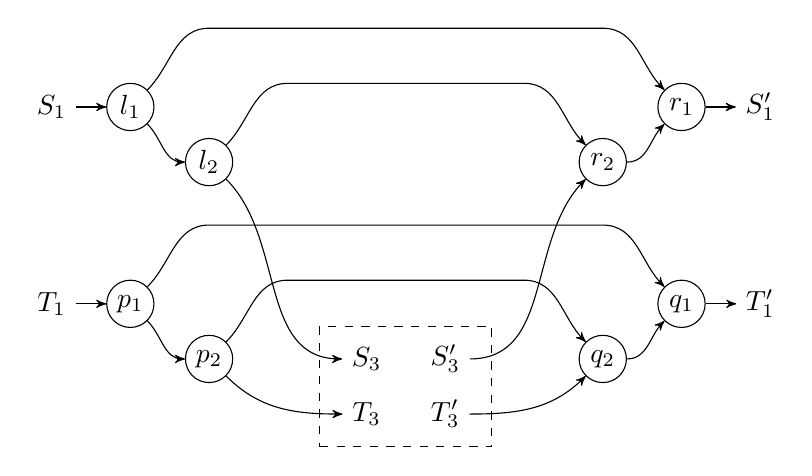
\begin{tikzpicture}
\begin{scope}[on grid]

%%% The S part

\node[vert] (l1) at (0, 0) {$l_1$};
\node[vert, below right = 0.7 and 1 of l1] (l2) {$l_2$};
\node[vert] (r1) at (7, 0) {$r_1$};
\node[vert, below left = 0.7 and 1 of r1] (r2) {$r_2$};

\node (S3) [below right = 2.5 and 2 of l2] {$S_3$};
\node (S3') [below left = 2.5 and 2 of r2] {$S_3'$};

\node (S1) [left of=l1] {$S_1$};
\node (S1') [right of=r1] {$S_1'$};

\draw[->] (S1) -- (l1);
\draw[<-] (S1') -- (r1);

\draw[->] (l1) to[out=north east, in=west] ++(1,1)
 to ($(r1) + (-1,1)$)
 to[out=east, in=north west] (r1)
;

\draw[->] (l2) to[out=north east, in=west] ++(1,1)
 to ($(r2) + (-1,1)$)
 to[out=east, in=north west] (r2)
;

\draw[->] (l1) to[out=south east,in=west] (l2);
\draw[->] (r2) to[out=east, in=south west] (r1);

\draw[->] (l2) to[out=south east,in=west] (S3);
\draw[<-] (r2) to[out=south west,in=east] (S3');

%%% The T part

\node[vert] (p1) at (0, -2.5) {$p_1$};
\node[vert, below right = 0.7 and 1 of p1] (p2) {$p_2$};
\node[vert] (q1) at (7, -2.5) {$q_1$};
\node[vert, below left = 0.7 and 1 of q1] (q2) {$q_2$};

\node (T3) [below right = 0.7 and 2 of p2] {$T_3$};
\node (T3') [below left = 0.7 and 2 of q2] {$T_3'$};

\node (T1) [left of=p1] {$T_1$};
\node (T1') [right of=q1] {$T_1'$};

\draw[->] (T1) -- (p1);
\draw[<-] (T1') -- (q1);

\draw[->] (p1) 
 to[out=north east, in=west] ++(1,1)
 to ($(q1) + (-1,1)$)
 to[out=east, in=north west] (q1)
;

\draw[->] (p2) to[out=north east, in=west] ++(1,1)
 to ($(q2) + (-1,1)$)
 to[out=east, in=north west] (q2)
;

\draw[->] (p1) to[out=south east,in=west] (p2);
\draw[->] (q2) to[out=east, in=south west] (q1);

\draw[->] (p2) to[out=south east,in=west] (T3);
\draw[<-] (q2) to[out=south west,in=east] (T3');

\node[draw,dashed,fit=(S3) (S3') (T3) (T3'), inner xsep = 8pt] (box) {};

\end{scope}
\end{tikzpicture}
  \end{center}
  And for $(\rep{l_2}{r_2} \otimes \rep{p_2}{q_2}) \circ (\rep{l_1}{r_1} \otimes \rep{p_1}{q_1})$ is:
  \begin{center}
    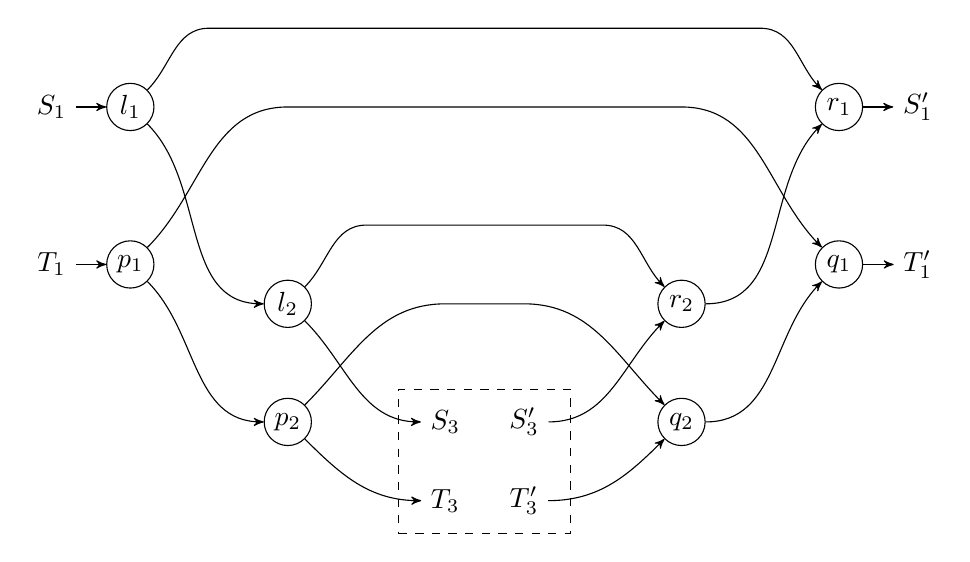
\begin{tikzpicture}
\begin{scope}[on grid]

%%% Outer:

\node[vert] (l1) at (0, 0) {$l_1$};
\node[vert] (r1) at (9, 0) {$r_1$};

\node (S1) [left of=l1] {$S_1$};
\node[vert] (l2) [below right = 2.5 and 2 of l1] {$l_2$};
\node (S1') [right of=r1] {$S_1'$};
\node[vert] (r2) [below left = 2.5 and 2 of r1] {$r_2$};

\draw[->] (S1) -- (l1);
\draw[->] (l1) to[out=south east,in=west] (l2);

\draw[<-] (S1') -- (r1);
\draw[<-] (r1) to[out=south west,in=east] (r2);

\draw[->] (l1) to[out=north east, in=west] ++(1,1)
 to ($(r1) + (-1,1)$)
 to[out=east, in=north west] (r1)
;

\node[vert] (p1) at (0, -2) {$p_1$};
\node[vert] (q1) at (9, -2) {$q_1$};

\node (T1) [left of=p1] {$T_1$};
\node[vert] (p2) [below right = 2 and 2 of p1] {$p_2$};
\node (T') [right of=q1] {$T_1'$};
\node[vert] (q2) [below left = 2 and 2 of q1] {$q_2$};

\draw[->] (T1) -- (p1);
\draw[->] (p1) to[out=south east,in=west] (p2);

\draw[<-] (T') -- (q1);
\draw[<-] (q1) to[out=south west,in=east] (q2);

\draw[->] (p1) 
 to[out=north east, in=west] ++(2,2)
 to ($(q1) + (-2,2)$)
 to[out=east, in=north west] (q1)
;

%%% Inner:

\draw[->] (l2) to[out=north east, in=west] ++(1,1)
 to ($(r2) + (-1,1)$)
 to[out=east, in=north west] (r2)
;
\draw[->] (p2) 
 to[out=north east, in=west] ++(2,1.5)
 to ($(q2) + (-2,1.5)$)
 to[out=east, in=north west] (q2)
;

\node(S3) [below right = 1.5 and 2 of l2] {$S_3$};
\node(S3') [below left = 1.5 and 2 of r2] {$S_3'$};

\draw[->] (l2) to[out=south east,in=west] (S3);
\draw[<-] (r2) to[out=south west,in=east] (S3');

\node (T3) [below right = 1 and 2 of p2] {$T_3$};
\node (T3') [below left = 1 and 2 of q2] {$T_3'$};

\draw[->] (p2) to[out=south east,in=west] (T3);
\draw[<-] (q2) to[out=south west,in=east] (T3');


\node[draw,dashed,fit=(S3) (S3') (T3) (T3'), inner xsep = 8pt] (box) {};
the a
\end{scope}
\end{tikzpicture}
  \end{center}
  These two diagrams are equivalent: We can use the naturality of the symmetry morphism to push $l_2$ and $r_2$ past the crossing to be next to $l_1$ and $r_1$ respectively. This creates two extra twists that can be cancelled in the center of the diagram (implicitly using the coend relation).

  %%%% Note: The following is the above argument written equationally:
  % For future convenience, note that
  % \begin{align*}
  %   \langle l, r \rangle \otimes (T, T') &= \langle (M \otimes s_{A,I} \otimes T)(l \otimes \lambda_T), (r \otimes \lambda^{-1}_{T'})(M \otimes s_{A',I}\otimes T') \rangle \\
  %   &= \langle (\lambda^{-1}_M \otimes A \otimes T)(M \otimes s_{A,I} \otimes T)(l \otimes \lambda_T), (r \otimes \lambda^{-1}_{T'})(M \otimes s_{A',I}\otimes T')(\lambda_M \otimes A' \otimes T') \rangle \\
  %   &= \langle l \otimes T, r \otimes T' \rangle
  % \end{align*}
  % Now we check functoriality. Suppose we have:
  % \begin{align*}
  %   \langle l_1, r_1 \rangle : (S_1, S_1') &\hto (S_2, S_2') \\
  %   \langle l_2, r_2 \rangle : (S_2, S_2') &\hto (S_3, S_3') \\
  %   \langle p_1, q_1 \rangle : (T_1, T_1') &\hto (T_2, T_2') \\
  %   \langle p_2, q_2 \rangle : (T_2, T_2') &\hto (T_3, T_3')
  % \end{align*}
  % with residuals $M_1, M_2, N_1, N_2$ respectively. Then: \todo {(This is a mess. String diagram?)}
  % \begin{align*}
  %   &(\langle l_2, r_2 \rangle \otimes \langle p_2, q_2 \rangle) \circ (\langle l_1, r_1 \rangle \otimes \langle p_1, q_1 \rangle) \\
  %   = \; &\langle (M_2 \otimes s_{S_3,N_2} \otimes T_3)(l_2 \otimes p_2), (r_2 \otimes q_2)(M_2 \otimes s_{S_3',N_2} \otimes T_3') \rangle \\
  %   &\circ \langle (M_1 \otimes s_{S_2,N_1} \otimes T_2)(l_1 \otimes p_1), (r_1 \otimes q_1)(M_1 \otimes s_{S_2',N_1} \otimes T_2') \rangle \\
  %   = \; & \langle (M_1 \otimes N_1 \otimes M_2 \otimes s_{S_3,N_2} \otimes T_3)(M_1 \otimes N_1 \otimes l_2 \otimes p_2)(M_1 \otimes s_{S_2,N_1} \otimes T_2)(l_1 \otimes p_1), \\
  %   &\;(r_1 \otimes q_1)(M_1 \otimes s_{S_2',N_1} \otimes T_2')(M_1 \otimes N_1 \otimes r_2 \otimes q_2)(M_1 \otimes N_1 \otimes M_2 \otimes s_{S_3',N_2} \otimes T_3') \rangle \\
  %   = \; & \langle (M_1 \otimes N_1 \otimes M_2 \otimes s_{S_3,N_2} \otimes T_3)(M_1 \otimes s_{(M_2 \otimes S_3),N_1} \otimes T_3)(M_1 \otimes  l_2 \otimes N_1 \otimes p_2)(l_1 \otimes p_1), \\
  %   &\;(r_1 \otimes q_1)(M_1 \otimes r_2 \otimes N_1 \otimes q_2)(M_1 \otimes s_{(M_2 \otimes S_3'),N_1} \otimes T_3')(M_1 \otimes N_1 \otimes M_2 \otimes s_{S_3',N_2} \otimes T_3') \rangle \\
  %   = \; & \langle (M_1 \otimes N_1 \otimes M_2 \otimes s_{S_3,N_2} \otimes T_3)(M_1 \otimes s_{(M_2 \otimes S_3),N_1} \otimes T_3)((M_1 \otimes l_2)l_1\otimes (N_1 \otimes p_2)p_1), \\
  %   &\;(r_1(M_1 \otimes r_2) \otimes q_1(N_1 \otimes q_2))(M_1 \otimes s_{(M_2 \otimes S_3'),N_1} \otimes T_3')(M_1 \otimes N_1 \otimes M_2 \otimes s_{S_3',N_2} \otimes T_3') \rangle \\
  %   = \; & \text{\todo{(Add a $s_{M_2, N_1}$ to either side of the coend, then appeal to coherence)}} \\
  %   = \; &\langle (M_1 \otimes M_2 \otimes s_{(N_1 \otimes N_2),S_3} \otimes T_3)((M_1 \otimes l_2)l_1\otimes (N_1 \otimes p_2)p_1) ,  \\
  %   &\;(r_1(M_1 \otimes r_2) \otimes q_1(N_1 \otimes q_2))(M_1 \otimes M_2 \otimes s_{(N_1 \otimes N_2),S'_3} \otimes T'_3) \rangle \\
  %   = \; &\langle (M_1 \otimes l_2)l_1, r_1(M_1 \otimes r_2) \rangle \otimes \langle (N_1 \otimes p_2)p_1, q_1(N_1 \otimes q_2) \rangle \\
  %   = \; &(\langle l_2, r_2 \rangle  \circ \langle l_1, r_1 \rangle) \otimes (\langle p_2, q_2 \rangle \circ \langle p_1, q_1 \rangle)
  % \end{align*}

  The structure morphisms are all lifted from the structure morphisms in $\C \times \C^\op$:
  \begin{align*}
    \alpha_{(R, R'), (S, S'), (T, T')} &:= \iota(\alpha_{R,S,T}, \alpha_{R',S',T'}^{-1}) \\
    \lambda_{(S, S')} &:= \iota(\lambda_{S}, \lambda_{S'}^{-1}) \\
    \rho_{(S, S')} &:= \iota(\rho_{S}, \rho_{S'}^{-1}) \\
    s_{(S, S'), (T, T')} &:= \iota(s_{S, T}, s_{T', S'})
  \end{align*}

  Note that because $\iota(S, S') = (S, S')$, required equations for $\iota$ to be a monoidal functor hold by definition (although we don't yet know that $\Optic_\otimes$ is monoidal). The pentagon and triangle equations then hold in $\Optic_\otimes$, as they are the image of the same axioms in $\C \times \C^\op$ under $\iota$. The only remaining thing to verify is that these structure maps are natural in $\Optic_\otimes$.

  Let us check that $\alpha_{(R, R'), (S, S'), (T, T')}$ is natural in $(R, R')$. Suppose $\rep{l}{r} : (Q, Q') \hto (R, R')$ is an optic with residual $M$.
  \begin{align*}
    &\alpha_{(R, R'), (S, S'), (T, T')} \circ (f \otimes (S, S')) \otimes (T, T') \\
    &= \iota(\alpha_{R,S,T}, \alpha_{R',S',T'}^{-1})  \circ (\rep{l}{r} \otimes (S, S')) \otimes (T, T') \\
    &= \rep{\lambda_{R \otimes (S \otimes T)}\alpha_{R,S,T}}{\alpha_{R',S',T'}^{-1} \lambda^{-1}_{(R' \otimes S') \otimes T'}}  \circ \rep{(l \otimes S) \otimes T}{(r \otimes S') \otimes T'} \\
    &= \rep{(M \otimes \lambda_{R \otimes (S \otimes T)}\alpha_{R,S,T})((l \otimes S) \otimes T)}{((r \otimes S') \otimes T') (M \otimes \alpha_{R',S',T'}^{-1} \lambda^{-1}_{(R' \otimes S') \otimes T'} )} \\
    &=\rep{(M \otimes \alpha_{R,S,T})((l \otimes S) \otimes T)}{((r \otimes S') \otimes T') (M \otimes \alpha_{R',S',T'}^{-1} )} \\
    &= \rep{(l \otimes (S \otimes T))\alpha_{Q,S,T}}{\alpha_{Q',S',T'}^{-1}(r \otimes (S' \otimes T'))} \\
    &= \rep{(I \otimes l \otimes (S \otimes T)) \lambda_{Q \otimes (S \otimes T)}\alpha_{Q,S,T}}{(I \times r \otimes (S' \otimes T')) \alpha_{Q',S',T'}^{-1} \lambda^{-1}_{Q' \otimes (S' \otimes T')}} \\
    &= \rep{l \otimes (S \otimes T)}{r \otimes (S' \otimes T')} \circ \rep{\lambda_{Q \otimes (S \otimes T)}\alpha_{Q,S,T}}{\alpha_{Q',S',T'}^{-1} \lambda^{-1}_{Q' \otimes (S' \otimes T')} } \\
    &= \rep{l}{r} \otimes ((S, S') \otimes (T, T')) \circ \iota(\alpha_{Q,S,T}, \alpha_{Q',S',T'}^{-1}) \\
    &= f \otimes ((S, S') \otimes (T, T')) \circ \alpha_{(Q, Q'), (S, S'), (T, T')}
  \end{align*}

Naturality in the other variables is similar, as is the naturality of the unitors.
  \todo{convert this to a string diagram?}
\end{proof}

\begin{remark}
  In the Haskell \lenslib{} library, the monoidal product on optics is denoted ``\texttt{alongside}'' for the product and ``\texttt{without}'' for the coproduct.
\end{remark}

\begin{proposition}
  If $\C$ is a strict symmetric monoidal category then $\Optic_\otimes$ is also strict.
\end{proposition}
\begin{proof}
  The structure maps of $\Optic_\otimes$ are given by $\iota$ applied to the structure maps of $\C$. If the latter are identities, then so are the former---the identity morphisms in $\Optic_\otimes$ are by definition $\iota(\id_S, \id_S')$.
\end{proof}

\begin{proposition}
  $\iota : \C \times \C^\op \to \Optic_\otimes$ is a strict monoidal functor.
\end{proposition}
\begin{proof}
  This is clear, as the structure morphisms in $\Optic_\otimes$ are exactly the structure morphisms in $\C \times \C^\op$ under $\iota$.
\end{proof}

% \begin{proposition}
%   Any isomorphism $p : (S, S') \hto (A, A')$ in $\Optic_\otimes$ is of the form $\iota(f, g)$ for two isomorphisms $S \to A$ and $A' \to S'$ in $\C$.
% \end{proposition}
% \begin{proof}
%   \todo{This might not actually be true..}
% \end{proof}

There is some further useful structure in $\Optic_\otimes$.
\begin{proposition}\label{prop-costates}
  The set of costates $(S, S') \hto (I, I)$ is isomorphic to $\C(S, S')$.
\end{proposition}
\begin{proof}
  \begin{align*}
    \Optic_\otimes((S, S'), (I, I))
    &= \int^{M \in \C} \C(S, M \otimes I) \times \C(M \otimes I, S') \\
    &\cong \int^{M \in \C} \C(S, M) \times \C(M, S') \\
    &\cong \C(S, S')
  \end{align*}
\end{proof}

%\todo{Is there a relationship between $\Optic_\otimes/(I, I)$ and $[2, \C]$?}

In particular, for any $S \in \C$, the identity $\id_S$ yields an optic $c_S = \rep{\rho_S^{-1}}{\rho_S} : (S, S) \hto (I, I)$, that we will call the connector:
\begin{center}
  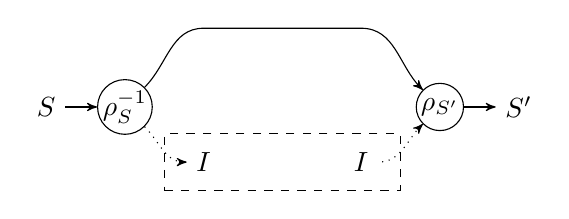
\begin{tikzpicture}
\begin{scope}[on grid]
\node[vert] (l) at (0, 0) {$\rho_S^{-1}$};
\node[vert] (r) at (4, 0) {$\rho_{S'}$};

\node (S) [left of=l] {$S$};
\node (A) [below right = 0.7 and 1 of l] {$I$};
\node (S') [right of=r] {$S'$};
\node (A') [below left = 0.7 and 1 of r] {$I$};

\draw[->] (S) -- (l);
\draw[->, dotted] (l) to[out=south east,in=west] (A);

\draw[<-] (S') -- (r);
\draw[<-, dotted] (r) to[out=south west,in=east] (A');

\draw[->] (l) to[out=north east, in=west] ++(1,1)
 to ++(2,0)
 to[out=east, in=north west] (r)
;

\node[draw,dashed,fit=(A) (A'), inner xsep = 8pt] (box) {};
\end{scope}
\end{tikzpicture}
\end{center}
Or, again omitting the unitors:
\begin{center}
  \begin{tikzpicture}
\begin{scope}[on grid]
\node (S) at (0, 0) {$S$};
\node (S') at (4, 0) {$S$};

\draw[->] (S) -- (S');

\node (I) [below right = 0.7 and 1.4 of S] {$I$};
\node (I') [below left = 0.7 and 1.4 of S'] {$I$};

\node[draw,dashed,fit=(I) (I'), inner xsep = 4pt] (box) {};
\end{scope}
\end{tikzpicture}
\end{center}

\begin{proposition}
  Suppose the monoidal unit $I$ of $\C$ is terminal. Then the set of states $(I, I) \hto (A, A')$ is isomorphic to $\C(I, A)$.
\end{proposition}
\begin{proof}
  First, note that
  \begin{align*}
    \Optic_\otimes((I,I), (A,A'))
    &= \int^{M \in \C} \C(I, M \otimes A) \times \C(M \otimes A', I) \\
    &\cong \int^{M \in \C} \C(I, M \otimes A).
  \end{align*}
  Because the interior of this coend is mute in the contravariant position, the coend is equal to the colimit of the functor $\C(I, - \otimes A) : \C \to \Set$. But $\C$ has a terminal object, so $\int^{M \in \C} \C(I, M \otimes A) \cong \C(I, I \otimes A) \cong \C(I, A)$.
\end{proof}

\begin{proposition}\label{prop:change-of-action-monoidal}
  A monoidal functor $F : \C \to \D$ induces a functor $\Optic(F) : \Optic_\C \to \Optic_\D$.
\end{proposition}
\begin{proof}
  On objects this is simply $\Optic(F)(S, S') = (FS, FS')$. On a morphism $\rep{l}{r} : (S, S') \to (A, A')$, we define
  \begin{align*}
    \Optic(F)(\rep{l}{r}) := \rep{\phi^{-1}_{M,A} (Fl)}{(Fr) \phi_{M,A'}}
  \end{align*}
  where $\phi_{M,A} : FM \otimes FA \to F(M \otimes A)$ is the structure map of the monoidal functor.
  This preserves identities:
  \begin{align*}
  \Optic(F)(\id_{(S, S')}) 
  &= \Optic(F)(\rep{\lambda^{-1}_S}{\lambda_{S'}}) \\
  &= \rep{\phi^{-1}_{I,S} (F\lambda^{-1}_S)}{(F\lambda_{S'}) \phi_{I,S'}} \\
  &= \rep{(\phi^{-1} \otimes S) \phi^{-1}_{I,S} (F\lambda^{-1}_S)}{(F\lambda_{S'}) \phi_{I,S'}(\phi \otimes S) } \\
  &= \rep{(\phi^{-1} \otimes S) \phi^{-1}_{I,S} (F\lambda^{-1}_S)}{(F\lambda_{S'}) \phi_{I,S'}(\phi \otimes S) } \\
  &= \rep{\lambda^{-1}_{FS}}{\lambda_{FS'}} \\
  &= \id_{(FS, FS')}
  \end{align*}
  And given two optics $\rep{l}{r} : (S, S') \hto (A, A')$ and $\rep{l'}{r'} : (R, R') \hto (S, S')$ with residuals $M$ and $M'$, it preserves composition:
\begin{align*}
&\Optic(F)(\rep{l}{r} \circ \rep{l'}{r'})  \\
&= \Optic(F)(\rep{(M' \otimes l)l'}{r'(M' \otimes r)}) \\
&= \rep{\phi^{-1}_{M' \otimes M,A} F((M' \otimes l)l')}{F(r'(M' \otimes r)) \phi_{M' \otimes M,A'}} \\
&= \rep{\phi^{-1}_{M' \otimes M,A} F(M' \otimes l)(Fl')}{(Fr') F(M' \otimes r) \phi_{M' \otimes M,A'}} \\
&= \rep{(\phi^{-1}_{M', M} \otimes A)\phi^{-1}_{M' \otimes M,A} F(M' \otimes l)(Fl')}{(Fr') F(M' \otimes r) \phi_{M' \otimes M,A'}(\phi_{M', M} \otimes A)} \\
&= \rep{(FM' \otimes \phi^{-1}_{M,A})\phi^{-1}_{M',M \otimes A}(F(M' \otimes l)) (Fl')}{(Fr') (F(M' \otimes r)) \phi_{M',M \otimes A'}  (FM' \otimes \phi_{M,A'})} \\
&= \rep{(FM' \otimes \phi^{-1}_{M,A})(FM' \otimes Fl)\phi^{-1}_{M',S} (Fl')}{(Fr') \phi_{M',S'} (FM' \otimes Fr) (FM' \otimes \phi_{M,A'})} \\
&= \rep{(FM' \otimes \phi^{-1}_{M,A} (Fl))(\phi^{-1}_{M',S} (Fl'))}{((Fr') \phi_{M',S'})(FM' \otimes (Fr) \phi_{M,A'})} \\
&= \rep{\phi^{-1}_{M,A} (Fl)}{(Fr) \phi_{M,A'}} \circ \rep{\phi^{-1}_{M',S} (Fl')}{(Fr') \phi_{M',S'}} \\
&= \Optic(F)(\rep{l}{r}) \circ \Optic(F)(\rep{l'}{r'}) 
\end{align*}
The critical move is adding the isomorphism $(\phi_{M', M} \otimes A)$ to both sides of the coend, so that the hexagon axiom for $F$ can be applied.

The structure morphisms for monoidality are given by lifting the structure morphisms for $F$:
\begin{align*}
\phi_{(S, S'), (T, T')} &:= \iota(\phi_{S, T}, \phi_{S', T'}) &&: F(S, S') \otimes F(T, T') \hto F((S, S') \otimes (T, T')) \\
\phi &:= \iota(\phi, \phi) &&: (I, I) \hto F(I, I)
\end{align*}
The axioms follow by lifting the axioms for $F$. More difficult is verifying naturality: \todo{naturality}
\end{proof}

\begin{proposition}\label{prop-optic-functor}
  Collectively this operation defines a 2-functor \[\Optic : \SymmMonCat \to \SymmMonCat.\] \qed
\end{proposition}
\todo{Haven't actually checked natural transformations}
\todo{Also we run into the large coend issue again, it's not defined on every symm mon cat.}

\subsection{Teleological Categories}\label{sec:teleological-categories}
\todo{I think there are strictness issues in this section, but the idea is correct}

In this section we establish a universal property of the $\Optic$ construction. The idea is that every optic $\rep{l}{r} : (S, S') \hto (A, A')$ consists of a morphism $S \to M \otimes A$ and the `formal dual' of a morphism $M \otimes A' \to S'$, composed with a `formal counit' that traces out the object $M$:
\begin{center}
  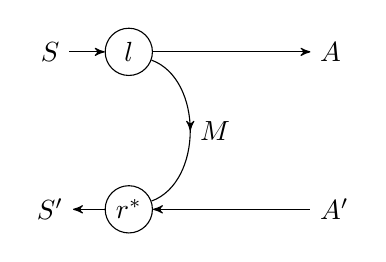
\begin{tikzpicture}
\node[vert] (l) at (0, 0) {$l$};
\node[vert] (r) at (0, -2) {$r^*$};

\node (S) [left of=l]{$S$};
\node (S') [left of=r]{$S'$};

\node (A) [right =2 of l]{$A$};
\node (A') [right = 2 of r]{$A'$};

\draw[->] (S) -- (l);
\draw[->] (l) -- (A);
\draw[<-] (S') -- (r);
\draw[<-] (r) -- (A');

\draw[->-=0.5] (l) to[out = -20, in = 20, edge label=$M$] (r);

%\node (Sin) {$S$};
%\node (f) [vert, right of=Sin] {$f$};
%\node (Sout) [right of=f] {$S$};
%\node (Spout) [right of=Sout] {$S'$};
%\node (g) [vert, right = 0.5 of Spout] {$g$};
%\node (Spin) [right of=g] {$S'$};
%
%\draw[->] (Sin) -- (f);
%\draw[->] (f) -- (Sout);
%\draw[->] (Spout) -- (g);
%\draw[->] (g) -- (Spin);
\end{tikzpicture}
\end{center}

We assume in this section that $\C$ is a \emph{strict} symmetric monoidal category. It will be convenient to equip $\Optic_\otimes$ with a slightly different symmetric monoidal structure. 

\begin{definition}
  The \emph{switched} monoidal product on $\Optic_\otimes$ is given on objects by
  \begin{align*}
    (S, S') \switched (T, T') := (S \otimes T, T' \otimes S')
  \end{align*}
  And on morphisms $\rep{l}{r} : S \hto A$ and $\rep{l'}{r'} : T \hto B$ by:
  \begin{center}
    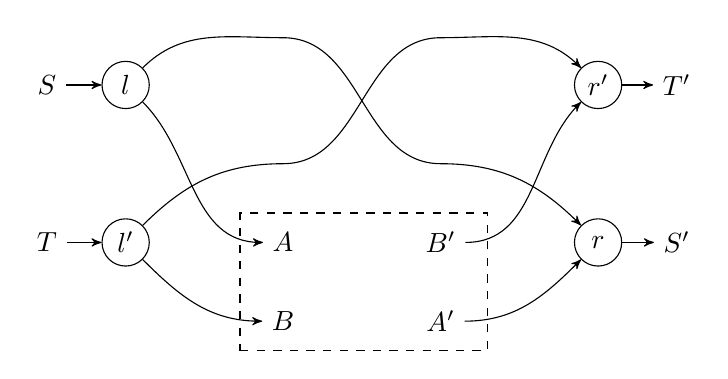
\begin{tikzpicture}
\begin{scope}[on grid]

\node[vert] (l) at (0, 0) {$l$};
\node[vert] (r') at (6, 0) {$r'$};
\node[vert] (l') at (0, -2) {$l'$};
\node[vert] (r) at (6, -2) {$r$};

\node (S) [left of=l] {$S$};
\node (A) [below right = 2 and 2 of l] {$A$};
\node (T') [right of=r'] {$T'$};
\node (B') [below left = 2 and 2 of r'] {$B'$};

\node (T) [left of=l'] {$T$};
\node (B) [below right = 1 and 2 of l'] {$B$};
\node (S') [right of=r] {$S'$};
\node (A') [below left = 1 and 2 of r] {$A'$};

\draw[->] (S) -- (l);
\draw[<-] (T') -- (r');
\draw[->] (T) -- (l');
\draw[<-] (S') -- (r);

\draw[->] (l) to[out=south east,in=west] (A);
\draw[<-] (r') to[out=south west,in=east] (B');
\draw[->] (l') to[out=south east,in=west] (B);
\draw[<-] (r) to[out=south west,in=east] (A');

\draw[->] (l') 
 to[out=north east, in=west] ++(2,1)
 to[out=east, in=west] ++(2,1.6)
 to[out=east, in=north west] (r')
;

\draw[<-] (r) 
 to[out=north west, in=east] ++(-2,1)
 to[out=west, in=east] ++(-2,1.6)
 to[out=west, in=north east] (l)
;


\node[draw,dashed,fit=(A) (A') (B) (B'), inner xsep = 8pt] (box) {};

\end{scope}
\end{tikzpicture}
  \end{center}
\end{definition}

The universal property for $\Optic_\otimes$ given in this section is an argument for this being the ``morally correct'' tensor, although it does seem a little strange. When we later discuss lawful optics, we are forced to use the unswitched tensor to maintain the invariant that our objects are of the form $(X, X)$.

\begin{proposition}
  $(\Optic_\otimes, \switched, (I, I))$ is a symmetric monoidal category that is monoidally equivalent to $\Optic_\otimes$ with the unswitched tensor.
\end{proposition}
\begin{proof}
  The proof that $(\Optic_\otimes, \switched, (I, I))$ is symmetric monoidal is nearly identical to that for the unswitched tensor. Note that due to the switching, the structure morphisms are slightly different:
  \begin{align*}
    \alpha_{(R, R'), (S, S'), (T, T')} &:= \iota(\alpha_{R,S,T}, \alpha_{T',S',R'}^{-1}) \\
    \lambda_{(S, S')} &:= \iota(\lambda_{S}, \rho_{S'}^{-1}) \\
    \rho_{(S, S')} &:= \iota(\rho_{S}, \lambda_{S'}^{-1}) \\
    s_{(S, S'), (T, T')} &:= \iota(s_{S, T}, s_{S', T'})
  \end{align*}

  The categories are monoidally equivalent via the identity functor \[\id : (\Optic_\otimes, \switched, (I, I)) \to (\Optic_\otimes, \otimes, (I, I)),\] where the structure isomorphisms making this functor monoidal are given by
  \begin{align*}
    \iota(\id_{S \otimes S'}, s_{T, T'}) : \id(S, S') \otimes \id(T, T') \to \id((S, S') \switched (T, T'))
  \end{align*}

\end{proof}

\begin{remark}
  Just as in the unswitched case, if $\C$ is a strict monoidal category than so is $(\Optic_\otimes, \switched, (I, I))$.
\end{remark}

\begin{definition}[Compare {\cite[Definition 5.1]{CoherenceForLenses}}]
  A \emph{teleological category is} a symmetric monoidal category $(\C, \otimes, I)$, equipped with:
  \begin{itemize}
  \item A symmetric monoidal subcategory $\C_d$ of \emph{dualisable morphisms} containing all the objects of $\C$, with an involutive symmetric monoidal functor ${(-)}^* : \C_d \to \overline{\C_d^\op}$, where---not finding a standard symbol for such a thing---we mean $\overline{\C_d^\op}$ to be the category with both the direction of the arrows \emph{and} the order of the tensor flipped: ${(A \otimes B)}^* \cong B^* \otimes A^*$. Note that there is therefore a canonical isomorphism $\phi : I \cong I^*$
  \item A symmetric monoidal extranatural family of morphisms $\varepsilon_X : X \otimes X^* \to I$, called \emph{counits}, natural with respect to the morphisms in $\C_d$.
  \end{itemize}
\end{definition}
Unpacking the definition, $\varepsilon$ being a symmetric monoidal extranatural transformation amounts to the following diagrams in $\C$ commuting:
\[
  \begin{tikzcd}
    X \otimes Y^* \ar[r, "f \otimes Y^*"]  \ar[d, "X \otimes f^*", swap] & Y \otimes Y^* \ar[d, "\varepsilon_Y"] \\
    X \otimes X^* \ar[r, "\varepsilon_X", swap] & I
  \end{tikzcd} \hspace{1cm}
  \begin{tikzcd}
    X^* \otimes X \ar[r, "\sigma"]  \ar[dr, "\varepsilon_{X^*}", swap] & X \otimes X^* \ar[d, "\varepsilon_X"] \\
    & I
  \end{tikzcd}\]
\[
  \begin{tikzcd}[column sep = large]
    X \otimes Y \otimes Y^* \otimes X^* \ar[r, "X \otimes \varepsilon_Y \otimes X^*"]  \ar[dr, "\varepsilon_{X \otimes Y}", swap] & X \otimes X^* \ar[d, "\varepsilon_X"] \\
    & I
  \end{tikzcd} \hspace{1cm}
  \begin{tikzcd}
    I \otimes I^* \ar[r,"I \otimes \phi"] \ar[dr, swap, "\varepsilon_I"] & I \ar[d, equal] \\
    & I
  \end{tikzcd}
\]
where $f : X \to Y$ is in $\C_d$.

%%%% The following is a version with duality given by reflection.
% \begin{definition}[{\cite[Definition 5.1]{CoherenceForLenses}}]
%   A \emph{teleological category is} a symmetric monoidal category $(\C, \otimes, I)$, equipped with:
%   \begin{itemize}
%   \item A wide symmetric monoidal subcategory $\C_d$ of \emph{dualisable morphisms}, with an involutive strong symmetric monoidal functor $(-)^* : \C_d \to \C_d^\op$; and,
%   \item A family of morphisms $\varepsilon_X : X \otimes X^* \to I$, called \emph{counits}, natural with respect to the morphisms in $\C_d$, such that
%     \[
%       \begin{tikzcd}
%         X \otimes Y^* \ar[r, "f \otimes Y^*"]  \ar[d, "X \otimes f^*", swap] & Y \otimes Y^* \ar[d, "\varepsilon_Y"] \\
%         X \otimes X^* \ar[r, "\varepsilon_X", swap] & I
%       \end{tikzcd} \hspace{1cm}
%       \begin{tikzcd}
%         X^* \otimes X \ar[r, "s_{X^*, X}"]  \ar[dr, "\varepsilon_{X^*}", swap] & X \otimes X^* \ar[d, "\varepsilon_X"] \\
%         & I
%       \end{tikzcd}
%     \]
%     \[
%       \begin{tikzcd}
%         X \otimes Y \otimes X^* \otimes Y^* \ar[r, "X \otimes s_{Y,X^*} \otimes X^*"]  \ar[dr, "\varepsilon_{X \otimes Y}", swap] & X \otimes X^* \otimes Y \otimes Y^* \ar[d, "\varepsilon_X \otimes \varepsilon_Y"] \\
%         & I
%       \end{tikzcd}
%     \]
%     commute for all $f : X \to Y$ is in $\C_d$.
%   \end{itemize}
% \end{definition}

% \begin{remark}
%   Compact closed categories very nearly form examples of teleological categories. In a compact closed category, there are canonical isomorphisms $(X \otimes Y)^* \cong Y^* \otimes X^*$. In a teleological category, however, duality does not reverse the order of the tensor. \todo{If $\C$ is strict, as it is here, does this matter?}
% \end{remark}

Note that because $\C_d$ is symmetric monoidal and has the same collection of objects as $\C$, the symmetric monoidal structure morphisms of $\C$ must be contained in $\C_d$ and so are dualisable.

\begin{example}
  Any symmetric monoidal category with terminal monoidal unit is trivially teleological, setting the dualisable morphisms to be the structure maps of the monoidal category.
\end{example}

\begin{example}
  Any compact closed category is a teleological category, where every morphism is dualisable and the unit morphisms have been forgotten.
\end{example}

\begin{remark}
This definition of teleological category differs from the original one, in that the duality switches the order of the tensor product. We do this so that compact closed category are teleological, but the bookkeeping becomes more confusing.
\end{remark}

%\begin{example}
%  \todo{The funny graph example from the coherence paper?}
%\end{example}

%There are few surprises in the following definitions.

\begin{definition}
  A \emph{teleological functor} $F : \C \to \D$ is a symmetric monoidal functor that restricts to a functor $F_d : \C_d \to \D_d$ on the dualisable subcategories, commutes \todo{strictly?} with the duality and such that the counits are preserved:
  \[
   \begin{tikzcd}
    F(X \otimes X^*) \ar[r, "\phi_{X, X^*}"]  \ar[d, "F\varepsilon_X", swap] & FX \otimes FX^* \ar[d, "\varepsilon_{FX}"] \\
    FI \ar[r, "\phi", swap] & I
  \end{tikzcd}
  \]
\end{definition} 

%\begin{definition}
%  A \emph{teleological natural transformation} $\alpha : F \Rightarrow G$ is a monoidal natural transformation that is additionally compatible with the dualisation:
%  \[
%  \begin{tikzcd}
%    (FX)^* \ar[r, "\cong"]  \ar[d, "(\alpha_X)^*", swap] & F(X^*) \ar[d, "\alpha_{X^*}"] \\
%    (GX)^* \ar[r, "\cong", swap] & G(X^*)
%  \end{tikzcd}
%  \]
%  whenever $\alpha_X$ is dualisable. \todo{Does adding this condition make sense?}
%\end{definition}

Together we have $\Tele$, the subcategory of $\SymmMonCat$ given by teleological categories and teleological functors. There are evident functors $U : \Tele \to \SymmMonCat$ and ${(-)}_d : \Tele \to \SymmMonCat$, that take a teleological category to its underlying symmetric monoidal category and subcategory of dualisable morphisms respectively.

The definition of teleological category suggests a string diagram calculus similar to that for compact closed categories, but where only counits exist, and only morphisms known to be dualisable may be passed around a counit by extranaturality. We have of course not proven that such a calculus is sound for teleological categories, but we trust that a sceptical reader could verify our arguments equationally.

\begin{proposition}
  $\Optic_\otimes$ forms a teleological category, where:
  \begin{itemize}
  \item The dualisable morphisms are all morphisms of the form $\iota(f, g)$;
  \item The involution is given on objects by ${(S, S')}^* := (S', S)$, and on morphisms by \[\iota{(f, g)}^* := \iota(g, f);\]
  \item The counit $\varepsilon_{(S, S')} : (S, S') \switched {(S, S')}^* = (S \otimes S', S \otimes S') \to (I, I)$ is given by the connector: \[\varepsilon_{(S, S')} := c_{S \otimes S'}.\]
  \end{itemize}
\end{proposition}
\begin{proof}
  That morphisms of the form $\iota(f, g)$ constitute a category is clear. The functor ${(-)}^*$ is a symmetric monoidal involution, in fact it is strictly so:
  \begin{align*}
    \left( (S, S') \switched (T, T') \right)^*
    &= \left( S \otimes T, T' \otimes S' \right)^* \\
    &= \left(T' \otimes S', S \otimes T  \right) \\
    &= (T', T) \switched (S', S) \\
    &= (T, T')^* \switched (S, S')^*
  \end{align*}

  To check extranaturality of $\varepsilon$, suppose we have a dualisable optic $\iota(f, g) : (S, S') \hto (T, T')$, so $f : S \to T$ and $g : T' \to S'$. Luckily here all the switching in the definitions cancel out! Extranaturality is witnessed by the equality of the string diagrams:
  \begin{center}
    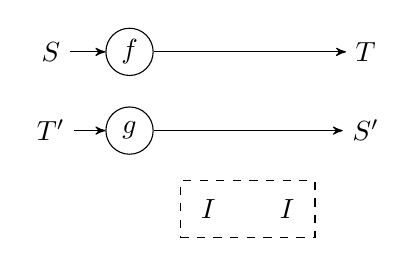
\begin{tikzpicture}
\begin{scope}[on grid]
\node (S) at (0, 0) {$S$};
\node (S') at (4, 0) {$T$};
\node (T) [below = 1 of S] {$T'$};
\node (T') [below = 1 of S'] {$S'$};
\node[vert] (f) [right = 1 of S] {$f$};
\node[vert] (g) [right = 1 of T] {$g$};

\draw[->] (S) -- (f);
\draw[->] (f) -- (S');

\draw[->] (T) -- (g);
\draw[->] (g) -- (T');

\node (I) [below right = 1 and 2 of T] {$I$};
\node (I') [below left = 1 and 1 of T'] {$I$};

\node[draw,dashed,fit=(I) (I'), inner xsep = 4pt] (box) {};
\end{scope}
\end{tikzpicture}
    \qquad \raisebox{1.5cm}{$=$} \qquad
    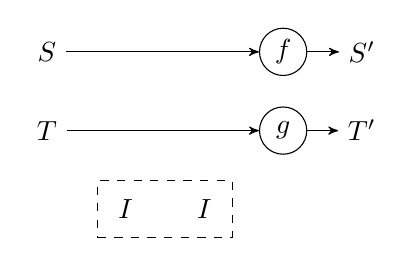
\begin{tikzpicture}
\begin{scope}[on grid]
\node (S) at (0, 0) {$S$};
\node (S') at (4, 0) {$S'$};
\node (T) [below = 1 of S] {$T$};
\node (T') [below = 1 of S'] {$T'$};
\node[vert] (f) [left = 1 of S'] {$f$};
\node[vert] (g) [left = 1 of T'] {$g$};

\draw[->] (S) -- (f);
\draw[->] (f) -- (S');

\draw[->] (T) -- (g);
\draw[->] (g) -- (T');

\node (I) [below right = 1 and 1 of T] {$I$};
\node (I') [below left = 1 and 2 of T'] {$I$};

\node[draw,dashed,fit=(I) (I'), inner xsep = 4pt] (box) {};
\end{scope}
\end{tikzpicture}
  \end{center}
  For symmetry:
  \begin{center}
    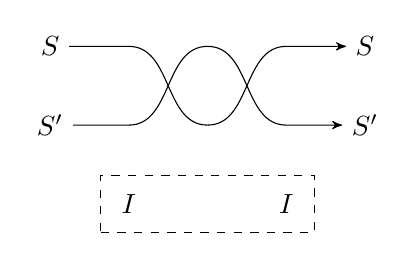
\begin{tikzpicture}
\begin{scope}[on grid]
\node (S) at (0, 0) {$S$};
\node (S2) at (4, 0) {$S$};
\node (S') [below = 1 of S] {$S'$};
\node (S'2) [below = 1 of S2] {$S'$};

\draw[->] (S) -- ++(1,0) to[out = east, in = west] ++(1,-1) to[out = east, in = west] ++ (1,1) -- (S2);
\draw[->] (S') -- ++(1,0) to[out = east, in = west] ++(1,1) to[out = east, in = west] ++ (1,-1) -- (S'2);

\node (I) [below right = 1 and 1 of S'] {$I$};
\node (I') [below left = 1 and 1 of S'2] {$I$};

\node[draw,dashed,fit=(I) (I'), inner xsep = 4pt] (box) {};
\end{scope}
\end{tikzpicture}
    \qquad \raisebox{1.5cm}{$=$} \qquad
    \begin{tikzpicture}
\begin{scope}[on grid]
\node (S) at (0, 0) {$S$};
\node (S2) at (4, 0) {$S$};
\node (S') [below = 1 of S] {$S'$};
\node (S'2) [below = 1 of S2] {$S'$};

\draw[->] (S) -- (S2);
\draw[->] (S') -- (S'2);

\node (I) [below right = 1 and 1 of S'] {$I$};
\node (I') [below left = 1 and 1 of S'2] {$I$};

\node[draw,dashed,fit=(I) (I'), inner xsep = 4pt] (box) {};
\end{scope}
\end{tikzpicture}
  \end{center}
  And for monoidality there is essentially nothing to do in the graphical calculus. 
  \begin{center}
    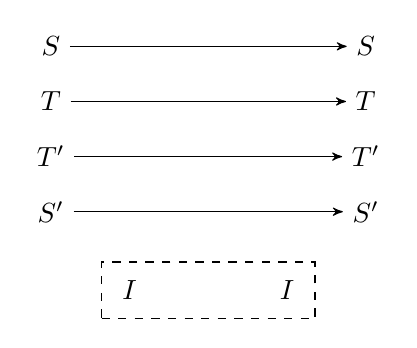
\begin{tikzpicture}
\begin{scope}[on grid]
\node (S) at (0, 0) {$S$};
\node (S2) at (4, 0) {$S$};
\node (T) [below = 0.7 of S] {$T$};
\node (T2) [below = 0.7 of S2] {$T$};
\node (T') [below = 0.7 of T] {$T'$};
\node (T'2) [below = 0.7 of T2] {$T'$};
\node (S') [below = 0.7 of T'] {$S'$};
\node (S'2) [below = 0.7 of T'2] {$S'$};

\draw[->] (S) -- (S2);
\draw[->] (T) -- (T2);
\draw[->] (S') -- (S'2);
\draw[->] (T') -- (T'2);

\node (I) [below right = 1 and 1 of S'] {$I$};
\node (I') [below left = 1 and 1 of S'2] {$I$};

\node[draw,dashed,fit=(I) (I'), inner xsep = 4pt] (box) {};
\end{scope}
\end{tikzpicture}
    \qquad \raisebox{2cm}{$=$} \qquad
    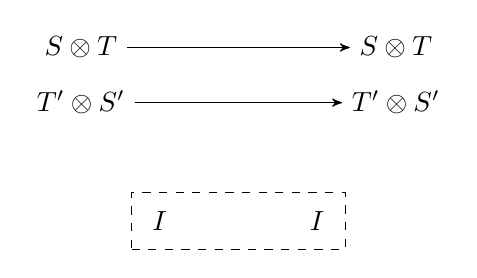
\begin{tikzpicture}
\begin{scope}[on grid]
\node (S) at (0, 0) {$S \otimes T$};
\node (S2) at (4, 0) {$S \otimes T$};
\node (T) [below = 0.7 of S] {$T' \otimes S'$};
\node (T2) [below = 0.7 of S2] {$T' \otimes S'$};

\draw[->] (S) -- (S2);
\draw[->] (T) -- (T2);

\node (I) [below right = 1.5 and 1 of T] {$I$};
\node (I') [below left = 1.5 and 1 of T2] {$I$};

\node[draw,dashed,fit=(I) (I'), inner xsep = 4pt] (box) {};
\end{scope}
\end{tikzpicture}
  \end{center}

  Note that the diagrams that are required to commute in the definition of teleological category all terminate with the unit $I$, so in view of Proposition~\ref{prop-costates} we should not be surprised that they correspond to equality of maps in $\C$.
\end{proof}

      %       \todo{They stress about the empty set, have I avoided that issue?}

\begin{proposition}
  The functor $\Optic : \SymmMonCat \to \SymmMonCat$ of Proposition~\ref{prop-optic-functor} has its image in the subcategory $\Tele$.
\end{proposition}
\begin{proof}
  We must show that for a symmetric monoidal functor $F : \C \to \D$, the induced functor $F : \Optic_\C \to \Optic_\D$ is teleological.

  First, $F$ preserves the dualisable morphisms. If $\iota(f, g) : (S, S') \hto (A, A')$,
  \begin{align*}
    F\iota(f, g)
    &= F(\rep{\lambda_A^{-1} f}{g \lambda_{A'}}) \\
    &= \rep{\phi^{-1}_{I,A} (F(\lambda_A^{-1} f))}{(F(g \lambda_{A'})) \phi_{I,A'}} \\
    &= \rep{\phi^{-1}_{I,A} (F\lambda_A^{-1}) (Ff)}{(Fg)(F \lambda_{A'}) \phi_{I,A'}} \\
    &= \rep{(\phi^{-1}_I \otimes FA) \phi^{-1}_{I,A} (F\lambda_A^{-1}) (Ff)}{(Fg)(F \lambda_{A'}) \phi_{I,A'} (\phi_I \otimes FA)} \\
    &= \rep{\lambda_{FA}^{-1} (Ff)}{(Fg)\lambda_{FA'}} \\
    &= \iota(Ff, Fg)
  \end{align*}

  And it also preserves the counits:
  \begin{align*}
    F(\varepsilon_{(S, S')})
    &= F(c_{S \otimes S'}) \\
    &= F(\rep{\rho_S^{-1}}{\rho_{S'}}) \\
    &= \rep{\phi^{-1}_{S,I} (F \rho_S^{-1})}{(F \rho_{S'}) \phi_{S',I}} \\
    &= \rep{(FS \otimes \phi_I^{-1}) \phi^{-1}_{S,I} (F \rho_S^{-1})}{(F \rho_{S'}) \phi_{S',I} (FS \otimes \phi_I)} \\
    &= \rep{\rho_{FS}^{-1}}{\rho_{FS'}} \\
    &= \varepsilon_{(FS, FS')}
  \end{align*}

%  \todo{This works fine when $\C$ is not strict}
\end{proof}

      %       \begin{proposition}
      %       Suppose $\langle l, r \rangle : (S, S') \hto (A, A')$ has residual $M$. Then
      %       \begin{align*}
      %       \langle l, r \rangle = (\varepsilon_{(M, I)} \otimes (A, A'))\iota(l, r).
      %     \end{align*}
      %       \end{proposition}
      %       \begin{proof}
      %       First note that because $\C$ is strict monoidal, the counit $\varepsilon_{(M, I)} : (M \otimes I, M \otimes I) = (M, M) \hto (I, I)$ is equal to the connector $c_M : (M, M) \hto (I, I)$.
      %
      %       The claim then holds, as any optic
      %       \begin{center}
      %       \begin{tikzpicture}
\node[vert] (l) at (0, 0) {$l$};
\node[vert] (r) at (4, 0) {$r$};

\node (S) [left of=l] {$S$};
\node (A) [below right = 0.7 and 1 of l] {$A$};
\node (S') [right of=r] {$S'$};
\node (A') [below left = 0.7 and 1 of r] {$A'$};

\draw[->] (S) -- (l);
\draw[->] (l) to[out=south east,in=west] (A);

\draw[<-] (S') -- (r);
\draw[<-] (r) to[out=south west,in=east] (A');

\draw[->] (l) to[rrel, out=north east, in=west] (1,1)
 to +(2,0)
 to[out=east, in=north west] (r)
;

\node[draw,dashed,fit=(A) (A'), inner xsep = 8pt] (box) {};
\end{tikzpicture}
      %       \end{center}
      %       is equal to the composite
      %       \begin{center}
      %       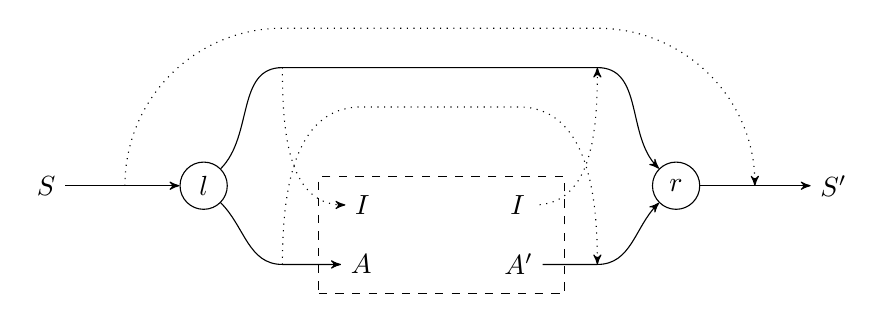
\begin{tikzpicture}
\begin{scope}[on grid]

\node[vert] (l) at (0, 0) {$l$};
\node[vert] (r) at (6, 0) {$r$};

\node (S) [left= 2 of l] {$S$};
\node (A) [below right = 1 and 2 of l] {$A$};
\node (S') [right= 2 of r] {$S'$};
\node (A') [below left = 1 and 2 of r] {$A'$};

\draw[->] (S) -- (l);
\draw[->] (l) 
  to[out=south east,in=west] ($(l) + (1, -1)$)
  to[out=east, in=west] (A);

\draw[<-] (S') -- (r);
\draw[<-] (r) 
  to[out=south west,in=east] ($(r) + (-1, -1)$)
  to[out=west, in=east] (A');

\draw[->] (l) to[out=north east, in=west] ++(1,1.5) coordinate (Mleft) 
 to  ($(r) + (-1, 1.5)$) coordinate (Mright)
 to[out=east, in=north west] (r)
;

\node (I) [below right = 1.5 and 0.8 of Mleft] {$I$};
\node (I') [below left = 1.5 and 0.8 of Mright] {$I$};

\draw[->, dotted] (Mleft) 
  to[out=south, in=west] (I);
\draw[<-, dotted] (Mright) 
  to[out=south, in=east] (I');

\draw[->, dotted]  ($(l) + (-1, 0)$)
 to[out=north, in=west] ++(2,2)
 to[out=east, in=west] ($(r) + (-1, 2)$)
 to[out=east, in=north] ($(r) + (1, 0)$)
;

\draw[->, dotted]  ($(A) + (-1, 0)$)
 to[out=north, in=west] ++(1,2)
 to[out=east, in=west] ($(A') + (0, 2)$)
 to[out=east, in=north] ($(A') + (1, 0)$)
;

%
%\node[vert] (l') at (0, -2) {$l'$};
%\node[vert] (r') at (6, -2) {$r'$};
%
%\node (T) [left of=l'] {$T$};
%\node (B) [below right = 1 and 2 of l'] {$B$};
%\node (T') [right of=r'] {$T'$};
%\node (B') [below left = 1 and 2 of r'] {$B'$};
%
%\draw[->] (T) -- (l');
%\draw[->] (l') to[out=south east,in=west] (B);
%
%\draw[<-] (T') -- (r');
%\draw[<-] (r') to[out=south west,in=east] (B');
%
%\draw[->] (l') 
% to[rrel, out=north east, in=west] (2,2)
% to ++(2,0)
% to[out=east, in=north west] (r')
%;
%

\node[draw,dashed,fit=(A) (A') (I) (I'), inner xsep = 8pt] (box) {};

\end{scope}
\end{tikzpicture}
      %       \end{center}
      %       where we have drawn the normally invisible strings corresponding to the unit $I$.
      %       \end{proof}

Our goal now is to establish the universal property of $\Optic_\otimes$. The following proposition gives that an optic decomposes in a canonical way:

\begin{proposition}\label{prop-optic-decompose}
  Suppose $\rep{l}{r} : (S, S') \hto (A, A')$ has residual $M$. Then
  \begin{align*}
    \rep{l}{r} = ((A, I) \switched \varepsilon_{(M, I)} \switched (I, A'))(j(s_{M,A}l) \switched j(rs_{A',M})^*)
  \end{align*}
  where $j : \C \to \Optic_\otimes$ is the functor $j(A) := \iota(A, I)$.
\end{proposition}
The symmetries in the above expression could have been avoided if $\Optic$ had been defined as $\int^{M \in \C} \C(S, A \otimes M) \times \C(A' \otimes M, S')$, but it is too late to change the convention now!
\begin{proof}
  First note that because $\C$ is strict monoidal, the counit $\varepsilon_{(M, I)} : (M \otimes I, M \otimes I) = (M, M) \hto (I, I)$ is equal to the connector $c_M : (M, M) \hto (I, I)$.

  Then, up to strictness of the monoidal unit, we are composing the two optics
  \begin{center}
    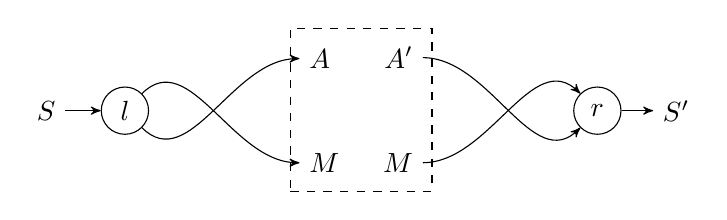
\begin{tikzpicture}

\node (l) [vert] at (0, 0) {$l$};
\node (S) [left of=l] {$S$};
\node (A) [above right = 0.2 and 2 of l] {$A$};
\node (M) [below right = 0.2 and 2 of l] {$M$};

\node (r) [vert] at (6, 0) {$r$};
\node (S') [right of=r] {$S'$};
\node (A') [above left = 0.2 and 2 of r] {$A'$};
\node (M') [below left = 0.2 and 2 of r] {$M$};

\draw[->] (S) -- (l);
\draw[->] (r) -- (S');

\draw[->] (l) to[out=south east, in=west] (A);
\draw[->] (l) to[out=north east, in=west] (M);

\draw[<-] (r) to[out=south west, in=east] (A');
\draw[<-] (r) to[out=north west, in=east] (M');

\node[draw,dashed,fit=(A) (A') (M) (M')] (box) {};
\end{tikzpicture}
  \end{center}
  and
  \begin{center}
    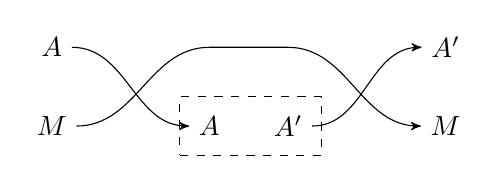
\begin{tikzpicture}
\begin{scope}[on grid]

\node (A) at (0, 0) {$A$};
\node (M) [below = 1 of A] {$M$};
\node (A') at (5, 0) {$A'$};
\node (M') [below = 1 of A'] {$M$};

\node (Aout) [below right = 1 and 2 of A] {$A$};
\node (A'out) [below left= 1 and 2 of A'] {$A'$};

\draw[->] (A) to[out=east, in=west] (Aout);
\draw[<-] (A') to[out=west, in=east] (A'out);

\draw[->] (M) to[out=east, in=west] ($(Aout) + (0,1)$)
to[out=east, in=west] ($(A'out) + (0,1)$)
to[out=east, in=west] (M');

\node[draw,dashed,fit=(Aout) (A'out) ] (box) {};

\end{scope}
\end{tikzpicture}
  \end{center}
  so the two pairs of twists cancel, and we are left exactly with the diagram for $\rep{l}{r}$.
\end{proof}

\begin{theorem}
  \label{optic-is-free-teleological-cat}
  Suppose $\C$ is a strict symmetric monoidal category and $\T$ is a teleological category. For all symmetric monoidal functors $F : \C \to \T_d$, there exists a teleological functor $K : \Optic_\otimes \to \T$, unique up to teleological natural isomorphism with the property $Kj \cong F$.
\end{theorem}
\begin{proof}
  We begin by constructing $K$. Note that any $(S, S')$ in $\Optic_\otimes$ can be written as $j(S) \switched j(S')^*$, so on objects define $K(S, S') = FS \otimes (FS')^*$. Suppose $\rep{l}{r} : (S, S') \hto (A, A')$ is an optic. By the previous Proposition,
  \begin{align*}
    \rep{l}{r} = ((A, I) \switched \varepsilon_{(M, I)} \switched (I, A'))(j(s_{M,A}l) \switched j(rs_{A', M})^*)
  \end{align*}
  So up to isomorphism we are forced to define
  \begin{align*}
    K\rep{l}{r} = (FA \otimes \varepsilon_{FM} \otimes (FA')^*)(F(s_{M,A}l) \otimes (F(rs_{A', M}))^* )
  \end{align*}
  The diagram for $K\rep{l}{r}$ in $\T$ is as follows:
  \begin{center}
    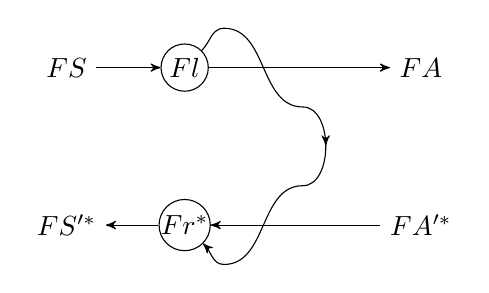
\begin{tikzpicture}
\begin{scope}[on grid]

\node[vert] (l) at (0, 0) {$Fl$};
\node[vert] (r) at (0, -2) {$Fr^*$};

\node (S) [left = 1.5 of l]{$FS$};
\node (S') [left = 1.5 of r]{$FS'^*$};

\node (A) [right =3 of l]{$FA$};
\node (A') [right = 3 of r]{$FA'^*$};

\draw[->] (S) -- (l);
\draw[->] (l) -- (A);
\draw[<-] (S') -- (r);
\draw[<-] (r) -- (A');

\draw[->-=0.5, ->] (l) 
to[out=north east, in=west] ($(l) + (0.5,0.5)$)
to[out=east, in=west] ($(l) + (1.5,-0.5)$)
to[out=east, in=east] ($(r) + (1.5,0.5)$)
to[out=west, in=east] ($(r) + (0.5,-0.5)$)
to[out=west, in=south east] (r);
\end{scope}
\end{tikzpicture}
  \end{center}
  
%  \begin{align*}
%    K\rep{(f \otimes A) l}{r}
%    &= (FA \otimes \varepsilon_{FM} \otimes (FA')^*)(F(s_{M,A}(f \otimes A)l) \otimes (F(rs_{A',M}))^* ) \\
%    &= (FA \otimes \varepsilon_{FM} \otimes (FA')^*)(F((A \otimes f)s_{N,A}l) \otimes (F(rs_{A',M}))^* ) \\
%    % &= (FA \otimes \varepsilon_{FM} \otimes (FA')^*)(FA \otimes Ff \otimes FM \otimes FA')(F(s_{N,A}l) \otimes (F(rs_{A',M}))^* ) \\
%    &= (FA \otimes (\varepsilon_{FM} (Ff \otimes FM)) \otimes (FA')^*)(F(s_{N,A}l) \otimes (F(rs_{A',M}))^* ) \\
%    &= (FA \otimes (\varepsilon_{FN} (FN \otimes (Ff)^*)) \otimes (FA')^*)(F(s_{N,A}l) \otimes (F(rs_{A',M}))^* ) \\
%    &= (FA \otimes \varepsilon_{FN} \otimes (FA')^*)(F(s_{N,A}l) \otimes (F(rs_{A',M}(A' \otimes f)))^* ) \\
%    &= (FA \otimes \varepsilon_{FN} \otimes (FA')^*)(F(s_{N,A}l) \otimes (F(r(f \otimes A')s_{A',N}))^* ) \\
%    &= K\rep{ l}{r (f \otimes A')}
%  \end{align*}

There are now a lot of things to check. 
\begin{itemize}
\item Well-definedness: Suppose we have two optics related by the coend relation:
  \begin{align*}
    \rep{(f \otimes A) l}{r} = \rep{l}{r (f \otimes A')}
  \end{align*}
  Then well-definedness is shown by the equivalence of diagrams
  \begin{center}
    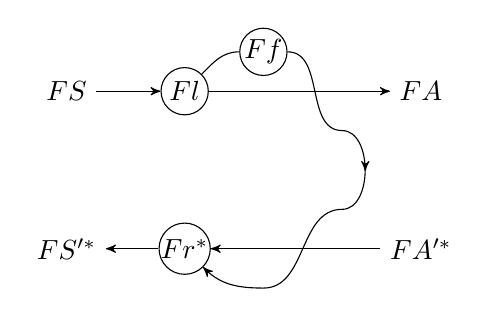
\begin{tikzpicture}
\begin{scope}[on grid]

\node[vert] (l) at (0, 0) {$Fl$};
\node[vert] (r) at (0, -2) {$Fr^*$};
\node[vert] (f) at (1, 0.5) {$Ff$};

\node (S) [left = 1.5 of l]{$FS$};
\node (S') [left = 1.5 of r]{$FS'^*$};

\node (A) [right =3 of l]{$FA$};
\node (A') [right = 3 of r]{$FA'^*$};


\draw[->] (S) -- (l);
\draw[->] (l) -- (A);
\draw[<-] (S') -- (r);
\draw[<-] (r) -- (A');

\draw (l) 
to[out=north east, in=west] (f);

\draw[->-=0.4, ->] (f) 
to[out=east, in=west] ($(f) + (1,-1)$)
to[out=east, in=east] ($(r) + (2,0.5)$)
to[out=west, in=east] ($(r) + (1,-0.5)$)
to[out=west, in=south east] (r);
\end{scope}
\end{tikzpicture}
    \qquad \raisebox{1.5cm}{$=$} \qquad
    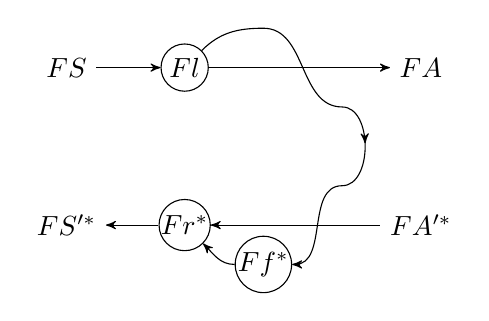
\begin{tikzpicture}
\begin{scope}[on grid]

\node[vert] (l) at (0, 0) {$Fl$};
\node[vert] (r) at (0, -2) {$Fr^*$};
\node[vert] (fd) at (1, -2.5) {$Ff^*$};

\node (S) [left = 1.5 of l]{$FS$};
\node (S') [left = 1.5 of r]{$FS'^*$};

\node (A) [right =3 of l]{$FA$};
\node (A') [right = 3 of r]{$FA'^*$};


\draw[->] (S) -- (l);
\draw[->] (l) -- (A);
\draw[<-] (S') -- (r);
\draw[<-] (r) -- (A');

\draw[->, ->-=0.6] (l) 
to[out=north east, in=west] ($(l) + (1,0.5)$)
to[out=east, in=west] ($(l) + (2,-0.5)$)
to[out=east, in=east] ($(fd) + (1,1)$)
to[out=west, in=east] (fd);
\draw[->] (fd)
to[out=west, in=south east] (r);
\end{scope}
\end{tikzpicture}
  \end{center}
  using naturality of the symmetry and extranaturality of the counit.
\item Functoriality: We have an equivalence of diagrams
  \begin{center}
    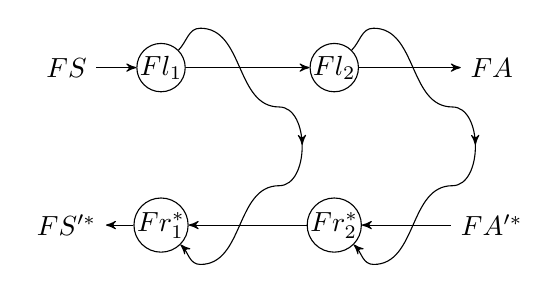
\begin{tikzpicture}
\begin{scope}[on grid]

\node[vert] (l) at (0, 0) {$Fl_1$};
\node[vert] (r) at (0, -2) {$Fr_1^*$};

\node (S) [left = 1.2 of l]{$FS$};
\node (S') [left = 1.2 of r]{$FS'^*$};

\node[vert] (l') [right = 2.2 of l] {$Fl_2$};
\node[vert] (r') [right = 2.2 of r] {$Fr_2^*$};

\node (A) [right = 2 of l']{$FA$};
\node (A') [right = 2 of r']{$FA'^*$};

\draw[->] (S) -- (l);
\draw[->] (l) -- (l');
\draw[->] (l') -- (A);
\draw[<-] (S') -- (r);
\draw[<-] (r) -- (r');
\draw[<-] (r') -- (A');

\draw[->-=0.5, ->] (l) 
to[out=north east, in=west] ($(l) + (0.5,0.5)$)
to[out=east, in=west] ($(l) + (1.5,-0.5)$)
to[out=east, in=east] ($(r) + (1.5,0.5)$)
to[out=west, in=east] ($(r) + (0.5,-0.5)$)
to[out=west, in=south east] (r);

\draw[->-=0.5, ->] (l') 
to[out=north east, in=west] ($(l') + (0.5,0.5)$)
to[out=east, in=west] ($(l') + (1.5,-0.5)$)
to[out=east, in=east] ($(r') + (1.5,0.5)$)
to[out=west, in=east] ($(r') + (0.5,-0.5)$)
to[out=west, in=south east] (r');
\end{scope}
\end{tikzpicture}
    \quad \raisebox{1.5cm}{$=$} \quad
    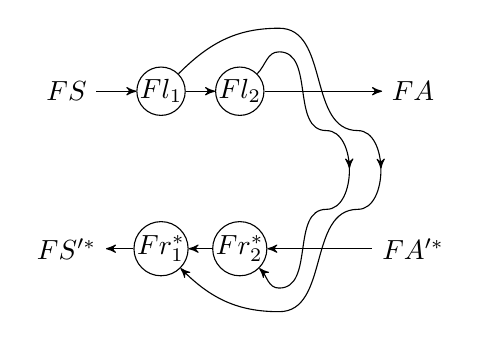
\begin{tikzpicture}
\begin{scope}[on grid]

\node[vert] (l) at (0, 0) {$Fl_1$};
\node[vert] (r) at (0, -2) {$Fr_1^*$};

\node (S) [left = 1.2 of l]{$FS$};
\node (S') [left = 1.2 of r]{$FS'^*$};

\node[vert] (l') [right = 1 of l] {$Fl_2$};
\node[vert] (r') [right = 1 of r] {$Fr_2^*$};

\node (A) [right = 2.2 of l']{$FA$};
\node (A') [right = 2.2 of r']{$FA'^*$};

\draw[->] (S) -- (l);
\draw[->] (l) -- (l');
\draw[->] (l') -- (A);
\draw[<-] (S') -- (r);
\draw[<-] (r) -- (r');
\draw[<-] (r') -- (A');

\draw[->-=0.5, ->] (l) 
to[out=north east, in=west] ($(l) + (1.5,0.8)$)
to[out=east, in=west] ($(l) + (2.5,-0.5)$)
to[out=east, in=east] ($(r) + (2.5,0.5)$)
to[out=west, in=east] ($(r) + (1.5,-0.8)$)
to[out=west, in=south east] (r);

\draw[->-=0.5, ->] (l') 
to[out=north east, in=west] ($(l') + (0.5,0.5)$)
to[out=east, in=west] ($(l') + (1.1,-0.5)$)
to[out=east, in=east] ($(r') + (1.1,0.5)$)
to[out=west, in=east] ($(r') + (0.5,-0.5)$)
to[out=west, in=south east] (r');
\end{scope}
\end{tikzpicture}
  \end{center}
using naturality of the symmetry and monoidality of the counit.
\item Preservation of duals:
\begin{align*}
K((S, S')^*) 
= K(S', S) 
= FS' \otimes (FS)^*
\cong (FS \otimes (FS')^*)^*
= (K(S, S'))^*
\end{align*}
\item Monoidality: We have the isomorphism \[ \phi_{(S, S'),(T, T')} : K((S, S') \switched (T, T')) \to K(S, S') \otimes K(T, T')\] given by the composite
\begin{align*}
K((S, S') \switched (T, T')) 
&= K(S \otimes T, T' \otimes S) \\
&= F(S \otimes T) \otimes F(T' \otimes S')^* \\
&\xrightarrow{\phi_{S, T} \otimes \phi_{T', S'}^*} FS \otimes FT \otimes (FS')^* \otimes (FT')^* \\
&\xrightarrow{FS \otimes s \otimes (FT')^*} FS \otimes (FS')^* \otimes FT \otimes (FT')^* \\
&= K(S, S') \otimes K(T, T')
\end{align*}
using the symmetry of $\T$, and
\begin{align*}
K(I, I) 
&= FI \otimes (FI)^* \\
&\cong I \otimes I^* \\
&\cong I
\end{align*}
That these obey the required coherences is straightforward. More difficult is showing that the first isomorphism is natural in $(S, S')$ and $(T, T')$: \todo{todo}
\item Preservation of dualisable morphisms:  For a morphism $\iota(f, g)$:
\begin{align*}
K(\iota(f, g))
    &= K(\rep{\lambda_A^{-1} f}{g \lambda_{A'}}) \\
    &= (FA \otimes \varepsilon_{FI} \otimes (FA')^*)(F(s_{I,A}\lambda_A^{-1} f) \otimes (F(g \lambda_{A'}s_{A', I}))^* ) \\
    &= (FA \otimes (FA')^*)(Ff \otimes (Fg)^* ) \\
    &= Ff \otimes (Fg)^*
\end{align*}
and this is dualisable, as dualisability is preserved by taking the monoidal product and duals.
\item Preservation of counits: 
\begin{align*}
K(\varepsilon_{(S, S')}) 
&= K(c_{S \otimes S'}) \\
&= K(\rep{\rho_{S \otimes S'}^{-1}}{\rho_{S \otimes S'}}) \\
&= (FI \otimes \varepsilon_{F(S \otimes S')} \otimes (FI)^*)(F(s_{S \otimes S',I}\rho_{S \otimes S'}^{-1}) \otimes (F(\rho_{S \otimes S'} s_{I, S \otimes S'}))^* ) \\
&= (\varepsilon_{F(S \otimes S')})(F(S \otimes S') \otimes F(S \otimes S')^* ) \\
&= \varepsilon_{F(S \otimes S')}
\end{align*}
by strictness of the monoidal unit. This morphism is indeed equal to the composite $\varepsilon_{K(S, S')} \phi_{(S, S'), (S, S')^*}$, using extranaturality to commute the structure maps $\phi_{S, S'}$ of $F$ and the symmetry of $\T$ through $\varepsilon$. \todo{write details?}
\end{itemize}
\end{proof}

\begin{theorem}
$\Optic : \SymmMonCat \to \Tele$ is left biadjoint to the underlying dualisable morphisms functor ${(-)}_d : \Tele \to \SymmMonCat$
\end{theorem}
\begin{proof}
\todo{figure out exactly what else needs proving}
\end{proof}

\subsection{Optics for a Monoidal Action}

To capture more of the optic variants available in the Haskell \lenslib{} library, we generalise to the case of a monoidal action of one category on another.

\begin{definition}
  Let $\C$ be a category and $(\M, \otimes, I)$ a monoidal category. An \emph{action of $\M$ on $\C$} is a monoidal functor $a : \M \to [\C, \C]$. For two objects $M \in \M$ and $A \in \C$, the action $a(M)(A)$ is abbreviated $MA$. The tensor product in $\M$ will also be written as juxtaposition, so $(NM)A \cong N(MA)$.
\end{definition}

Given such an action, we define
\begin{align*}
  \Optic_\M((S, S'), (A, A')) := \int^{M \in \M} \C(S, MA) \times \C(MA', S')
\end{align*}

The following are analogous to Propositions~\ref{prop-optic-is-cat} and \ref{prop:change-of-action-monoidal}.

\begin{proposition}
  We have a category $\Optic_\M$ and a functor $\iota : \C \times \C^\op \to \Optic_\M$. \qed
\end{proposition}

\begin{definition}
Given two categories equipped with monoidal actions $(\M, \C)$ and $(\N, D)$, a \emph{morphism of actions} is a monoidal functor $F^\bullet : \M \to N$ and a functor $F : \C \to \D$ that commutes with the actions, in the sense that there exist natural isomorphisms
  \begin{align*}
  \phi &: F(I A) \to (F^\bullet I)(FA) \\
  \phi_{M,A} &: F(MA) \to (F^\bullet M)(F A) 
  \end{align*}
satisfying conditions analogous to those for a monoidal functor.
\end{definition}

\begin{proposition}\label{prop:change-of-action}
If $F : (\M, \C) \to (\N, D)$, is a morphism of actions, there is an induced functor $\Optic(F) : \Optic_\M \to \Optic_\N$. \qed
\end{proposition}

For the remainder of the paper we work in this more general setting.

      %       \begin{proposition}
      %       \todo{Entrywise Coproduct}
      %       \end{proposition}
      %
      %       \begin{remark}
      %       The motivating example here is that of coproducts distributing over the tensor product.
      %       \end{remark}

\section{Lawful Optics}\label{sec:lawful-optics}
\todo{intro}

In this section I use $;$ to denote composition of $\C$ in diagrammatic order. The reason for this is that the coend relation can be applied simply by shifting the position of $\mid$ in a representative:
\begin{align*}
\rep{l;\phi A}{r} = \rep{l}{\phi A;r}
\end{align*}

\todo{Should I switch everything else to use diagrammatic order?}

\begin{remark}
  In this section we will focus only on optics of the form $p : (S,S) \hto (A, A)$. For brevity we will write $\Optic_\M((S, S), (A, A))$ as $\Optic_\M(S, A)$ and $p : (S, S) \hto (A, A)$ as $p : S \hto A$.
\end{remark}

Using the universal property of the coend, we define three maps:
\begin{align*}
  \outside &: \Optic_\M(S, A) \to \C(S, S) \\
  \once, \twice &: \Optic_\M(S, A) \to \int^{M_1, M_2 \in \M} \C(S, M_1 A) \times \C(M_1 A, M_2 A) \times \C(M_2 A, S)
\end{align*}
by
\begin{align*}
  \outside(\rep{l}{r}) &= l;r \\
  \once(\rep{l}{r}) &= \repthree{l}{\id_{MA}}{r} \\
  \twice(\rep{l}{r}) &= \repthree{l}{r;l}{r}
\end{align*}

\begin{definition}
  An optic $p : S \hto A$ is \emph{lawful} if
  \begin{align*}
    \outside(p) &= \id_S \\
    \once(p) &= \twice(p)
  \end{align*}
\end{definition}

We will see that in all the common examples of optics, this specialises to the expected laws for that variant of optic.

\begin{remark}
The above definition of lawful does not match neatly with the constant complement idea, which might instead require that $r;l = \id_{MA}$ for some $M$. I argue that $\once(p) = \twice(p)$ is the correct condition for a few reasons. 

The main reason is that it corresponds precisely to the concrete lens laws with no additional requirements, whereas finding a complement for a lens requires further conditions on the category $\C$.

Secondly, even if $r;l = \id_{MA}$ holds for a particular representative $\langle l, r \rangle$, the same is not likely to be true for a different representative. 

Finally, we will later see an interpretation of optics as morphisms between certain comonoid objects. Lawfulness corresponds exactly to a morphism being a comonoid morphism.
\end{remark}

\begin{remark}
  Jeremy Gibbons notes (originally in the case of ordinary lenses) that the first law is equivalent to requiring that $p$ composed with the connector $c_A$ is equal to the connector $c_S$. This is an appealing description from a string diagram standpoint, but I do not know if there is a similar description for the second law. \todo{Something to do with embedding $\Optic_\otimes$ into a compact closed category then using the unit to compose the lenses vertically? Should I draw a picture of this?}
\end{remark}

\begin{proposition}
  There is an subcategory $\Lawful_\M$ of $\Optic_\M$ given by objects of the form $(S, S)$ and lawful optics between them.
\end{proposition}
\begin{proof}
  The identity optic $\iota(\id_S, \id_S)$ is lawful:
  \begin{align*}
    \outside(\rep{\lambda^{-1}_S}{\lambda_{S}}) &= \lambda_{S} \lambda^{-1}_S = \id_S \\
    \intertext{and}
    \once(\rep{\lambda^{-1}_S}{\lambda_{S}})
                                                          &= \repthree{\lambda^{-1}_S}{\id_{IA}}{\lambda_{S}} \\
                                                          &= \repthree{\lambda^{-1}_S}{\lambda_{S};\lambda^{-1}_S}{\lambda_{S}} \\
                                                          &= \twice(\rep{\lambda^{-1}_S}{\lambda_{S}})
  \end{align*}

  Suppose we have two lawful optics $\rep{l}{r} : R \hto S$ and $\rep{l'}{r'} : S \hto A$, where $l : R \to MS$ and $l' : S \to NA$. We must show that $\rep{(Ml')l}{r (Mr')}$ is also a lawful optic. The first equation is straightforward:
  \begin{align*}
    \outside(\rep{l; (Ml')}{(Mr') ; r})
    &= l ; Ml' ; Mr' ; r \\
    &= l ; M(l'r') ; r \\
    &= l ; M\id_{NA} ; r \\
    &= l ; r \\
    &= \id_S
  \end{align*}

  For the second, we must show
  \[ \repthree{ l;(Ml')}{(Mr'); r;l;(Ml')}{(Mr') ; r} = \repthree{l;(Ml')}{\id_{MNA}}{(Mr') ; r}. \]

  We do this by showing that, in some sense, the expressions in the above equation respect the coend relations defining the codomains of $\once(\rep{l}{r})$ and $\once(\rep{l'}{r'})$.

  So consider the generating relation $\repthree{ l;\phi_S}{c}{r} = \repthree{l}{\phi_S ; c}{r}$ in \[\int^{M_1, M_2 \in \M} \C(R, M_1 S) \times \C(M_1 S, M_2 S) \times \C(M_2 S, R).\]
  This implies that
  \begin{align*}
    \repthree{l;\phi_S;(Ml')}{(Mr'); c ;(Ml')}{(Mr') ; r}
    &= \repthree{l;(Ml');\phi_{NA}}{(Mr'); c ;(Ml')}{(Mr') ; r} && \text{(functoriality)} \\
    &= \repthree{l;(Ml')}{\phi_{NA};(Mr'); c ;(Ml')}{(Mr') ; r} && \text{(coend relation)} \\
    &= \repthree{l;(Ml')}{(Mr');\phi_{S}; c ;(Ml')}{(Mr') ; r} && \text{(functoriality)}
  \end{align*}
  And similarly for the other generating relation, $\repthree{l}{c;\phi_S}{r} = \repthree{l}{c}{\phi_S; r}$.

  Therefore, the chain of relations proving $\repthree{l}{r;l}{r} = \repthree{l}{\id_{MA}}{r}$ can be replicated to show
  \begin{align*}
    \repthree{l;(Ml')}{(Mr');r;l;(Ml')}{(Mr') ; r} &= \repthree{l;(Ml')}{(Mr');\id_{MA};(Ml')}{(Mr') ; r},
  \end{align*}
  which is equal to $\repthree{l;(Ml')}{M(r'l')}{(Mr') ; r}$.

  Similarly, a generating relation $\repthree{l';\psi_A}{c'}{r'} = \repthree{l'}{\psi_A ; c'}{r'}$ in \[\int^{N_1, N_2 \in \M} \C(S, N_1 A) \times \C(N_1 A, N_2 A) \times \C(M_2 A, S)\]
  implies that
  \begin{align*}
    \repthree{l;M(l';\psi_A)}{Mc'}{(Mr') ; r}
    &= \repthree{l;Ml';M\psi_A}{Mc'}{(Mr') ; r} \\
    &= \repthree{l;Ml'}{M\psi_A ; Mc'}{(Mr') ; r} \\
    &= \repthree{l;Ml'}{M(\psi_A;c')}{(Mr') ; r}
  \end{align*}
  So again we can replicate the chain of relations proving $\repthree{l'}{r';l'}{r'} = \repthree{l'}{\id_{MA}}{r'}$ to show that
  \[\repthree{l;(Ml')}{M(r'l')}{(Mr') ; r} = \repthree{l;(Ml')}{\id_{MNA}}{(Mr') ; r} \]

  We conclude that composition preserves lawfulness, so $\Lawful_\M$ is indeed a subcategory of $\Optic_\M$.
\end{proof}

\begin{proposition}
  In the case that $\C$ is symmetric monoidal and $\M = \C$ acts by left-tensor, then $\Lawful_\otimes$ is symmetric monoidal with the unswitched tensor.
\end{proposition}
This would of course make no sense with the switched tensor, as the tensor of two objects would no longer be of the form $(X, X)$.
\begin{proof}
\todo{todo}
\end{proof}

\begin{proposition}
  Suppose $F : (\M, \C) \to (\N, \D)$ is a morphism of actions. Then $\Optic(F) : \Optic_\M \to \Optic_\N$ restricts to a functor $\Lawful_\M \to \Lawful_\N$.
\end{proposition}
\begin{proof}
  If $p = \rep{l}{r}$ is lawful, then verifying the first equation is easy:
  \begin{align*}
  \outside(\Optic(F)(\rep{l}{r})) 
  &= \outside(\rep{(Fl);\phi^{-1}_{M,A}}{\phi_{M,A'};(Fr)}) \\
  &= (Fl);\phi^{-1}_{M,A};\phi_{M,A'};(Fr)\\
  &= (Fl);(Fr)\\
  &= \id_{FS}
  \end{align*}
  where $\phi_{M,A'} : (F^\bullet M)(FA) \to F(MA)$ is the structure map for $F$ commuting with the actions.
  
  For the second equation, consider a generating relation $\repthree{l;\psi A}{c}{r} = \repthree{l}{\psi A ; c}{r}$. We can use the naturality of $\phi$ to show
  \begin{align*}
  \repthree{F(l;\psi A);\phi^{-1}_{M,A}}{\phi_{M,A};Fc;\phi^{-1}_{N,A}}{\phi_{N,A};Fr} 
  &= \repthree{Fl;F(\psi A);\phi^{-1}_{M,A}}{\phi_{M,A};Fc;\phi^{-1}_{N,A}}{\phi_{N,A};Fr} \\
  &= \repthree{Fl;\phi^{-1}_{M',A};(F^\bullet \psi) A}{\phi_{M,A};Fc;\phi^{-1}_{N,A}}{\phi_{N,A};Fr} \\
  &= \repthree{Fl;\phi^{-1}_{M',A}}{(F^\bullet \psi) A;\phi_{M,A};Fc;\phi^{-1}_{N,A}}{\phi_{N,A};Fr} \\
  &= \repthree{Fl;\phi^{-1}_{M',A}}{\phi_{M',A};F(\psi A);Fc;\phi^{-1}_{N,A}}{\phi_{N,A};Fr} \\
  &= \repthree{Fl;\phi^{-1}_{M',A}}{\phi_{M',A};F(\psi A;c);\phi^{-1}_{N,A}}{\phi_{N,A};Fr}
  \end{align*}
  Similarly, 
  \begin{align*}
    \repthree{Fl;\phi^{-1}_{M,A}}{\phi_{M,A};Fc;\phi^{-1}_{N,A}}{\phi_{N,A};F(\psi_A;r)} 
    &= \repthree{Fl;\phi^{-1}_{M,A}}{\phi_{M,A};F(c;\psi A);\phi^{-1}_{N,A}}{\phi_{N,A};Fr} 
  \end{align*}

  If $\rep{l}{r}$ is lawful, we can therefore replicate the chain of relations proving $\twice(\rep{l}{r}) = \once(\rep{l}{r})$ to show:
  \begin{align*}
  \twice(\Optic(F)(\rep{l}{r})) 
  &= \repthree{Fl;\phi^{-1}_{M,A}}{\phi_{M,A};F(r;l);\phi^{-1}_{M,A}}{\phi_{M,A};Fr}  \\
  &= \repthree{Fl;\phi^{-1}_{M,A}}{\phi_{M,A};F(\id_{MA});\phi^{-1}_{M,A}}{\phi_{M,A};Fr}  \\
  &= \repthree{Fl;\phi^{-1}_{M,A}}{\id_{(F^\bullet M)(FA)}}{\phi_{M,A};Fr}  \\
  &= \once(\Optic(F)(\rep{l}{r})) 
  \end{align*}
  
  \todo{There is probably a more conceptual way to do this}
\end{proof}

The requirement that $\once(p) = \twice(p)$ is mysterious, but there are sufficient conditions that are easier to verify.

\begin{proposition}
  Let $\rep{l}{r} : S \hto A$ be an optic. If $l;r = \id_S$ and $r;l = \phi A$ for some $\phi : M \to M$ in $\M$, then $\rep{l}{r}$ is lawful.
\end{proposition}
\begin{proof}
  The $\outside(\rep{l}{r}) = l;r = \id_S$ is exactly the first condition. And for the second, we verify:
  \begin{align*}
    \twice(\rep{l}{r})
    &= \repthree{l}{r;l}{r} \\
    &= \repthree{l}{\phi A}{r} && \text{($r;l = \phi A$)}\\
    &= \repthree{l ; (\phi A)}{\id_{MA}}{r} && \text{(coend relation)} \\
    &= \repthree{l;r;l}{\id_{MA}}{r} && \text{($r;l = \phi A$ again)}\\
    &= \repthree{l}{\id_{MA}}{r}  && \text{($l;r = \id_S$)}\\
    &= \once(\rep{l}{r})
  \end{align*}
\end{proof}

\begin{remark}
  Even if $r;l = \phi A$ for some $\phi$, the same is not necessarily true of any other representative of the same optic.
\end{remark}

Let $\inside : \Optic_\M(S, A) \to \int^{M \in \M} \C(M A, M A)$ be the map induced by $\inside(\rep{l}{r}) = \langle r ; l \rangle$. We might ask that instead of requiring $r;l = \phi A$ exactly, we have $\langle r ; l \rangle = \langle \phi A \rangle$ in $\int^{M \in \M} \C(M A, M A)$. In fact, this is equivalent:

\begin{proposition}\label{prop-onthenose}
  Suppose $p : S \hto A$ satisfies $\outside(p) = \id_S$ and $\inside(p) = \langle \phi A \rangle$. Then there exists a representative $\rep{l}{r}$ such that $l ; r = \psi A$ on the nose for some (possibly different) $\psi : M \to M$.
\end{proposition}
\begin{proof}
  The generating relation for $\int^{M \in \M} \C(M A, M A)$ is 
  \[ \langle f \phi_A \rangle = \langle \phi_A f \rangle \] 
  whenever $f : N A \to M A$ and $\phi : M \to N$. This relation $f \phi_A \rightsquigarrow \phi_A f$ is not likely to be symmetric or transitive in general.

  Note that if $f \phi_A \rightsquigarrow \phi_A f$ then $f \phi_A f \phi_A \rightsquigarrow \phi_A f \phi_A f$. More generally, if $f \rightsquigarrow g$ then $f^n \rightsquigarrow g^n$ for any $n$.
  
  Now let $\rep{l}{r}$ be a representative for $p$, so $rl = \id_S$ and $\langle lr \rangle = \langle \psi A\rangle$. There therefore exists a finite chain of relations $lr = u_1 \leftrightsquigarrow \dots \leftrightsquigarrow u_n = \psi A$. Suppose the first relation faces rightward, so there exists a $k$ and $\phi$ with $r;l = \phi_A;k$ and $u_2 = k;\phi_A$. Define $l' = l;\phi_A$ and $r' = k;r$. Then:
\begin{align*}
\rep{l'}{r'} 
&= \rep{l ; \phi_A}{k ; r} \\
&= \rep{l}{\phi_A ; k ; r} \\
&= \rep{l}{r ; l; r} \\
&= \rep{l}{r}
\end{align*}
This new representative satisfies
\begin{align*}
l';r' &= l;\phi_A;k;r = l;r;l;r = \id_S \\
r';l' &= k;r;l;\phi_A = k;\phi_A;k;\phi_A = u_2^2
\end{align*}

  A symmetric argument shows that if instead the relation faces leftward, so $lr \leftsquigarrow u_2$, there again exists $l'$ and $r'$ so that $\rep{l}{r} = \rep{l'}{r'}$, and both $l';r' = \id_S$ and $r';l' = u_2^2$.

  We can now inductively apply the above argument to the shorter chain \[l'r' = u_1^2 \leftrightsquigarrow \dots \leftrightsquigarrow u_n^2 \leftrightsquigarrow (\psi A)^2 = \psi^2 A,\] obtained by squaring each morphism in the original chain, until we are left with a representative $\rep{l^*}{r^*}$ such that $r^*;l^* = \psi^N_A$, for some $N>0$. This pair $\rep{l^*}{r^*}$ is the required representative.
\end{proof}

The above argument has a similar form to those that appear in \cite{OnTheTrace}, which considered (among other things) coends of the form $\int^{c \in \C} \C(c, Fc)$ for an endofunctor $F : \C \to \C$.

\section{Examples}\label{sec:examples}

The general pattern is as follows. Once we choose a particular monoidal action $\M \to [\C, \C]$, we find an isomorphism between the set of optics $(S, S') \hto (A, A')$ and a set $\conc((S, S'), (A, A'))$ that is easier to describe. We follow \cite{ProfunctorOptics} (and others) in calling elements of $\conc$ \emph{concrete optics}. There is no canonical choice for this set; our primary goal is to find a way to eliminate the coend so that we no longer have to deal with equivalence classes of morphisms.

Ideally, we then also find a simplified description $\conctwice(S, A)$ for the set \[ \int^{M_1, M_2 \in \M} \C(S, M_1 A) \times \C(M_1 A, M_2 A) \times \C(M_2 A, S)\] appearing in the definition of a lawful optic. We can then ``read off'' what conditions on are needed on a concrete optic to ensure that the corresponding element of $\Optic_\M(S, A)$ is lawful. We will call these conditions the \emph{concrete} laws.

It is worth emphasising that once a monoidal action has been chosen and a concrete description of the corresponding optics found, no further work is needed to show that the result forms a category of optics with a subcategory of lawful optics. This is especially useful when devising new optic variants, as we do later.

We begin with the most common kinds of optic before moving to more exotic possibilities.

\todo{There is a common pattern in some of these examples, where the evaluation-at-$A$ functor $-A : \M \to \C$ has a left or right adjoint. Is it worth abstracting this out?}

\subsection{Lenses}

Lenses form the ur-example of a category of optics.

\begin{definition}
  Suppose $\C$ has finite products, and let $\C$ act on itself via the bifunctor $\times : \C \times \C \to \C$. The \emph{category of lenses} $\Lens$ is the category of lawful optics with respect to this action.
\end{definition}

The optics for this action correspond exactly to pairs of $\fget$ and $\fput$ functions.
\begin{align*}
  \Optic_\times((S, S'), (A, A')) &= \int^{M \in \C} \C(S, M \times A) \times \C(M \times A', S') \\
                                  &\cong \int^{M \in \C} \C(S, M) \times \C(S, A) \times \C(M \times A', S') && \text{(universal property of product)} \\
                                  &\cong \C(S, A) \times \C(S \times A', S') && \text{(Yoneda reduction)}
\end{align*}

This last set is the set of concrete lenses $\conc_\times((S, S'), (A, A'))$. Explicitly this isomorphism states that, given an optic $\rep{l}{r} : (S, S') \hto (A, A')$, the corresponding element of $\conc_\times((S, S'), (A, A'))$ is the pair $(\fget, \fput)$, where $\fget = \pi_2 l$ and $\fput = r (\pi_1 l \times A)$. In the other direction, given $(\fget, \fput)$, the corresponding optic has representative $\rep{[\id_S, \fget]}{\fput}$.

\begin{remark}\label{lens-iota-not-faithful}
  For the category of sets, the functor $\iota(-, -) : \Set \times \Set^\op \to \Optic_\times$ is not faithful. The problem is the empty set: the functor $0 \times (-)$ is not faithful. Any pair of maps $f : 0 \to A$, $g : A' \to S'$ yield equivalent optics $\iota(f, g)$, as the corresponding $\fget$ and $\fput$ functions must be the unique maps from $0$.
\end{remark}

\begin{remark}
  In the case that $\C$ is cartesian closed, $\Optic_\times$ is monoidal closed via the astonishing formula
  \begin{align*}
    [(S, S'), (A, A')] := (\homC(S, A) \times \homC(S \times A', S'), \, S \times A')
  \end{align*}
  where $\homC(-, -)$ denotes the internal hom. For a proof see~\cite[Section 1.2]{DialecticaCategories}. This cannot be extended to non-cartesian closed categories, the isomorphism
  \begin{align*}
    \Optic_\times((S, S') \otimes (T, T'), (A, A')) \cong \Optic_\times((S, S'),  [(T, T'), (A, A')])
  \end{align*}
  uses the diagonal maps of $\C$ in an essential way.
\end{remark}

We now discuss lawful lenses.

\begin{proposition}\label{prop-OpticImpliesLensLaws}
  A concrete lens given by $\fget$ and $\fput$ is lawful (in our sense) if and it obeys the three lens laws.
\end{proposition}
\begin{proof}
  We begin by giving
  \[ \int^{M_1, M_2 \in \C} \C(S, M_1 \times A) \times \C(M_1 \times A, M_2 \times A) \times \C(M_2 \times A, S)\]
  the same treatment as $\Optic_\times(S, A)$. By the same sorts of arguments as above \todo{is this worth writing out?}, this is isomorphic to
  \[\conctwice_\times(S, A) := \C(S, A) \times \C(S \times A, A) \times \C(S \times A \times A, S)\]
  with the isomorphism given by
  \begin{align*}
    \Phi(\repthree{l}{c}{r}) = (&\pi_2 l, \\
                                   &\pi_2 c (\pi_1 l \times A), \\
                                   &r(\pi_1 c (\pi_1 l \times A) \times A))
  \end{align*}
  Now suppose we are given a lens $p$ that corresponds concretely to $(\fget, \fput)$, so $p = \rep{[\id_S, \fget]}{\fput}$. Evaluating $\outside$ on this gives:
  \begin{align*}
    \outside(\rep{[\id_S, \fget]}{\fput}) = \fput [\id_S, \fget]
  \end{align*}
  so requiring $\outside(p) = \id_S$ is precisely the $\fget\fput$ law.

  We now have to slog through evaluating $\Phi(\once(p))$ and $\Phi(\twice(p))$.
  \begin{alignat*}{3}
    \Phi(\once(\rep{[\id_S, \fget]}{\fput})) &=
    \Phi(&&\repthree{[\id_S, \fget]}{\id_{S \times A}}{\fput}) \\
    &= (&&\pi_2 [\id_S, \fget], \\
    &&&\pi_2 \id_{S \times A} (\pi_1 [\id_S, \fget] \times A), \\
    &&& \fput (\pi_1 \id_{S \times A} (\pi_1 [\id_S, \fget] \times A) \times A) \quad) \\
    %
    &= (&&\fget, \\
    &&& \pi_2, \\
    &&& \fput \pi_{1,3} \quad) \\
    %%%%
    %%%%
    \Phi(\twice(\rep{[\id_S, \fget]}{\fput})) &=
    \Phi(&&\repthree{[\id_S, \fget]}{[\id_S, \fget]\fput}{\fput}) \\
    &= (&&\pi_2 [\id_S, \fget], \\
    &&&\pi_2 [\id_S, \fget]\fput (\pi_1 [\id_S, \fget] \times A), \\
    &&& \fput (\pi_1 [\id_S, \fget]\fput (\pi_1 [\id_S, \fget] \times A) \times A)) \quad) \\
    %
    &= (&&\fget, \\
    &&& \fget \; \fput (\id_S \times A), \\
    &&& \fput (\fput (\id_S \times A) \times A) \quad) \\
    %
    &= (&&\fget, \\
    &&& \fget \; \fput, \\
    &&& \fput (\fput \times A) \quad)
  \end{alignat*}
  So looking component-wise, $\Phi(\once(p))$ being equal to $\Phi(\twice(p))$ is exactly equivalent to the $\fput\fget$ and $\fput\fput$ laws holding.
\end{proof}

If we ask more of our category $\C$, we can upgrade this result to show that a lens $S \hto A$ implies the existence of a complement $\C$ with $S \cong C \times A$. This doesn't appear to follow purely from the concrete lens laws---an argument that a definition of lawfulness based on constant complements is not the correct generalisation.

\begin{proposition}[{Generalisation of \cite[Corollary 13]{AlgebrasAndUpdateStrategies}}]
  Suppose $\C$ has pullbacks and that there is a morphism $x : 1 \to A$. If $p : S \hto A$ satisfies the concrete lens laws then there exists $C \in \C$ and mutual inverses $l : S \to C \times A$ and $r : C \times A \to S$ so that $p = \rep{l}{r}$.
\end{proposition}
\begin{proof}
  Set $C$ to be the pullback of $\fget$ along $x$, so there is a map $i : C \to S$ with $\fget \, i = x !_C$. There is also a map $j : S \to C$ induced by the following diagram:
  \[
    \begin{tikzcd}
      S \ar[ddr, bend right = 20] \ar[dr, "j", dashed] \ar[r, "{[\id_S, x !_S]}"] & S \times A \ar[dr, "\fput"] & \\
      & C \ar[r, "i"] \ar[d] \arrow[dr, phantom, "\lrcorner", very near start] & S \ar[d, "\fget"] \\
      & 1\ar[r, "x", swap] & A
    \end{tikzcd}
  \]
  which commutes by the $\fput\fget$ law. Note that $ji = \id_C$ by the universal property of pullbacks. 
  
  Now take $l : [j,\fget] : S \to C \times A$  and $r : \fput (i \times A) : C \times A \to S$. That they are mutual inverses is easily checked:
  \begin{align*}
    \fput (i \times A)[j,\fget] &= \fput [ij,\fget] \\
                                &= \fput [\fput [\id_S, x!_S],\fget] && \text{(by definition of $j$)} \\
                                &= \fput [\id_S,\fget] && \text{(by $\fput\fput$)} \\
                                &= \id_S && \text{(by $\fget\fput$)}
                                            \intertext{and}
                                            [j,\fget]\fput (i \times A) &= [j\fput (i \times A),\fget\,\fput (i \times A)] && \text{(by universal property of product)} \\
                                &= [j\fput (i \times A), \pi_2 (i \times A)] && \text{(by $\fput\fget$)} \\
                                &= [j\fput (i \times A), \pi_2] && \\
                                &= [jij\fput (i \times A), \pi_2] && \\
                                &= [j\fput [\id_S,x !_S] \fput (i \times A), \pi_2] && \\
                                &= [j\fput [\id_S, x !_S] \pi_1 (i \times A), \pi_2] && \text{(by $\fput\fput$ \todo{todo: detail})}\\
                                &= [jij \pi_1 (i \times A), \pi_2] && \\
                                &= [jiji \pi_1, \pi_2] && \\
                                &= [\pi_1, \pi_2] && \\
                                &= \id_{C \times A}
  \end{align*}

  Finally, the commutative diagram
  \[
    \begin{tikzcd}
      C \times A \ar[r, "i \times A"] \ar[d, "\fput (i \times A)", swap] & S \times A \ar[d, "\fput"] \\
      S \ar[r, equal] \ar[d, "{[j,\fget]}", swap] & S \ar[d, "{[\id_S, \fget]}"]  \\
      C \times A \ar[r, "i \times A", swap] & S \times A
    \end{tikzcd}
  \]
  is a witness that $\rep{\fput (i \times A)}{[j,\fget]} = \rep{\fput}{[\id_S, \fget]}$ as elements of $\Optic_\M(S, A)$.
\end{proof}

%\todo{There may be something generalisable here with ``monoidal factorisation systems''}

\begin{remark}
Much of the work on bidirectional transformations \cite{CombinatorsForBidirectionalTreeTransformations} considers lenses that are only `well-behaved', not `very well-behaved': they obey the $\fput\fget$ and $\fget\fput$ laws but not the $\fput\fput$ law.

For example, the ``change counter'' lens $\bN \times A \hto A$ from~\cite{AClearPictureOfLensLaws} has $\fput$ and $\fget$ given by:
  \begin{align*}
    \fget(n, a) &= a \\
    \fput((n, a), a') &= \begin{cases}
      (n, a) & \text{if } a = a' \\
      (n+1, a') & \text{otherwise}
    \end{cases}
  \end{align*}
  This example is typical of (merely) well-behaved lenses: there is metadata stored alongside the target of a lens that mutates as the lens is used.
  
Lenses that satisfy the first two laws correspond to pairs $\rep{l}{r}$ such that $rl = \id_S$ and $\pi_2lr = \pi_2$. This condition seems unavoidably tied to the product structure on $\C$; there is no obvious way generalise this to other optics variants.
\end{remark}

%\begin{example}
%  A minimal example of a lens that obeys $\fget\fput$ and $\fput\fget$ but not $\fput\fput$ is the following. Let $p : \{A,B,C\} \hto \{X, Y\}$ be the lens with
%  \begin{align*}
%    \fget : \{A,B,C\} &\to \{X, Y\} \\
%    A &\mapsto X \\
%    B &\mapsto X \\
%    C &\mapsto Y
%  \end{align*}
%  \begin{align*}
%    \fput : \{A,B,C\} \times \{X, Y\} &\to \{A,B,C\} \\
%    (A,X) &\mapsto A \\
%    (B,X) &\mapsto B \\
%    (C,X) &\mapsto B \\
%    (A,Y) &\mapsto C \\
%    (B,Y) &\mapsto C \\
%    (C,Y) &\mapsto C
%  \end{align*}
%\end{example}

\subsection{Prisms}
Prisms are dual to lenses:

\begin{definition}
  Suppose $\C$ has finite coproducts, and let $\C$ act on itself via the bifunctor $\sqcup : \C \times \C \to \C$. The \emph{category of prisms} is the category of lawful optics with respect to $\sqcup$.
\end{definition}

Just as optics for $\times$ correspond to a pair of maps $\fget : S \to A$ and $\fput : S \times A \to S$, optics for $\sqcup$ correspond to pairs of maps $\freview : A \to S$ and $\fmatching : S \to S \sqcup A$. These names are taken from the Haskell \lenslib{} library.
\begin{align*}
  \Optic_\sqcup((S, S'), (A, A')) &= \int^{M \in \C} \C(S, M \sqcup A) \times \C(M \sqcup A', S') \\
                                  &\cong \int^{M \in \C} \C(S, M \sqcup A) \times \C(M, S') \times \C(A, S') && \text{(universal property of coproduct)} \\
                                  &\cong \C(S, S' \sqcup A) \times \C(A', S') && \text{(Yoneda reduction)}
\end{align*}
If we are given a prism $\rep{l}{r} : (S, S') \hto (A, A')$ then associated $\freview$ and $\fmatching$ morphisms are given by $\freview = r \inr$ and $\fmatching = (r\inl \sqcup A)l$

The concrete laws for prisms are the obvious duals to the lens laws:
\begin{align*}
  \fmatching \; \freview &= \inr \\
  [\id_S, \freview] \fmatching &= \id_S \\
  (\fmatching \sqcup A) \fmatching &= \mathrm{in}_{1,3} \, \fmatching
\end{align*}

In the \lenslib{} library documentation the third law is missing, on account of following:

\begin{proposition}
  When $\C = \Set$, the third law is implied by the other two.
\end{proposition}
\begin{proof}
  The key is that in $\Set$, for any map $f : X \to Y$, the set $Y$ is equal to the union of $\im f$ and its complement. The first law implies that $\freview$ is injective, so $S \cong C \sqcup A$ for some complement $C$. Identifying $A$ with its image in $S$, the second law implies that if $a\in A \subset S$ then $\fmatching(a) = \inr(a)$ and if $c\in C \subset S$ then $\fmatching(c) = \inl(c)$. The third law can then be verified pointwise by checking both cases $a\in A \subset S$ and $c\in C \subset S$ separately.
\end{proof}

The following is then exactly the dual of Proposition~\ref{prop-OpticImpliesLensLaws}.
\begin{proposition}\label{prop-OpticImpliesPrismLaws}
  If $p : S \hto A$ is a prism then the associated $\fmatching$ and $\freview$ functions satisfy the concrete prism laws. \qed
\end{proposition}

\subsection{Isos}

For any category $\C$, there is a unique action of the terminal category $1$ on $\C$ that fixes every object.

\begin{proposition}
  The category of optics for this action is isomorphic to $\C \times \C^\op$.
\end{proposition}
\begin{proof}
  \begin{align*}
    \Optic_1((S, S'), (A, A')) &= \int^{M \in 1} \C(S, MA) \times \C(MA', S') \\
                               &\cong \C(S, \star \cdot A) \times \C(\star \cdot A', S') \\
                               &\cong \C(S, A) \times \C(A', S')
  \end{align*}
  where $\star$ denotes the object of $1$. Composition in $\Optic_1((S, S'), (A, A'))$ does indeed correspond to composition in $\C \times \C^\op$.
\end{proof}

\begin{proposition}
  An iso $\rep{l}{r}$ is lawful iff (as expected) $l$ and $r$ are mutual inverses.
\end{proposition}
\begin{proof}
  \[ \int^{M_1, M_2 \in \M} \C(S, M_1 A) \times \C(M_1 A, M_2 A) \times \C(M_2 A, S) \]
  specialises in this case to just
  \[ \C(S, A) \times \C(A, A) \times \C(A, S) \]
  The condition $\outside(\rep{l}{r}) = \id_S$ is the claim that $rl = \id_S$, and $\once(\rep{l}{r}) = (l, \id_A, r)$ is equal to $\twice(\rep{l}{r}) = (l, lr, r)$ iff $lr = \id_A$.
\end{proof}

\subsection{Setters}\label{sec:setters}

\begin{definition}
  The \emph{category of setters} $\Setter_\C$ is the category of lawful optics for the action of $[\C, \C]$ on $\C$ by evaluation.
\end{definition}

To devise the concrete form of a setter, we use the following proposition. This is a generalisation of~\cite[Proposition 2.2]{SecondOrderFunctionals}, and helps to explain why the store comonad is so important.

\begin{proposition}
If $\C$ is cotensored over $\Set$ then the evaluation-at-$A$ functor $-A : [\C, \C] \to \C$ has a right adjoint given by $S \mapsto S^{\C(-, A)}$.

If $\C$ is tensored over $\Set$ then $-A : [\C, \C] \to \C$ has a left adjoint given by $S \mapsto \C(A, -) \cdot S$.
\end{proposition}
\begin{proof}
For the first, we have
\begin{align*}
\C(FA, S) 
&\cong \int_X \Set(\C(X, A), \C(FX, S)) \\
&\cong \int_X \C(FX, S^{\C(X, A)}) \\
&\cong [\C, \C](F, S^{\C(-, A)})
\end{align*}
and for the second,
\begin{align*}
\C(S, FA) 
&\cong \int_X \Set(\C(A, X), \C(S, FX)) \\
&\cong \int_X \C(\C(A, X) \cdot S, FX) \\
&\cong [\C, \C](\C(A, -) \cdot S, F)
\end{align*}
\end{proof}

We can use either of the above adjunctions to describe setters concretely:
\begin{align*}
  \Setter_\C((S, S'), (A, A')) &= \int^{F \in [\C, \C]} \C(S, FA) \times \C(FA', S') \\
                               &\cong \int^{F \in [\C, \C]} [\C, \C](\C(A, -) \cdot S, F) \times \C(FA', S') \\
                               &\cong \C(\C(A, A') \cdot S, S') \\
                               &\cong \Set(\C(A, A'), \C(S, S'))
\end{align*}

\begin{remark}
This characterisation of setters is maybe a little odd, in that we have ended up with a function of $\Set$s, rather than a description internal to $\C$. If we modify our definition of $\Setter$, we can get such an internal characterisation. Suppose $\C$ is cartesian closed and let $\Strong_\C$ be the category of \emph{strong functors} on $\C$. \todo{I define strong functor here because I also want to talk about strong monads later, should this definition wait for that?}

\begin{definition}[\cite{StrongFunctors}]\label{def:strong-functor}
  A \emph{(left) strong functor} is a functor $F : \C \to \C$ equipped with a natural transformation called the \emph{strength}:
  \begin{align*}
    \theta_{A,B} : A \otimes F B \to F(A \otimes B)
  \end{align*}
  such that the strength commutes with the unitor:
  \[
    \begin{tikzcd}
      I \otimes F A \ar[r, "\theta_{1,A}"] \ar[d, "\cong" left]  & F(I \otimes A) \ar[d, "\cong" right] \\
      F A \ar[r, equals] & F A
    \end{tikzcd}
  \]
  and with associativity:
  \[
    \begin{tikzcd}
      (A \otimes B) \otimes F C \ar[rr, "\theta_{A \otimes B, C}"] \ar[d, "\alpha_{A,B,FC}" left]  && F((A \otimes B) \otimes C) \ar[d, "F\alpha_{A,B,FC}" right] \\
      A \otimes (B \otimes F C) \ar[r, "A \otimes \theta_{B,C}" below] & A \otimes F(B \otimes C) \ar[r, "\theta_{A, B\otimes C}" below] & F(A \otimes (B \otimes C))
    \end{tikzcd}
  \]
  A \emph{strong natural transformation} $\tau : (F,\theta) \to (G,\theta')$ is a natural transformation that respects the strengths. There is an evident category $\Strong(\C)$ of strong endofunctors and strong natural transformations, and a forgetful functor $U : \Strong(\C) \to [\C, \C]$.
%  \[
%    \begin{tikzcd}
%      A \otimes F B \ar[r, "\theta_{A,B}"] \ar[d, "A \otimes \tau_B" left]  & F(A \otimes B) \ar[d, "\tau_{A \otimes B}" right] \\
%      A \otimes G B \ar[r, "\theta'_{A, B}"]& G(A \otimes B)
%    \end{tikzcd}
%  \]
%
\end{definition}
Then, again, $\Strong_\C$ acts on $\C$ by evaluation. We leave it to the reader to verify there is a natural isomorphism \[\C(S, FA) \cong \Strong_\C(\homC(A, -) \times S, F),\] which we can use to describe optics for this action as elements of $\C(\homC(A, A'), \homC(S,S'))$. The use of strong functors here is due to the correspondence between tensorial strengths and ``$\C$-enrichments'' on a functor.
\end{remark}

In the Haskell \lenslib{} library, the map $\C(A, A) \to \C(S,S)$ corresponding to a setter is called $\fover$: we think of a setter as allowing us to apply a function $A \to A$ over some parts of $S$.

The laws for setters are a kind of functoriality:

\begin{proposition}
A setter $p : S \hto A$ is lawful iff 
\begin{align*}
\fover(\id_A) &= \id_S \\
\fover(f)\fover(g)&= \fover(fg)
\end{align*}
\end{proposition}
\begin{proof}
\todo{Worth writing out the rest?}
\end{proof}
 
\todo{This section might also work just with monoidal closed? I don't see where cartesianness was used.}

\subsection{Traversals}
In this section we work in the case $\C = \Set$. \todo{explain the point of traversals} 

We begin by reviewing the defnitions of applicative and traversable functors \cite{AnInvestigationOfTheLawsOfTraversals}.

\begin{definition}
An \emph{applicative functor} $F : \C \to \C$ is a lax monoidal functor with a strength compatible with the monoidal structure, in the sense that
\[
\begin{tikzcd}[column sep = large]
A \otimes FB \otimes FC \ar[r, "{\theta_{A, B} \otimes FC}"] \ar[d, swap, "{A \otimes \phi_{B, C}}"] & F(A \otimes B) \otimes FC \ar[d, "{\phi_{A \otimes B, C}}"] \\
A \otimes F(B \otimes C) \ar[r, swap, "{\theta_{A, B \otimes C}}"] & F(A \otimes B \otimes C)
\end{tikzcd}
\]
commutes. An \emph{applicative natural transformation} is one that is both monoidal and strong. Applicative functors and natural transformations form a monoidal category $\App$ under functor composition.
\end{definition}

\begin{definition}
A \emph{traversable functor} is a functor $T : \C \to \C$ equipped with a distributive law $\delta_F : TF \to FT$ for $T$ over the action of $\App$ on $\C$ by evaluation.

Explicitly, this means that the diagrams
\[
  \begin{tikzcd}
    TF \ar[r, "\delta_F"] \ar[d, swap, "T\alpha"] & FT \ar[d, "T\alpha"] \\
    TG \ar[r, swap, "\delta_G"] & GT
  \end{tikzcd} \hspace{1cm}
  \begin{tikzcd}
    TFG \ar[dr, swap, "\delta_F G"] \ar[rr, "\delta_{FG}"] &  & FGT \\
    & FTG \ar[ur, swap, "F \delta_G"] &
  \end{tikzcd} \hspace{1cm}
  \begin{tikzcd}
    T\id_\C \ar[r, bend left, "\id_T"] \ar[r, bend right, swap, "\delta_{\id_\C}"] & \id_\C T
  \end{tikzcd}
\]
in $[\C, \C]$ commute.
\end{definition}

\begin{definition}
The category $\Traversal$ of traversals is the category of lawful optics for the action of $\Traversable$ on $\Set$ given by evaluation. (Yes, the names $\Traversal$ vs\@. $\Traversable$ are confusing.)
\end{definition}

It is known that traversable functors correspond to coalgebras for a particular parameterised comonad. See~\cite{AlgebrasForParameterisedMonads} for the relevant definitions of parameterised monads and algebras.

\begin{proposition}[{\cite[Theorem 4.10, Proposition 5.4]{SecondOrderFunctionals}}]
Traversable structures on a functor $T : \Set \to \Set$ correspond to parameterised coalgebra structures
\begin{align*}
t_{A, B} : TA \to UR^*_{A, B}(T B)
\end{align*} 
where $UR^*_{X,Y}$ is the parameterised comonad
\begin{align*}
UR^*_{X, Y} Z = \Sigma_{n\in \bN} X^n \times \Set(Y^n,Z)
\end{align*}
Moreover, this correspondence forms an isomorphism of categories between $\Traversable$ and the Eilenberg-Moore category of coalgebras for $UR^*_{-, -}$, which we denote $\E$. \qed
\end{proposition}

% Experts will recognise $UR^*_{-, -}$ as the free applicative functor \cite{FreeApplicativeFunctors} on the functor $R_{X,Y} Z = X \times Y \to Z$.

\begin{remark}
In~\cite[Section 2.3]{ProfunctorOptics}, it is claimed that a traversal $S \hto A$ exhibits an isomorphism \[S \cong \Sigma_n A^n \times \Set(A^n,S).\] This appears to be a misreading of~\cite[Proposition 5.4]{SecondOrderFunctionals}.
\end{remark}

The language of coalgebras now allows us to characterise traversals.

\begin{lemma}
  For any objects $A, B \in \Set$ and traversable functor $F$, \[\Set(FA, B) \cong \Traversable(F, \Sigma_n (-)^n \times \Set(A^n,B))\]
naturally in $B$ and $F$. In other words, the functor \[(B \mapsto \Sigma_n (-)^n \times \Set(A^n,B)) : \Set \to \Traversable\] is right adjoint to the evaluation-at-$A$ functor $-A : \Traversable \to \Set$.
\end{lemma}
\begin{proof}
By~\cite[Proposition 6]{AlgebrasForParameterisedMonads}, there is a parameterised adjunction $L_T \dashv R_T$, where
\begin{align*}
L_T : \Set^\op \times \E &\to \Set \\
(X, (F, f)) &\mapsto FX \\
R_T : \Set \times \Set &\to \E \\
(Y, Z) &\mapsto (UR^*_{-, Y} Z, \varepsilon)
\end{align*}
where $\varepsilon$ is the counit of $UR^*_{-, -}$. Evaluating these with the fixed parameter $A$, we get an ordinary adjunction 
\begin{align*}
L_T(A) : \E &\to \Set \\
(F, f) &\mapsto FA \\
R_T(A) : \Set &\to \E \\
Z &\mapsto (UR^*_{-, A} Z, \varepsilon)
\end{align*}
But this is exactly the adjunction we were trying to show.
\end{proof}

We then reach the same characterisation of traversals as~\cite{ProfunctorOptics}:
\begin{align*}
\Optic_\Traversable((S, S'), (A, A')) &= \int^{F \in \Traversable} \Set(S, F A) \times \Set(F A', S') \\
&\cong \int^{F \in \Traversable} \Set(S, F A) \times \Traversable(F, \Sigma_n (-)^n \times \Set(A'^n,S')) \\
&\cong \Set(S, \Sigma_n A^n \times \Set(A'^n,S'))
\end{align*}

\todo{laws}

\begin{remark}
A careful analysis would be needed to describe traversals in some other category, in particular, the description of $UR^*$ does not make sense if $\C$ is not locally cartesian closed.
\end{remark}

\begin{remark}
Traversable functors can be described as a particular class of polynomial functors known as finitary containers. It may be possible to generalise this to other classes of polynomial functors.
\end{remark}

\subsection{Linear Lenses}\label{sec:linear-lenses}
\newcommand{\ev}{\mathsf{ev}}
\newcommand{\coev}{\mathsf{coev}}

If $\C$ is closed monoidal, but not necessarily cartesian, we can use the tensor-hom adjunction to eliminate the coend:

\begin{align*}
  \Optic_\otimes((S, S'), (A, A')) &= \int^{M \in \C} \C(S, M \otimes A) \times \C(M \otimes A', S') \\
                                   &\cong \int^{M \in \C} \C(S, M \otimes A) \times \C(M, \homC(A',S')) \\
                                   &\cong \C(S, \homC(A',S') \otimes A)
\end{align*}
where $\homC(A', S')$ denotes the internal hom. If $\C$ is cartesian, this is of course isomorphic to the pair of maps discussed earlier.

A concrete linear lens is therefore a map $\funzip : S \to \homC(A',S') \otimes A$. The above isomorphism sends $\funzip$ to the element $\rep{\funzip}{\ev_{A', S'}}$, where $\ev_{A', S'} : \homC(A',S') \otimes A' \to S'$ is the evaluation map. In the other direction, given $\rep{l}{r}$ we have $\funzip = (\tilde r \otimes A)l$ where $\tilde r : M \to \homC(A', S')$ denotes the transpose of $r$.

We cannot possibly use the three $\fput$/$\fget$ style lens laws in this setting as we lack projections, but using the same techniques as for cartesian lenses above we can devise some new ones:

\begin{proposition}\label{prop:concrete-linear-lawful}
  A linear lens $p : S \hto A$ is lawful iff the following two concrete laws for $\funzip$ hold:
  \begin{align*}
    \ev_{A, S} \; \funzip &= \id_S && \textsc{(Rezip)} \\
    (\coev_{\homC(A, S), A} \otimes A)\funzip &= ((\funzip \circ -) \otimes A)\funzip && \textsc{(ZipZip)}
  \end{align*}
  where \[ \funzip \circ - : \homC(A, S) \to \homC(A, \homC(A, S) \otimes A) \] denotes internal composition and \[\coev_{\homC(A, S), A} : \homC(A, S) \to \homC(A, \homC(A, S) \otimes A)\] is coevaluation.
  \todo{I obviously need better names for the laws}
\end{proposition}
\begin{proof}
  Let $\overrightarrow{(-)} : \C(A \otimes B, C) \to \C(A, \homC(B, C))$ denote the homset bijection.

  We have an isomorphism:
  \begin{align*}
    & \int^{M_1, M_2 \in \C} \C(S, M_1 \otimes A) \times \C(M_1 \otimes A, M_2 \otimes A) \times \C(M_2 \otimes A, S) \\
    &\cong \int^{M_1, M_2 \in \C} \C(S, M_1 \otimes A) \times \C(M_1, \homC(A, M_2 \otimes A)) \times \C(M_2, \homC(A, S)) \\
    &\cong \int^{M_1 \in \C} \C(S, M_1 \otimes A) \times \C(M_1, \homC(A, \homC(A, S) \otimes A)) \\
    &\cong \C(S, \homC(A, \homC(A, S) \otimes A) \otimes A)
  \end{align*}
  which evaluated on an element $\repthree{l}{c}{r}$ is given by
  \begin{align*}
    \Phi(\repthree{l}{c}{r}) &= (\overrightarrow{(\overrightarrow{r} \otimes A)c} \otimes A)l
  \end{align*}
  Now suppose we are given an optic $p$ whose corresponding element of $\conc_\otimes(S, A)$ is $\funzip$. Then \[\outside(\rep{\funzip}{\ev_{A, S} }) = \ev_{A, S} \; \funzip,\] giving the first law.

  Now we evaluate $\Phi(\once(p))$ and $\Phi(\twice(p))$.
  \begin{align*}
    \Phi(\once(\rep{\funzip}{\ev_{A, S}}))
    &= \Phi(\repthree{\funzip}{\id_{\homC(A,S) \otimes A}}{\ev_{A, S} }) \\
    &= (\overrightarrow{(\overrightarrow{\ev_{A, S}} \otimes A)\id_{\homC(A,S) \otimes A}} \otimes A)\funzip \\
    &= (\overrightarrow{(\id_{\homC(A, S)} \otimes A)} \otimes A)\funzip \\
    &= (\coev_{\homC(A, S), A} \otimes A)\funzip \\
    \Phi(\twice(\rep{\funzip}{\ev_{A, S} }))
    &= \Phi(\repthree{\funzip}{\funzip \; \ev_{A, S}}{\ev_{A, S} }) \\
    &= (\overrightarrow{(\overrightarrow{\ev_{A, S}} \otimes A)(\funzip \; \ev_{A, S})} \otimes A)\funzip \\
    &= (\overrightarrow{(\funzip \; \ev_{A, S})} \otimes A)\funzip \\
    &= ((\funzip \circ -) \otimes A)\funzip
  \end{align*}
  So indeed the optic is lawful iff the two concrete laws hold.
\end{proof}

\subsection{Polymorphic Optics}
Haskell's optics \todo{has this appeared in DB theory?} allow \emph{polymorphic updates}, where the type of the codomain of the lens can be changed by an update, causing a corresponding change in the type of the domain. As an example, we permitted to use a lens into the \mintinline{haskell}{first} entry of a tuple in the following way:
\begin{minted}{haskell}
set first (1, 5) "hello" == ("hello", 5)
\end{minted}
Note that the type has been changed from \mintinline{haskell}{(Int, Int)} to \mintinline{haskell}{(String, Int)}.

Polymorphic optics can be captured by the coend formalism as follows. Any action of a monoidal category $\M \times \C \to \C$ can be extended to act object-wise on a functor category:
\begin{align*}
  \M \times [\D, \C] &\to [\D, \C] \\
  (M, F) &\mapsto  M \cdot (F-)
\end{align*}

So in the above example, we have the product $\times$ acting pointwise on the functor category $\Set \to \Set$. Our example \mintinline{haskell}{first} is then an optic $F \hto G$, where $F = (-) \times \mintinline{haskell}{Int}$ and $G$ is the identity functor.

Given such a polymorphic optic in $[\D, \C]$, we can always `monomorphise' to obtain an ordinary optic in $\C$.
\begin{proposition}
  There is a functor
  \begin{align*}
    \mathsf{mono} : \D \times \D^\op \times \Optic_{[\D, \C]} \to \Optic_\otimes
  \end{align*}
  that sends an object $(D, D') \in \D \times \D^\op$ and optic $\rep{l}{r} : (F, F') \hto (G, G')$ in $\Optic_{[\D, \C]}$ to the optic $\rep{l_D}{r_{D'}} : (FD, F'D') \hto (GD, G'D')$ in $\Optic_\M$. For fixed $(D, D) \in \D \times \D^\op$, this functor preserves lawfulness.
\end{proposition}
\begin{proof}
  On an object $(D, D') \in \D \times \D^\op$, this is essentially the same as Proposition~\ref{prop:change-of-action} but with different functors on each side of the lens: the evaluation-at-$D$ functor $[\D, \C] \to \C$ on the left and evaluation-at-$D'$ on the right.
  
  Given a morphism $(f, g) : (D_1, D'_1) \to (D_2, D'_2) \in \D \times \D^\op$ and an object $(F, F') \in \Optic_{[\D, \C]}$, there is an induced lens $\iota(Ff, F'g) : (FD_1, F'D'_1) \hto (FD_2, F'D'_2)$. Bifunctoriality of $\mathsf{mono}$ is ensured by the naturality of each $l$ and $r$ in the morphisms of $\Optic_{[\D, \C]}$.
\end{proof}

\todo{What about the pointwise tensor of an entire functor?}

\subsection{Effectful Optics}
\newcommand{\monact}{\rtimes}

Many proposed definitions of effectful lenses~\cite{ReflectionsOnMonadicLenses} have modified one or both of $\fget$ and $\fput$ to produce results wrapped in a monadic action. There are disadvantages to this approach: it is not obvious what the laws ought to be and there is no clear generalisation to other optic variants. The general definition of optic given in Section~\ref{sec:optics} suggests we instead work with the Kleisli category $\C_T$ of some monad $(T, \eta, \mu) : \C \to \C$.

\begin{definition}
The Kleisli category $\C_T$ of a monad $T$ has the same objects as $\C$, with morphisms $X \to Y$ given by morphisms $X \to TY$. Identities are given by the unit of $T$, and the composite of two morphisms $f : X \to Y$ and $g : Y \to Z$ in $\C_T$ is given by
\begin{align*}
X \xrightarrow{f} TY \xrightarrow{Tg} TTZ \xrightarrow{\mu_Z} TZ
\end{align*}

For $f : X \to Y$ in $\C_T$, we write $\underline{f} : X \to TY$ for its underlying morphism in $\C$.
\end{definition}

Working in a Kleisli category presents its own set of difficulties. The product in $\C$ is a monoidal product in a $\C_T$ only when the monad in question is \emph{commutative}, which rules out many monads of interest. A premonoidal structure~\cite{PremonoidalCategories} is not sufficient: composition of optics would in that case not be well defined.

But this does not preclude the existence of monoidal actions on $\C_T$. In fact, there is a monoidal action that has long been used under a different guise:

\begin{definition}[{\cite{NotionsOfComputationAndMonads}}]
A \emph{strong monad} $T : \C \to \C$ on a monoidal category $(\C, \otimes, I)$ is a monad that is strong as a functor (Definition~\ref{def:strong-functor}), and such that the strength commutes with the unit and multiplication: 
\[
  \begin{tikzcd}
    A \otimes B \ar[d, swap, "A \times \eta_B"] \ar[dr, "\eta_{A \times B}"] & \\
    A \otimes TB \ar[r, swap, "\theta_{A, B}"] & T(A \otimes B) 
  \end{tikzcd} \hspace{1cm}
  \begin{tikzcd}
    A \otimes T^2 B \ar[r, "\theta_{A, TB}"] \ar[d, swap, "A \otimes \mu_B"] & T(A \otimes TB) \ar[r, "T\theta_{A, B}"] & T^2(A \otimes B) \ar[d, "\mu_{A \otimes B}"] \\
    A \otimes TB \ar[rr, swap, "\theta_{A, B}"] & & T(A \times B)
  \end{tikzcd}
\]
\end{definition}

\begin{proposition}
If $T : \C \to \C$ is a strong monad then $\C$ acts on $\C_T$ by $X \cdot Y \mapsto X \otimes Y$.
\end{proposition}

The crucial difference between this and a monoidal structure on $\C_T$ is that we only demand $X$ be functorial with respect to \emph{pure functions} in $\C$, whereas $Y$ must be functorial with respect to \emph{computations} in $\C_T$. We will write this action as $X \monact Y$ to highlight the different roles played by $X$ and $Y$. 

\begin{proof}
Suppose $T$ is a strong monad with strength $\theta_{A, B} : A \otimes T B \to T(A \otimes B)$. For $A \in \C$, we have a functor $A \otimes - : \C_T \to \C_T$ which on a morphism $f : X \to Y$ in $\C_T$ is defined to be the composite
\begin{align*}
A \otimes X \xrightarrow{A \otimes \underline{f}} A \otimes TY \xrightarrow{\theta_{A, Y}} T(A \otimes Y)
\end{align*}
For details, see \cite[Theorem 4.2]{PremonoidalCategories}. Our goal is to show this extends to a monoidal functor $a : \C \to [\C_T, \C_T]$. 

A morphism $f : A \to B$ in $\C$ induces a natural transformation $A \otimes - \Rightarrow B \otimes -$ with components $A \otimes X \to T(B \otimes X)$ given by composing $A \otimes X \to B \otimes X$ with the unit of the monad. Naturality follows by the naturality of the strength and the unit of $T$.
%Naturality is easy to check:
%\[\begin{tikzcd}
%A \otimes X \ar[r] \ar[d] & B \otimes X \ar[r] \ar[d] & T(B \otimes X) \ar[d] \\
%A \otimes TY \ar[r] \ar[d] & B \otimes TY \ar[r] \ar[d] & T(B \otimes TY) \ar[d] \\
%T(A \otimes Y) \ar[r] & T(B \otimes Y) \ar[r] & TT(B \otimes Y)
%\end{tikzcd}\]
%The upper left square commutes by functoriality of $\otimes$, lower left by naturality of the strength, the two right squares by naturality of the unit.

Monoidality of $a$ is shown exactly by the commutative diagrams in the definition of strong functor, i.e. that the strength commutes with associator and left unitor of $\C$.

\todo{I suspect there is a 1-to-1 correspondence between strengths on $T$ and actions of $\C$ on $\C_T$ by $A \otimes B$ on objects, is it worth proving this?}
\end{proof}

Suppose $\C$ is a monoidal closed category and $T : \C \to \C$ is a strong monad. We can find a concrete description of the optics for the action $\monact$, using the same method as for linear lenses.

\begin{align*}
\Optic((S, S'), (A, A'))
&= \int^{M \in \C} \C_T(S, M \monact A) \times \C_T(M \monact A', S') \\
&= \int^{M \in \C} \C_T(S, M \monact A) \times \C(M \otimes A', T S') \\
&\cong \int^{M \in \C} \C_T(S, M \monact A) \times \C(M, \homC(A', T S')) \\
&\cong \C_T(S, \homC(A', T S') \monact A) \\
&\cong \C(S, T(\homC(A', T S') \otimes A))
\end{align*}

Concrete effectful lenses therefore consist of a single morphism $\munzip : S \to T(\homC(A', T S') \otimes A)$. The category $\C$ includes into $\C_T$ in a way that preserves the action of $\C$, so there is an induced inclusion $\Optic_\otimes \to \Optic_\monact$.

\begin{proposition}
A concrete effectful lens is lawful iff
  \begin{align*}
    \mu_S T(\ev_{A, TS}) \; \munzip &= \eta_S \\
    T(\eta_{\homC(A, TS) \otimes A)}\coev_{\homC(A, TS), A} \otimes A)\munzip &= T((\munzip \circ_T -) \otimes A)\munzip 
  \end{align*}
  where \[ \munzip \circ_T - : \homC(A, TS) \to \homC(A, T(\homC(A, TS) \otimes A)) \] denotes internal Kleisli composition and \[\coev_{\homC(A, TS), A} : \homC(A, TS) \to \homC(A, \homC(A, TS) \otimes A) \] is coevaluation.
\end{proposition}
  Or, if you prefer do-notation:
\begin{minted}{haskell}
do (c, a) <- munzip s
   c a
== 
return s

do (c, a) <- munzip s
   let f a' = do
     s' <- c a'
     munzip s'
   return (f, a)
==
do (c, a) <- munzip s
   let f a' = (c, a')
   return (f, a)
\end{minted}
\begin{proof}
This is exactly analogous to Proposition \ref{prop:concrete-linear-lawful} for linear lenses, with the unit and multiplication of the monad inserted in the appropriate places.
%\begin{align*}
%&\int^{M, N \in \C} \C_T(S, M \monact A) \times \C_T(M \monact A, N \monact A) \times \C_T(N \monact A, S) \\
%&\cong \int^{M, N \in \C} \C_T(S, M \monact A) \times \C_T(M \monact A, N \monact A) \times \C(N, \homC(A, TS)) \\
%&\cong \int^{M \in \C} \C_T(S, M \monact A) \times \C_T(M \monact A, \homC(A, TS) \monact A)\\
%&\cong \int^{M \in \C} \C_T(S, M \monact A) \times \C(M \times A, T(\homC(A, TS) \times A))\\
%&\cong \int^{M \in \C} \C_T(S, M \monact A) \times \C(M, \homC(A, T(\homC(A, TS) \monact A)))\\
%&\cong \C_T(S, \homC(A, T(\homC(A, TS) \times A)) \times A) \\
%&\cong \C(S, T(\homC(A, T(\homC(A, TS) \times A)) \times A))
%\end{align*}
\end{proof}

If we choose a specific monad, we can hope to simplify the description of concrete effectful lenses and their laws.

%\subsubsection{Partial Lenses}
%
%\begin{definition}
%The \emph{partiality} or \emph{maybe monad} is defined by
%\begin{align*}
%P X = X \sqcup 1
%\end{align*}
%\todo{todo: define its unit, multiplication and strength}
%\end{definition}

\subsubsection{Stateful Lenses}

\begin{definition}
The \emph{state monad} is defined by
\begin{align*}
T_Q X = \homC(Q, X \times Q)
\end{align*}
where $Q$ is the set of states.
\todo{todo: define its unit, multiplication and strength}
\end{definition}

Working in a cartesian closed category, we can find a concrete description of optics for the action $\monact : \C \times \C_{T_Q} \to \C_{T_Q}$ that is closer to that for ordinary lenses.
\begin{align*}
\Optic((S, S'), (A, A'))
&= \int^{M \in \C} \C_{T_Q}(S, M \monact A) \times \C_{T_Q}(M \monact A', S') \\
&= \int^{M \in \C} \C(S, \homC(Q, M \times A \times Q)) \times \C_{T_Q}(M \monact A', S') \\
&\cong \int^{M \in \C} \C(S \times Q, M \times A\times Q) \times \C_{T_Q}(M \monact A', S') \\
&\cong \int^{M \in \C} \C(S \times Q, M) \times \C(S \times Q, A\times Q) \times \C_{T_Q}(M \monact A', S') \\
&\cong \C(S \times Q, A \times Q) \times \C_{T_Q}((S \times Q) \monact A', S') \\
&\cong \C_{T_Q}(S, A) \times \C_{T_Q}(S \times Q \times A', S')
\end{align*}
By analogy with ordinary lenses, let us call these maps $\mget$ and $\mput$.

\todo{Explain how composition works in code?}

\begin{proposition}
\todo{Translate this from code}
A stateful lens given by 
\begin{minted}{haskell}
mget :: s -> State q a 
mput :: s -> q -> a -> State q s
\end{minted}
is lawful iff:
\begin{minted}{haskell}
do
  q <- getState
  a <- mget s
  mput s q a
==
return s

do s' <- mput s q a
   mget s'
== 
return a

let (s', q') = runState (mput s q1 a1) q2
in mput s' q' a2
==
mput s q1 a2
\end{minted}
\end{proposition}
We may as well also name these the $\fget\fput$, $\fput\fget$ and $\fput\fput$ laws.
\begin{proof}
%We similarly calculate
%\begin{align*}
%&\int^{M, N \in \C} \C_{T_Q}(S, M \monact A) \times \C_{T_Q}(M \monact A, N \monact A) \times \C_{T_Q}(N \monact A, S) \\
%&\cong \int^{M, N \in \C} \C(S, \homC(Q, M \times A \times Q)) \times \C(M \times A, \homC(Q, N \times A \times Q)) \times \C_{T_Q}(N \monact A, S) \\
%&\cong \int^{M, N \in \C} \C(S \times Q, M \times A \times Q) \times \C(M \times A \times Q, N \times A \times Q) \times \C_{T_Q}(N \monact A, S) \\
%&\cong \int^{M, N \in \C} \C(S \times Q, M) \times \C(S \times Q,  A \times Q) \times \C(M \times A \times Q, N \times A \times Q) \times \C_{T_Q}(N \monact A, S) \\
%&\cong \int^{N \in \C} \C_{T_Q}(S, A) \times \C(S \times Q \times A \times Q, N \times A \times Q) \times \C_{T_Q}(N \monact A, S) \\
%&\cong \int^{N \in \C} \C_{T_Q}(S, A) \times \C(S \times Q \times A \times Q, N) \times \C(S \times Q \times A \times Q, A \times Q) \times \C_{T_Q}(N \monact A, S) \\
%&\cong \C_{T_Q}(S, A)\times \C_{T_Q}((S \times Q) \monact A, A) \times \C_{T_Q}((S \times Q \times A \times Q) \monact A, S)
%\end{align*}
\todo{This is a mess}
\end{proof}

\begin{remark}
Of course, this notion of effectful lens may not be useful! It is hard to get intuition for the meaning of the laws. The $\fget\fput$ law here appears easier to satisfy than the $\mathsf{MGetPut_0}$ law of \cite{ReflectionsOnMonadicLenses}, as $\mput$ is given access to the original state. On the other hand, our $\fput\fget$ law seems difficult to satisfy: it must hold no matter what auxiliary state is provided.
\end{remark}

\todo{Try out some examples given in other papers?}

\subsection{Further Examples}
\todo{I probably don't have the standing to get away with saying} The dedicated reader may enjoy re-deriving the concrete representation and laws for the following optic varieties:

\begin{itemize}
\item \emph{``Achromatic'' Lenses} \cite[Section 5.2]{ProfunctorOpticsThesis} are lenses that also admit an operation $\fcreate : A \to S$. These are optics for the action of $\C$ on itself by $M \cdot A = (M \sqcup 1) \times A$, or equivalently, of the category of pointed objects of $\C$ on $\C$ by cartesian product. Concrete achromatic lenses $S \hto A$ are elements of the set \[\C(S, \homC(A', S') \sqcup 1) \times \C(S, A) \times \C(A', S').\]
%\begin{align*}
%  \Optic((S, S'), (A, A'))
%  &= \int^{M \in \C} \C(S, M \cdot A) \times \C(M \cdot A', S') \\
%  &= \int^{M \in \C} \C(S, (M \sqcup 1) \times A) \times \C((M \sqcup 1) \times A', S') \\
%  &\cong \int^{M \in \C} \C(S, (M \sqcup 1) \times A) \times \C((M \times A') \sqcup A', S') \\
%  &\cong \int^{M \in \C} \C(S, (M \sqcup 1) \times A) \times \C(M \times A', S') \times \C(A', S') \\
%  &\cong \int^{M \in \C} \C(S, (M \sqcup 1) \times A) \times \C(M, \homC(A', S')) \times \C(A', S') \\
%  &\cong \C(S, (\homC(A', S') \sqcup 1) \times A) \times \C(A', S') \\
%  &\cong \C(S, \homC(A', S') \sqcup 1) \times \C(S, A) \times \C(A', S')
%\end{align*}
\item \emph{Affine Traversals} \cite{AffineTraversalPost} allow access to a target that may or may not be present. Suppose $\C$ is cartesian closed and has binary coproducts. Let $\mathsf{Aff}$ be the category $\C \times \C$, equipped with the monoidal structure
\begin{align*}
  (P', Q') \otimes (P, Q) &= (P' \sqcup (Q' \times P) , Q' \times Q)
\end{align*}
The category $\mathsf{Aff}$ acts on $\C$ by $(P, Q) \cdot A = P \sqcup (Q \times A)$. A concrete representation of the optics for this action is \[\C(S, S' \sqcup (\homC(A', S') \times A)).\]

Affine traversals are described in the folklore as pairs of maps $\C(S, A \sqcup S') \times \C(S\times A', S')$. Such a pair does determine an affine traversal, but in fact gives more information than is necessary: the right-hand map need not be defined at all $S$.

%\begin{align*}
%  (P', Q') \cdot (P, Q) \cdot A
%  &= (P', Q') \cdot  (P \sqcup (Q \times A)) \\
%  &= P' \sqcup (Q' \times (P \sqcup (Q \times A))) \\
%  &\cong P' \sqcup (Q' \times P) \sqcup (Q' \times Q \times A) \\
%  &= (P' \sqcup (Q' \times P) , Q' \times Q) \cdot A \\
%  &= ((P', Q') \otimes (P, Q)) \cdot A
%\end{align*}
%\begin{remark}
%  It is important here that the morphisms in $\mathsf{Aff}$ are only those that arise from pairs of morphisms $P \to P'$ and $Q \to Q'$, although in principle there may be other natural transformations between the corresponding functors $(P, Q) \cdot -$ and $(P', Q') \cdot -$.
%\end{remark}
%\todo{This feels similar to taking some sort of `compositum' of the two actions $\times$ and $\sqcup$, both embed in this category. Marco suggests taking the pushout of the projections into the pullback, calculated in the 2-cat of monoidal categories.}
%Now the set of optics $(S, S') \hto (A, A')$ is:
%\begin{align*}
%  \Optic_{\mathsf{Aff}}((S, S'), (A, A'))
%  &= \int^{M \in \mathsf{Aff}} \C(S, M \cdot A) \times \C(M \cdot A', S') \\
%  &\cong \int^{P,Q \in \C} \C(S, (P,Q) \cdot A) \times \C((P,Q) \cdot A', S') \\
%  &= \int^{P,Q \in \C} \C(S, P \sqcup (Q \times A)) \times \C(P \sqcup (Q \times A'), S') \\
%  &\cong \int^{P,Q \in \C} \C(S, P \sqcup (Q \times A)) \times \C(P,S') \times \C(Q \times A', S') \\
%  &\cong \int^{Q \in \C} \C(S, S' \sqcup (Q \times A)) \times \C(Q \times A', S') \\
%  &\cong \int^{Q \in \C} \C(S, S' \sqcup (Q \times A)) \times \C(Q, \homC(A', S')) \\
%  &\cong \C(S, S' \sqcup (\homC(A', S') \times A))
%\end{align*}

%\item \emph{Functor Optics} \todo{todo}

\item \todo{This is speculative...} \emph{Monad Transformer Optics} \cite{MonadTransformerLensesTalk} were considered by Edward Kmett  as a method for embedding pieces of a monad transformer stack into the whole. There is some debate about the correct categorical description of monad transformers~\cite{MonadTransformersAsMonoidTransformers, CalculatingMonadTransformersCategoryTheory}, so we do not attempt to say anything precise, but the perspective given here could help in a couple of ways.

Kmett considers optics for the operation of composing two monad transformers. The primary test-case was to embed \mintinline{haskell}{ReaderT} actions into \mintinline{haskell}{StateT} actions, but from the constant-complement perspective, this is impossible: \mintinline{haskell}{StateT} does not factor as the composite of \mintinline{haskell}{ReaderT} with some other monad transformer. In this setting the constant-complement laws may be asking too much, the optic laws in this paper may give the correct notion of lawfulness for monad transformers.

Also, instead of considering optics within a category of monad transformers, we could instead look at optics for the action of monad transformers on monads. One can indeed define an optic $\mintinline{haskell}{State} \hto \mintinline{haskell}{Reader}$ that uses residual $\mintinline{haskell}{StateT}$. Whether this is lawful or useful is not clear!
\end{itemize}

% \subsection{Equivalence of Optics}
%
% One issue with the definition of optic given in the last section is that it could be difficult to determine when two optics $\rep{l}{r}, \langle l', r' \rangle : S \hto A$
% are equal. For some choices of $\M$, however, we can reduce a zigzag of relations to a single one.
%
% \todo{This may work in general with some huge number of conditions: something like $-A$ reflects monomorphisms and preserves binary coproducts, all subobjects in $\M$ have complements.}
%
% \begin{proposition}
%   Suppose all epimorphisms split in $\C$, and that $- \times A : \C \to \C$ reflects epis. Then two lenses $\langle l, r \rangle$ and $\langle l', r' \rangle :  S \hto A$ with residuals $M$ and $N$ respectively are equal iff there exists an morphism $\phi : M \to N$ such that $(\phi \times A)l = l'$ and $r = r' (\phi \times A)$.
% \end{proposition}
% \begin{proof}
%   The backward direction is clear: the morphism $\phi$ is a witness that $\langle l, r \rangle \rightsquigarrow \langle l', r' \rangle$, so the two optics are equal.
%
%%   note that $p$ and $q$ must have identical $\fget$ and $\fput$ functions:
%%   \begin{align*}
%%     \fget &= \pi_2 l = \pi_2 l' \\
%%     \fput &= r (\pi_1 l \times A) = r' (\pi_1 l' \times A)
%%   \end{align*}
%   For the forward direction, note that the map $(\pi_1 l \times A)$ is a retraction: it has the section $(r, \pi_2)$:
%   \begin{align*}
%     (\pi_1 l \times A)(r, \pi_2) = (\pi_1 l r, \pi_2) = (\pi_1, \pi_2) = \id_{S \times A}
%   \end{align*}
%   Now by assumption, $\pi_1 l : S \to M$ is an epi, so has a retraction $f : M \to S$. The claim is that $\phi = \pi_1 l' f$ is the required morphism $M \to N$.
%
%   The situation is summarised in the following diagram, which other than the dashed line, we know commutes.
%   \[
%     \begin{tikzcd}
%       M \times A \ar[r, "{f \times A}", dashed, bend left = 50] \ar[d, "r", swap] & S \times A \ar[d, "\fput"] \ar[r, "{\pi_1 l' \times A}"] \ar[l, "{\pi_1 l \times A}", swap] & N \times A \ar[d, "r'"] \\
%       S \ar[r, equal] \ar[d, "l", swap] & S \ar[d, "{[\id_S, \fget]}"] \ar[r, equal] & S \ar[d, "l'"] \\
%       M \times A & S \times A \ar[r] \ar[l] & N \times A
%     \end{tikzcd}
%   \]
%   We can now calculate:
%   \begin{align*}
%     r = r(\pi_1 l f \times A) = \fput (f \times A) = r' (\pi_1 l' f \times A) = r'(\phi \times A)
%   \end{align*}
%   as required. The equation relating $l$ and $l'$ follows immediately as they are the inverses of $r$ and $r'$.
% \end{proof}
%
% The conditions of the above Proposition hold in $\Set$, so long as $A$ is not empty.

% Old attempt:
% \begin{definition}
%   A functor $F : \C \to \D$ satisfies the \emph{splitting morphism condition} (SM) if, for every $f : A \to B$ in $\C$ such that $Ff$ is a split monomorphism, there exists a $g : B \to A$ such that $F(gf) = \id_{FA}$.
%
%   Similarly, $F$ satisfies the \emph{splitting epimorphism condition} (SE) if for every $f : A \to B$ in $\C$ such that $Ff$ is a split epimorphism, there exists a $g : B \to A$ such that $F(fg) = \id_{FB}$.
% \end{definition}
%
% These definitions are identical to ones given in a (as far as I can tell totally unrelated) paper on triangulated categories \cite{ObjectiveTriangleFunctors}. The conditions are not too difficult to satisfy:
%
% \begin{proposition}[\todo{cite}]
%   If $F$ is full then it satisfies (SM) and (SE).
% \end{proposition}
% \begin{proof}
%
% \end{proof}
%
% \begin{proposition}[\todo{cite}]
%   If $F$ is faithful then it satisfies (SM) and (SE).
% \end{proposition}
% \begin{proof}
%
% \end{proof}
%
% \begin{theorem}
%   Suppose we have two optics $\langle l, r \rangle$ and $\langle l', r' \rangle \in \Optic_\M(S, A)$ with residuals $M$ and $N$ respectively, and suppose $\M$ has the property that the ``evaluation-at-$A$'' functor $(-A) : \M \to \C$ satisfies (SM) and (SE). Then the two optics are equal iff there exists an morphism $\phi : M \to N$ such that $\phi_A l = l'$ and $r = r' \phi_A$.
% \end{theorem}
% \begin{proof}
%   The backward direction is clear: the morphism $\phi$ is a witness that $\langle l, r \rangle \rightsquigarrow \langle l', r' \rangle$, so the two optics are equal.
%
%   For the forward direction, as in Proposition \ref{prop-onthenose} we induct on a zigzag \[(l, r) = (l_1, r_1) \leftrightsquigarrow \dots \leftrightsquigarrow (l_n, r_n) = (l', r'),\] where each pair $(l_i, r_i)$ has residual $M_i$. As a base case, we can take the identity $\id_M : M \to M = M_1$. Now suppose we already have a morphism $\phi : M \to M_{i-1}$ that satisfies $\phi_A l = l_{i-1}$ and $r = r_{i-1} \phi_A$. There are two cases to consider:
%
%   If $(l_{i-1}, r_{i-1}) \rightsquigarrow (l_i, r_i)$, then by definition we have a $\psi : M_{i-1}\to M_i$ that satisfies the equations $\psi_A l_{i-1} = l_i$ and $r_{i-1} = r_i \psi_A$. Therefore the composite $\psi\phi$ satisfies $(\psi\phi)_A l = \psi_A l_{i-1} = l_i$ and $r = r_{i-1} \phi_A = r_i (\psi \phi)_A$, so $\psi\phi : M \to M_i$ is the required morphism.
%
%   If instead $(l_{i-1}, r_{i-1}) \leftsquigarrow (l_i, r_i)$, we have a morphism in the opposite direction $\psi : M_i \to M_{i-1}$, with $\psi_A l_i = l_{i-1}$ and $r_i = r_{i-1} \psi_A$, as shown in the following commutative diagram
%   \[
%     \begin{tikzcd}
%       M A \ar[r, "\phi_A"] \ar[d, "r", swap] & M_{i-1} A \ar[d, "r_{i-1}"] & M_i A \ar[l, "\psi_A", swap] \ar[d, "r_i"]\\
%       S \ar[r, equal] \ar[d, "l", swap] & S \ar[r, equal] \ar[d, "l_{i-1}"] & S \ar[d, "l_i"] \\
%       M A \ar[r, "\phi_A", swap] & M_{i-1} A & M_i A \ar[l, "\psi_A"]
%     \end{tikzcd}
%   \]
%   To construct a morphism $M \to M_i$ we have to perform a slightly awkward switchback maneuver. First note that $\phi_A$ is a split monomorphism, as $(l r_{i-1}) \phi_A = lr = \id_{MA}$.
%
%   By condition (SM), therefore, there is a morphism $\gamma : M_{i-1} \to M$ such that $\gamma_A \phi_A = \id_{MA}$. But now, the composite $\gamma_A \psi_A : M_i \to M$ is a split epimorphism:
%   \begin{align*}
%     (\gamma_A \psi_A)(l_i r) = \gamma_A l_{i-1} r = \gamma_A \phi_A l r = \gamma_A \phi_A = \id_{MA}
%   \end{align*}
%   and by condition (SE), there is a morphism $\theta : M \to M_i$ with $\gamma_A \psi_A \theta_A = \id_{MA}$. It remains to show that $\theta_A l = l_i$ and $r = r_i \theta_A$. First some intermediate steps:
%   \begin{align*}
%     r \gamma_A = r_{i-1} l_{i-1} r \gamma_A = r_{i-1} \phi_A l r \gamma_A = r_{i-1} \phi_A \gamma_A =
%   \end{align*}
%   So finally:
%   \begin{align*}
%     r &= r \gamma_A \psi_A \theta_A
%   \end{align*}
%   \todo{picture}
% \end{proof}

\section{Profunctor Optics}\label{sec:profunctor-optics}
The Haskell \lenslib{} library implements optics using what is known as the \emph{profunctor encoding}. Lenses are defined as follows:

\begin{minted}{haskell}
class Profunctor p => Strong p where
  second' :: p a b -> p (c, a) (c, b)

type Lens s a = forall p. Strong p => p a a -> p s s
\end{minted}

\todo{explain the benefits of this encoding}

\subsection{Tambara Modules}
Let $I = \C(-,{=}) : \C \hto \C$ be the identity profunctor and $\odot$ be profunctor composition, written in diagrammatic order. The following section generalises definitions that first appeared in~\cite[Section 3]{Doubles} for monoidal categories to the more general case of a monoidal action.

\begin{definition}
  Suppose a category $\C$ is acted on by $(\M, \otimes, I)$ and let $P \in \Prof(\C, \C)$ be a profunctor. A \emph{Tambara module structure for $\M$} on $P$ is a family of maps:
  \begin{align*}
    \alpha_{A,B,M} : P(A,B) \to P(MA, MB)
  \end{align*}
  natural in $A$ and $B$, and dinatural in $M$, and such that $\alpha_{A,B,I} = \id_{P(A,B)}$, and $\alpha$ commutes with the tensor of $\M$:
  \[
    \begin{tikzcd}
      P(A,B) \ar[r, "\alpha_{A,B,M}"] \ar[dr, "\alpha_{A, B, NM}" below left] & P(MA, MB) \ar[d, "\alpha_{MA, MB, N}" right] \\
      & P(NMA, NMB)
    \end{tikzcd}
  \]
  for all $A, B \in \C$ and $N, M \in \M$.
\end{definition}

Note that the identity profunctor $I$ has a canonical Tambara module structure for any $\M$ given by functoriality.

If $P, Q \in \Prof(\C, \C)$ are equipped with module structures $\alpha$ and $\beta$ respectively, there is a canonical module structure on $P \odot Q$. Given $M \in \M$ and $A,B \in \C$, the structure map $(\alpha \odot \beta)_{A,B,M}$ is induced by
\begin{align*}
  &P(A,C) \times Q(C,B)  \\
  \xrightarrow{\alpha_{A,C,M} \times \beta_{C,B,M}} \quad& P(MA, MC) \times Q(MC, MB) \\
  \xrightarrow{\copr_{MC}} \quad&\int^{C \in \C} P(MA, C) \times Q(C, MB) \\
  = \quad&(P \odot Q)(MA, MB)
\end{align*}

\begin{definition}
  There is a category $\Tamb(\M)$ of Tambara modules and natural transformations that respect the module structure, in the sense that for any $l : P \to Q$, the diagram
  \[
    \begin{tikzcd}
      P(A,B) \ar[r, "\alpha_{A,B,M}"] \ar[d, "l_{A,B}" left] & P(MA, MB) \ar[d, "l_{MA, MB}" right] \\
      Q(A,B) \ar[r, "\beta_{A,B,M}"] & Q(MA, MB)
    \end{tikzcd}
  \]
  commutes.
\end{definition}

This category is monoidal with respect to $\odot$ as given above with monoidal unit $I$.

\begin{remark}
  In the code, the \mintinline{haskell}{Strong} typeclass corresponds to supplying the structure map $\alpha$ for a profunctor \texttt{p}. Parametricity guarantees a form of (di)naturality for $M$, $A$ and $B$, but as with any definition in Haskell, the equations required of a Tambara module must be checked by hand.
\end{remark}

There is an evident forgetful functor $U : \Tamb(\M) \to \Prof(\C, \C)$ that is strong monoidal. This forgetful functor has both a left and right adjoint; important for us is the left adjoint:

\begin{definition}[{\cite[Section 5]{Doubles}}]
  Let $\Pastro_\M : \Prof(\C, \C) \to \Tamb(\M)$ be the functor:
  \begin{align*}
    \Pastro_\M(P) := \int^{M \in \M}  \C(-, M{=}) \odot P \odot \C(M-, {=})
  \end{align*}
  Or, in other words,
  \begin{align*}
    \Pastro_\M(P)(A,B) := \int^{M \in \M} \int^{C,D \in \C} \C(A, MC) \times P(C,D) \times  \C(MD, B)
  \end{align*}
  The module structure $\alpha_{A,B,M} : \Pastro_\M P(A,B) \to \Pastro_\M P (MA, MB)
  $ is induced by the maps
  \begin{align*}
    &\C(A, NC) \times P(C,D) \times  \C(ND, B) \\
    \xrightarrow{\text{functoriality}} \quad& \C(MA, MNC) \times P(C,D) \times  \C(MND, MB) \\
    \xrightarrow{\copr_{MN}} \quad&\int^{N \in \M} \int^{C,D \in \C} \C(MA, NC) \times P(C,D) \times  \C(ND, MB) \\
    = \quad&\Pastro_\M P (MA, MB)
  \end{align*}
  for all $C, D \in \C$ and $N \in \M$. Equationally, this is $\alpha_{A,B,M}(\repthree{l}{p}{r} ) = \repthree{Ml}{p}{Mr} $.
\end{definition}

\begin{proposition}
  $\Pastro_\M : \Prof(\C, \C) \to \Tamb(\M)$ is left adjoint to $U : \Tamb(\M) \to \Prof(\C, \C)$.
\end{proposition}
\begin{proof}
  For any $P \in \Prof(\C, \C)$, there is a map $\eta : P \hto U \Phi_\M P$, given by $\eta(p) = \repthree{\id_A}{p}{\id_B}$.

  Suppose we have an element $\repthree{l}{p}{r} \in \Pastro_\M P(A,B)$. Then one can check that this element is equal to
  \begin{align*}
    \repthree{l}{p}{r} = \Pastro_\M P(l, r) \alpha_{A, B, M} \; \eta(p)
  \end{align*}
  where $\alpha_{A, B, M}$ is the module structure map for $\Pastro_\M P$.

  Now suppose $T \in \Tamb(\M)$ is a Tambara module with structure map $\beta$. We would like to show that for any map $f : P \hto UT$, there exists a unique $\hat f : \Phi_\M P \hto T$ so that $f$ factors as \[P \xrightarrow{\eta} U \Phi_\M P \xrightarrow{U\hat f} UT. \]

  The data of such a map $\hat f : \Phi_\M P \hto T$ is a natural transformation between the underlying profunctors. For the factorisation property to hold, we must have that $\hat{f}\eta(p) = f(p)$ for any $p \in P(A,B)$, but then the action on the remainder of $\Phi_\M P(A, B)$ is fixed:
  \begin{align*}
    \hat{f}(\repthree{l}{p}{r}) &= \hat{f}(\Pastro_\M P(l, r) \alpha_{A, B, M} \; \eta(p)) \\
                                     &=T(l, r) \; \beta_{A, B, N} \; f(p)
  \end{align*}
  This establishes uniqueness. It remains to show that $\hat{f}$ so defined is actually a Tambara module morphism, but this is easy:
  \begin{align*}
    \hat{f}\alpha_{A,B,N}(\repthree{l}{p}{r})
    &= \hat{f}(\repthree{Nl}{p}{Nr}) && \text{(definition of $\alpha$)}\\
    &= T(Nl, Nr) \; \beta_{A, B, NM} \; f(p) && \text{(definition of $\hat{f}$)}\\
    &= T(Nl, Nr) \beta_{MA,MB,N} \; \beta_{A, B, M} \; f(p) && \text{($\beta$ commutes with tensor in $\M$)} \\
    &= \beta_{A,B,N} T(l, r) \; \beta_{A, B, M} \; f(p) && \text{(naturality of $\beta$)} \\
    &= \beta_{A,B,N} \hat{f} (\repthree{l}{p}{r}) && \text{(definition of $\hat{f}$)}
  \end{align*}
\end{proof}

\begin{corollary}
  $\Pastro_\M$ is oplax monoidal.
\end{corollary}
\begin{proof}
  This follows from abstract nonsense as the left adjoint of a strong monoidal functor, see \cite{Kelly1974}.
\end{proof}

\begin{remark}
  The right adjoint to $U$ is described in \cite{NotionsOfComputationAsMonoids} to investigate Haskell's \mintinline{haskell}{Arrow} typeclass.
\end{remark}

\subsection{Optics}
\begin{definition}
  For an object $A \in \C$, the \emph{exchange profunctor} $E_A$ is defined to be $\C(-, A) \times \C(A, {=})$.
\end{definition}

Given a profunctor, or indeed a Tambara module, we can evaluate it at any two objects of $\C$. This process is functorial in the choice of Tambara module, giving a functor $(U-)(A,A) : \Tamb(\M) \to \Set$.

\begin{lemma}\label{lemma-rep}
  The functor $(U-)(A,A) : \Tamb(\M) \to \Set$ is representable: there is a natural isomorphism
  $(U-)(A,A) \cong \Tamb(\M)(\Pastro_\M E_A, -)$
\end{lemma}
\begin{proof}
  We have the chain of natural isomorphisms:
  \begin{align*}
    &(U-)(A,A) \\
    \cong \;&\int_{X,Y \in \C} \Set(\C(X,A) \times \C(A,Y), (U-)(X,Y)) && \text{(by Yoneda reduction twice)} \\
    =\;&\int_{X,Y \in \C} \Set(E_A(X,Y), (U-)(X,Y)) && \text{(by definition)}\\
    \cong \;&\Prof(E_A, U-) && \text{(natural transformations as ends)} \\
    \cong \;&\Tamb(\M)(\Pastro_\M E_A, -) && \text{(by adjointness)}
  \end{align*}
\end{proof}

We can now show that profunctor optics are precisely optics in the ordinary sense.

\begin{proposition}[Profunctor Optics are Optics]\label{prop-profunctor-optics-are-optics}
  \begin{align*}
    [\Tamb(\M), \Set]((U-)(A,A),(U-)(S,S)) &\cong \Optic_\M(S, A)
  \end{align*}
\end{proposition}
\begin{proof}
  We have the chain of isomorphisms:
  \begin{align*}
    &[\Tamb(\M), \Set]((U-)(A,A),(U-)(S,S)) \\
    \cong \;&[\Tamb(\M), \Set](\Tamb(\M)(\Pastro_\M E_A, -), (U-)(S,S))  && \text{(by Lemma \ref{lemma-rep})}\\
    \cong \;&(U\Pastro_\M E_A)(S,S)  && \text{(by Yoneda)} \\
    = \;&\int^{M \in \M} \int^{C,D \in \C} \C(S, MC) \times E_A(C,D) \times \C(MD,S) \\
    = \;&\int^{M \in \M} \int^{C,D \in \C} \C(S, MC) \times \C(C,A) \times \C(A,D) \times \C(MD,S) \\
    \cong \;&\int^{M \in \M} \C(S, MA) \times \C(MA, S)  && \text{(by Yoneda reduction twice)} \\
    = \;&\Optic_\M(S, A)
  \end{align*}
  The same proof works in the more general case of $\Optic_\M((S, S'), (A,A'))$, defining $E_{A, A'}$ to be $\C(-, A) \times \C(A', {=})$.
\end{proof}

\begin{remark}
  This proposition justifies the profunctor encoding
\begin{minted}{haskell}
type Lens s a = forall p. Strong p => p a a -> p s s
\end{minted}
  using parametricity as a proxy for naturality.
\end{remark}

For $p : S \hto A$, let $\tilde{p} : (U-)(A,A) \rightarrow (U-)(S,S)$ denote the corresponding natural transformation under this isomorphism, and for $t : (U-)(A,A) \rightarrow (U-)(S,S)$, let $\hat{t} : S \hto A$ be the corresponding optic.

\begin{corollary}
  A profunctor optic $p$ is determined by its component at $\Pastro_\M E_A$, and furthermore, this component is determined by its value on $\repfour{\id_A}{\id_A}{\id_A}{\id_A} \in (U \Pastro_\M E_A)(A, A)$.
\end{corollary}
\begin{proof}
  This is the content of the first two isomorphisms above. Explicitly, suppose $\hat{p} = \rep{l}{r}$ with $l : S \to MA$ and $r : MA \to S$. Then for any Tambara module $P$, the component of $p$ at $P$ is
  \begin{align*}
    p_P = (UP)(l,r) \alpha_{A,A,M}
  \end{align*}
  where $\alpha$ is the module structure for $P$. In particular,
  \[
    p_{\Pastro_\M E_A}(\repfour{\id_A}{\id_A}{\id_A}{\id_A}) = \repfour{l}{\id_A}{\id_A}{r}
  \]
\end{proof}

There is yet another isomorphic description of optics, which may be an unexplored avenue for generalisation.

\begin{proposition}
  $\Optic_\M(S, A)$ is isomorphic to $\Prof(E_S, U \Phi_\M E_A)$.
\end{proposition}
\begin{proof}
  \begin{align*}
    &\Prof(E_S, U \Phi_\M E_A) \\
    \cong\;&\int_{X,Y \in \C} \Set(E_S(X,Y), (U \Phi_\M E_A)(X,Y)) \\
    = \;&\int_{X,Y \in \C} \Set(\C(X,A) \times \C(A,Y), (U \Phi_\M E_A)(X,Y)) \\
    \cong \;& (U \Phi_\M E_A)(S,S) \\
    = \;&\int^{M \in \M} \C(S, MA) \times \C(MA, S) \\
    = \;&\Optic_\M(S, A)
  \end{align*}
\end{proof}

\subsection{Lawful Profunctor Optics}

The next goal is to characterise the profunctor optics that correspond to lawful optics.

The exchange profunctor has a canonical comonoid structure, where the comultiplication $\Delta : E_A \to E_A \odot E_A$ and counit $\varepsilon : E_A(X, Y) \to \C(X, Y)$ are given by
\begin{align*}
  \Delta((f, g)) &= \repfour{f}{\id_A}{\id_A}{g}  \\
  \varepsilon((f, g)) &= gf
\end{align*}
Because $\Pastro_\M$ is oplax monoidal, the profunctor $U\Pastro_\M E_A$ has an induced comonoid structure, given by
\begin{align*}
  \Delta(\rep{l}{r}) &= \repthree{l}{lr}{r} \\
  \varepsilon(\rep{l}{r}) &= rl
\end{align*}

Comparing these definitions with the definition of a lawful optic, we have immediately:

\begin{proposition}
  An optic $p : S \hto A$ is lawful iff the corresponding natural transformation $E_S \rightarrow U \Phi_\M E_A$ is a comonoid morphism. \qed
\end{proposition}

All that is needed to complete the connection with profunctor optics is the following standard result in category theory.

\begin{lemma}
  For an object $X$ in a monoidal category $(\C, \otimes, I)$, a comonoid structure $(X,\Delta,\varepsilon)$ is equivalent to a lax monoidal structure on $\C(X, -)$. Further, comonoid morphisms $(X_1,\Delta_1,\varepsilon_1) \to (X_2,\Delta_2,\varepsilon_2)$ are equivalent to monoidal natural transformations $\C(X, -) \to \C(Y, -)$.
\end{lemma}
\begin{proof}
  For a comonoid $(X,\Delta,\varepsilon)$, define a lax monoidal structure
  \begin{align*}
    \phi &: 1 \to \C(X, I) \\
    \phi_{A, B} &: \C(X, A) \times \C(X, B) \to \C(X, A \otimes B)
  \end{align*}
  by $\phi = \varepsilon$ and $\phi_{A, B}(f, g) = (f \otimes g) \Delta$.

  From such a lax monoidal structure, we recover the comonoid maps by $\varepsilon = \phi$ and $\Delta = \phi_{X, X}(\id_X, \id_X)$.

  \todo{check equations, and the rest}
\end{proof}

\begin{theorem}
  $p : S \hto A$ is a lawful optic iff the associated natural transformation $\tilde{p} : (U-)(A,A) \to (U-)(S,S)$ is monoidal with respect to the canonical lax monoidal structures on $(U-)(A,A)$ and $(U-)(S,S)$.
\end{theorem}
\begin{proof}
  $p : S \hto A$ is lawful iff $E_S \rightarrow U \Phi_\M E_A$ is a comonoid morphism, iff $\Phi_\M E_S \rightarrow \Phi_\M E_A$ is a comonoid morphism by adjointness. Now apply the previous lemma.
\end{proof}

\begin{remark}
  For Haskell's profunctor lenses, these laws take the form:
\begin{minted}{haskell}
l :: Tambara m p => p a a -> p s s

l id == id
l (Procompose p q) == Procompose (l p) (l q)
\end{minted}
\end{remark}

% \begin{proposition}
%   If $p : S \hto A$ is a lawful optic then the associated natural transformation $\tilde{p} : (U-)(A,A) \to (U-)(S,S)$ is lax monoidal.
% \end{proposition}
% \begin{proof}
%   Let $\langle l, r \rangle$ be a representative for $p$ in $\Optic_\M(S,A)$ via the isomorphism of Proposition \ref{prop-profunctor-optics-are-optics}, so that
%   \begin{align*}
%     \tilde{p}_P = (UP)(l,r) \alpha_{A,A,M}
%   \end{align*}
%   on each Tambara module $P$.
%
%   To show $\tilde{p}$ is monoidal, we must show that both
%   \[
%     \begin{tikzcd}
%       UP(A,A) \times UQ(A,A) \ar[r, "\tilde{p}_P \times \tilde{p}_Q"] \ar[d, swap] & UP(S, S) \times UQ(S, S)  \ar[d] \\
%       U(P \odot Q)(A,A)  \ar[r, "\tilde{p}_{P \odot Q}", swap] & U(P \odot Q)(S,S)
%     \end{tikzcd}
%   \]
%   and
%   \[
%     \begin{tikzcd}
%       1 \ar[d] \ar[dr] & \\
%       UI(A,A)  \ar[r, "\tilde{p}_I", swap] & UI(S,S)
%     \end{tikzcd}
%   \]
%   commute. For the first we have
%   \begin{align*}
%     \langle (\tilde{p}_P \times \tilde{p}_Q)(x, y) \rangle &= \langle (UP)(l,r) \alpha_{A,A,M} x,  (UQ)(l,r) \beta_{A,A,M} y\rangle \\
%     &= \langle (UP)(l,lr) \alpha_{A,A,M} x, (UQ)(\id_{MA},r) \beta_{A,A,M} y\rangle && \text{(by the coend relations)} \\
%     &= \langle (UP)(l,\phi A) \alpha_{A,A,M} x, (UQ)(\id_{MA},r) \beta_{A,A,M} y\rangle && \text{(as $lr = \phi A$)} \\
%     &= \langle (UP)((\phi A)l,\id_{MA}) \alpha_{A,A,M} x, (UQ)(\id_{MA},r) \beta_{A,A,M} y\rangle && \text{(by the coend relations again)} \\
%     &= \langle (UP)(lrl,\id_{MA}) \alpha_{A,A,M} x, (UQ)(\id_{MA},r) \beta_{A,A,M} y\rangle && \text{(as $lr = \phi A$ again)} \\
%     &= \langle (UP)(l,\id_{MA}) \alpha_{A,A,M} x, (UQ)(\id_{MA},r) \beta_{A,A,M} y\rangle && \text{(as $rl = \id_S$)} \\
%     &= (U(P \odot Q))(l,r) \langle \alpha_{A,A,M} x, \beta_{A,A,M} y \rangle && \text{(by definition of $P \odot Q$)} \\
%     &= (U(P \odot Q))(l,r) (\alpha_{A,A,M} \odot \beta_{A,A,M}) \langle x, y \rangle && \text{(by definition of $\alpha \odot \beta$)} \\
%     &= \tilde{p}_{P \odot Q} \langle x, y \rangle
%   \end{align*}
%   And for the second:
%   \begin{align*}
%     \tilde{p}_I(\id_A) = (UI)(l,r) (M \id_A) = r \id_{MA} l = rl = \id_S
%   \end{align*}
%   as required.
% \end{proof}
%
%% \begin{proposition}
%%   Let $\C = \Set$ and suppose $p : S \hto A$ is a lens such that the associated natural transformation $p : (U-)(A,A) \to (U-)(S,S)$ is lax monoidal. Then $p$ is lawful.
%% \end{proposition}
%% \begin{proof}
%%   \todo{Show that it satisfies the getput, putget and putput laws. This strategy works only with $\times$ and in $\Set$.}
%% \end{proof}
%
% \todo{Here are some thoughts:}
% The converse is more difficult, and unfortunately requires another fiddly proof by induction on the coend relation. The idea is that any profunctor optic is characterised by its component at $\Pastro_\M E_A$, so the result should follow from the commutativity of the square for lax monoidality when $P = Q = \Pastro_\M E_A$.
%
% For the remainder of the section, fix a lax monoidal natural transformation $t : (U-)(A,A) \to (U-)(S,S)$ and suppose $\hat{t} = \langle l, r \rangle$ for $l : S \to MA$ and $r : MA \to S$. Commutativity of the triangle implies immediately that $rl = \id_S$.
%
% Unwinding definitions, commutativity of the square states that
% \begin{align*}
%   \langle l, lr, r \rangle = \langle l, \id_{MA}, r \rangle
% \end{align*}
% as elements of
% \begin{align*}
%   \int^{M,N\in \M} \C(S, MA) \times \C(MA, NA) \times \C(NA, S)
% \end{align*}
% Our goal is to show that this implies $\langle lr \rangle = \langle \phi A \rangle$ for some $\phi : M \to M$ in $\M$.
%
% \todo{describe the coend relation on this set}
%
% \newcommand{\rightrightsquigarrow}{\mathrel{\substack{\textstyle\rightsquigarrow\\[-0.6ex]
% \textstyle\rightsquigarrow}}}
% \newcommand{\leftleftsquigarrow}{\mathrel{\substack{\textstyle\leftsquigarrow\\[-0.6ex]
% \textstyle\leftsquigarrow}}}
%
% \begin{align*}
%   &\int^{N,M} \C(S, M \times A) \times \C(M \times A, N \times A) \times \C(N \times A, S) \\
%   &= \int^{N,M} \C(S, M) \times \C(S, A) \times \C(M \times A, N \times A) \times \C(N \times A, S) \\
%   &= \int^{N} \C(S, A) \times \C(S \times A, N \times A) \times \C(N \times A, S) \\
%   &= \int^{N} \C(S, A) \times \C(S \times A, N) \times \C(S \times A, A) \times \C(N \times A, S) \\
%   &= \C(S, A) \times \C(S \times A, A) \times \C(S \times A \times A, S) \\
% \end{align*}
% Here $\langle l, c, r \rangle$ is sent to $(l \pi_2, (l \pi_1, \id_A) c \pi_2, ((l \pi_1, \id_A) c, \id_A) r)$
%
% \todo{Do this for the linear lens too}
% \begin{theorem}
%   If $t : (U-)(A,A) \to (U-)(S,S)$ is lax monoidal, then $\hat{t} : S \hto A$ is a lawful optic.
% \end{theorem}
% \begin{proof}
%
% \end{proof}

\subsection{The van Laarhoven Encoding}

Some optic variants can be encoded in a profunctor-like style without requiring the full complexity of profunctors. Chronologically this development came before profunctor optics, and was invented by Twan van Laarhoven \cite{VanLaarhovenPost}.

The van Laarhoven encoding for \mintinline{haskell}{Lens}es and \mintinline{haskell}{Traversal}s is:
\begin{minted}{haskell}
type Lens s a      = forall f. Functor f     => (a -> f a) -> (s -> f s)
type Traversal s a = forall f. Applicative f => (a -> f a) -> (s -> f s)
type Setter s a    = forall f. Settable f    => (a -> f a) -> (s -> f s)
\end{minted}
What makes these particular optic variants work is that for \mintinline{haskell}{Lens}es, \mintinline{haskell}{Setter}s and \mintinline{haskell}{Traversal}s, the Tambara module that characterises them, $\Pastro_\M E_A$, can be written in the form \mintinline{haskell}{a -> f a} with \mintinline{haskell}{f} an instance of the relevant typeclass. Therefore, no expressive power is lost by restricting an optic to operate only on functions \mintinline{haskell}{a -> f a}, as the concrete description of the optic can be extracted from its value on that Tambara module. The same is not true for other optic variants, and indeed in the Haskell \lenslib{} library, \mintinline{haskell}{Prism}s and \mintinline{haskell}{Review}s use the profunctor encoding.

The coend description can clarify which optic variants are likely to admit a van Laarhoven encoding. In each the above examples, the evaluation-at-$A$ functor $-A : \M \to \C$ has a right adjoint $R_A : \C \to \M$, so
\begin{align*}
\int^{F \in \M} \C(S, FA) \times \C(FA, S) 
&\cong \int^{F \in \M} \C(S, FA) \times \M(F, R_A S) \\
&\cong \C(S,  (R_A S) \cdot A)
\end{align*}
The hope is then that one can devise a convenient typeclass that characterises functors of the form $R_A S$.

\section{Mixed Optics}
\todo{This hopefully will handle degenerate optics and indexed optics in a uniform way} 

\subsection{Lawful Mixed Optics}

Suppose we have mixed optics

\section{Examples Of Mixed Optics}

\subsection{Degenerate Optics}

Degenerate optics include the \mintinline{haskell}{Getter}s and \mintinline{haskell}{Review}s of the Haskell library, where an optic $(S, S') \hto (A, A')$ corresponds simply to a morphism $S \to A$ or $A' \to S'$ respectively. These do fit into the coend formalism, with a slight modification. 

If we have a monoidal category $\M$ that acts on two different categories $\C_1$ and $\C_2$, we may form the `optic' category:
\begin{align*}
  \Optic_\M((S, S'), (A, A')) := \int^{M \in \M} \C_1(S, MA) \times \C_2(MA', S')
\end{align*}
We lose, of course, the ability to talk about lawful optics. To encode \mintinline{haskell}{Getter}s or \mintinline{haskell}{Review}s, we then set $\C_2$ or $\C_1$ to be the codiscrete category $\C_\mathsf{codisc}$ with the same set of objects as $\C$, so that all homsets are the one element set. In this way we indeed get a category $\Getter$ that is isomorphic to $\C$.
\begin{align*}
\int^{M \in \M} \C(S, M \times A) \times \C_\mathsf{codisc}(M \times A', S') 
&\cong \int^{M \in \M} \C(S, M \times A) \\
&\cong \C(S, 1 \times A) \\
&\cong \C(S, A)
\end{align*}
This works for $\Review$ in the same way, putting $\C_\mathsf{codisc}$ on the left. The functor $\C \to \C_\mathsf{codisc}$ induces functors $\Lens \to \Getter$ and $\Prism \to \Review$.

Finally, we encode $\Fold$s, which in $\Set$ are functions $S \to \mathrm{List}\,A$. The key is that the $\mathrm{List}$ functor is the terminal $\Traversable$ \todo{ref}, so we have isomorphisms
\begin{align*}
&\int^{M \in \Traversable} \Set(S, MA) \times \Set_\mathsf{codisc}(MA', S') \\
&\cong \int^{M \in \Traversable} \Set(S, MA) \\
&\cong \Set(S, \mathrm{List}\,A)
\end{align*}

There is a corresponding notion of Tambara module for a profunctor between two different categories. A profunctor $P : \C^\op \times \C_\mathsf{codisc}$ essentially ignores its covariant argument; this explains the appearance of a \mintinline{haskell}{RightPhantom} typeclass or equivalent in many profunctor optic libraries. 

\subsection{Indexed Optics}

\todo{Make sure I cite \cite{IndexedOpticsPost}}

Suppose $\C$ is cartesian closed.

\begin{proposition}
The assignment $FX \mapsto (T\homC(I, F X))$ is a lax monoidal action of $\App$ on $\C$.
\end{proposition}
\begin{proof}
\todo{todo}
\end{proof}

\begin{definition}
A \emph{traversable functor indexed by $I$} is a functor $T : \C \to \C$ equipped with a distributive law $\delta_F : T(\homC(I, F-)) \to FT$ for $T$ between the $I$-indexed action of $\App$ on $\C$ and the action of $\App$ on $\C$ by evaluation.
\end{definition}

\begin{definition}
The category of \emph{indexed traversable functors} $\IdxTraversable$ has as objects pairs $(T, I)$, where $I \in \C$ and $T : \C \to \C$ is a traversable functor indexed by $I$. A morphism $(T, I) \to (T', I')$ is a natural transformation $\alpha : T \to T'$ and morphism (note the direction!) $i : I' \to I$, such that $\alpha$ commutes with the distributive laws on both traversable functors, using $i$ to mediate between the index objects.
\end{definition}

\begin{proposition}
$\IdxTraversable$ acts on $\C \times \C$ by $(T, I) \cdot (A, R) \mapsto (TA, \homC(I, R))$.
\end{proposition}
\begin{proof}
\todo{todo}
\end{proof}

\subsection{Monotone Optics???}

\section{Conclusion}

\todo{Figure out the right section numbering style}

\todo{Maybe some of the long equational manipulations could be done by commutative diagram, using a pair of dashed lines to signal the start and end value?}

\todo{Somewhere spell out the connection between $\Pastro_\M E_A$ and $\Optic(-, A)$.}

\todo{Talk about how the four `parameters' to $\Optic$ is not the same thing as the four parameters to Haskell lenses}

\todo{Make sure I'm not using any $\Set$-only results too generally in the traversal section}

\todo{Consistently use $\Rightarrow$ for natural transformations everywhere?}

\todo{homset vs hom-set?}

\todo{Move some proofs to appendix?}

\bibliographystyle{alpha}
\bibliography{optics.bib}
\end{document}
